\documentclass[hyper,draft,nobind,oneside,noroman]{mythesis}

\usepackage{mythesismath}
\usepackage{mythesis}
\usepackage{mythesisacro}

%% You can set the line spacing this way
%\setallspacing{double}
%% or a section at a time like this
%\setfrontmatterspacing{double}

%% PDF metadata
\makeatletter
\@ifpackageloaded{hyperref}{%
\hypersetup{%
pdftitle = {Electron Charge Asymmetry},
pdfsubject = {Electron Charge Asymmetry},
pdfkeywords = {physics, LHC},
pdfauthor = {Martyn Jarvis}
}
}{}
\makeatother

\graphicspath{{figures/}{gen_figures/}}


%% Define the thesis title and author
\title{Electron Charge Asymmetry in \inclusiveWe Production at
$\sqrtS=\unit{7}{\TeV}$ with data collected by the \ac{CMS} detector}
%%\title{t}
\author{Martyn Jarvis}

%% Start the document
\begin{document}

%% Define the un-numbered front matter (cover pages, rubrik and table of contents)
\begin{frontmatter}
  %% Title
\begin{titlepage}
\begin{center}
\vspace{5cm}
~
\\[2cm]
\Large{\textbf{Measurement of the Electron Charge Asymmetry in Inclusive \PW
Production in $pp$ Collisions at $\sqrt{s} = \unit{7}{\TeV}$ in the CMS
Experiment}}
\\[2cm]
\large{Martyn Jarvis}
\\[1cm]
\large{Blackett Laboratory\\Imperial College London}
\vfill
\normalsize{Thesis submitted to Imperial College London\\
       for the degree of Doctor of Philosophy\\
       and the Diploma of Imperial College}
\\[1cm]
\normalsize{Spring 2013}

\end{center}
\end{titlepage}
\cleardoublepage

\begin{abstract}
\thispagestyle{plain}
\setcounter{page}{3}
\begin{adjustwidth}{25pt}{25pt}
In this thesis, two measurements of the electron charge asymmetry in inclusive W
boson production with the CMS detector are presented. The measurements are
obtained from proton-proton collision data with $\sqrtS=\unit{7}{\TeV}$. The
first measurement is performed with data corresponding to an integrated
luminosity of \unit{36}{\invpb} collected by the CMS detector in 2010 and the
second one uses data corresponding to \unit{840}{\invpb} collected during the
first half of 2011.

In proton-proton collisions, more \PWp bosons are produced relative to \PWm due to the
prevalence of up-type quarks with respect to down-type valence quarks in the
proton. A measurement of this asymmetry as a function of the boson rapidity can
provide valuable information on the u/d ratio within the proton.  Since the
boson rapidity cannot be directly measured due to the longitudinal momentum
carried by the undetected neutrino, the asymmetry is measured as a function of
the pseudorapidity of the charged lepton, in this case the electron, from the
\PW decay.

In both measurements, events are selected by requiring a single electron with
tight selection criteria on quality of identification and measurement of the
energy of the electron. The signal yield is extracted using extended maximum
likelihood fits to the missing transverse energy spectrum using a set of
reference template shapes for the signal, electroweak background and QCD
background. The templates are obtained using Monte Carlo simulation, corrected with
information from collision data events (for the signal and electroweak
backgrounds), and a control sample of events obtained from an inverted selection
(for the QCD background).

In the first measurement the charge asymmetry is measured in 6 bins of the absolute
value of the electron's pseudorapidity and compared with predictions from
theory. The statistical error ranges from 0.006 to 0.010. The increased amount
of data in the second measurement allows the results to be presented in 11 bins
of the absolute value of the electron's pseudorapidity. The statistical error has
been reduced and ranges from 0.003 to 0.004 and the global error is in the range
0.006 to 0.014. 
\end{adjustwidth}
\end{abstract}
\clearpage
\thispagestyle{plain}

\chapter*{Declaration}
\begin{adjustwidth}{50pt}{50pt}

This thesis contains the work for two measurements of the electron charge
asymmetry that were performed with data from the CMS experiment taken in 2010
and 2011. The results of the measurements were approved for the CMS
collaboration and are published in \cite{asym36,asym840}. The
measurements are also documented in the analysis notes
\cite{bendavid2011electron,baisini2010electron}. 

The work in Chapters \ref{chap:analysis} and \ref{chap:update} is mine
with the exception of \SectionRef{sec:recoil} which was provided to me and
Sections \ref{sec:corrections1} and \ref{sec:corrections2} which were
either performed by others or in collaboration with others.
\vspace*{5cm}
\small{\textit{
The copyright of this thesis rests with the author and is made available under a
Creative Commons Attribution Non-Commercial No Derivatives licence. Researchers
are free to copy, distribute or transmit the thesis on the condition that they
attribute it, that they do not use it for commercial purposes and that they do
not alter, transform or build upon it. For any reuse or redistribution,
researchers must make clear to others the licence terms of this work.
} }
  \vspace*{1cm}
  \begin{flushright}
    Martyn Jarvis
  \end{flushright}
\end{adjustwidth}
\clearpage

\chapter*{Acknowledgements}
\begin{adjustwidth}{50pt}{50pt}
%\thispagestyle{empty}
I would like to thank my supervisor, Jim Virdee, for his guidance and
suggestions through out my PhD.  I would also like to thank Michele Pioppi for
his supervision, motivation and patience, and Paul Dauncey for his
help in the preparation of this thesis.

Finally, I am grateful for the support my family have given me and I would like to thank
Ju and all her support and patience throughout the past three years.
\end{adjustwidth}
\clearpage

%\chapter*{Preface}
%\thispagestyle{empty}
%\clearpage

% Todo list
\listoftodos

% ToC
\tableofcontents

% List of stuff
\listoffigures
\listoftables

\end{frontmatter}

%% Start the content body of the thesis
\begin{mainmatter}
  %% Actually, more semantic chapter filenames are better, like "chap-bgtheory.tex"
  \chapter{Introduction}
\label{chap:introduction}

The Standard Model (SM) of particle physics is a quantum field theory that
describes the dynamics of elementary particles and their interactions through
the electromagnetic, strong and weak forces that has been tested with a high
degree of precision.
The {SM} predicts the existence of the Higgs boson, which may be the particle
discovered by the Large Hadron Collider (LHC) experiments and announced on the
fourth of July last year\cite{chatrchyan2012observation,aad2012observation}.

The LHC at European Laboratory for Particle Physics
(CERN) in Geneva is a particle accelerator designed to collide protons at
\unit{14}{\TeV} with a luminosity of \unit{$10^{34}$}{\lumiunits}. This thesis
is concerned with data collected by the Compact Muon Solenoid (CMS) experiment at
the {LHC}, a general purpose detector with a range of goals including discovery
of the Higgs boson and precise measurements of the {SM}.

The analysis presented in this thesis is a measurement of the electron charge
asymmetry in inclusive \PW production. The asymmetric production of \PW bosons
is an important observable; in proton-proton collisions the \PWp is  produced at
a higher rate than the \PWm due to the excess of up-type quarks with respect to
down-type quarks. Furthermore, the \PWp will tend to be produced at larger
rapidities while the \PWm is mostly produced at central rapidities. A
measurement of the asymmetry as a function of the rapidity of the boson can
provide important information on the parton densities of the colliding protons,
specifically the ${u}/{d}$ quark ratio.  In the electron decay of the \PW boson,
the longitudinal component of the neutrino momentum is lost so the boson's
rapidity is unmeasurable. What is measurable is the electron charge asymmetry as
a function of the electron pseudorapidity. 

This thesis is structured as follows. In \ChapterRef{chap:sm} an overview of the
constituent particles  and the fundamental interactions of the {SM} is given.
\ChapterRef{chap:wboson} describes the production of the \PW bosons and their
decay to an electron and neutrino. Also shown are some theoretical predictions
of the electron charge asymmetry for different parton distribution functions
(PDFs).  \ChapterRef{chap:LHC} introduces the {LHC} and the {CMS} detector and
its sub-detectors.  In \ChapterRef{chap:objects}, the particle reconstruction
algorithms used in CMS are summarised with the electron reconstruction and
identification methods described in detail. The measurement of the electron
charge asymmetry with \unit{36}{\invpb} of data is presented in
\ChapterRef{chap:analysis}. The update to the measurement with
\unit{840}{\invpb} is presented in \ChapterRef{chap:update}.
\ChapterRef{chap:conclusion} provides a summary of the results.





  \chapter{The LHC and the CMS Detector}
\label{chap:LHC}
\section{Large Hadron Collider}
The Large Hadron Collider (LHC)\cite{lhc} is a circular synchrotron with a
circumference of \unit{27}{\kilo\meter}.  It has been constructed in the
existing tunnel \unit{40-170}{\meter} beneath the border of France and
Switzerland that was previously home to the LEP collider \cite{myers1990design}.

When operating at its design energy and luminosity it will collide beams of
protons at a centre of mass energy of \unit{14}{\TeV} and a luminosity of
\unit{$10^{34}$}{\rpsquare\cm\reciprocal\second}.  It is also designed to
collide two \unit{5.5}{\TeV} beams of lead ions, and other species\cite{lhc}.
\TableRef{tab:lhcparam} summarises the machine parameters relevant to the {CMS}
detector.

\begin{table}[htbp]
\begin{center}
\begin{tabular}{ l l l }
\toprule
Parameter & p-p & Pb-Pb \\
\midrule
Energy per nucleon ($\TeV$)& 7 & 2.36 \\
Dipole field at \unit{7}{\TeV} ($\tesla$)& 8.33 & 8.33\\
Design luminosity ($\lumiunits$)& $10^{34}$ & $10^{27}$ \\
Bunch separation ($\ns$)& 25 & 100\\
No. of bunches & 2808 & 592 \\
No. particles per bunch& $1.15\times10^{11}$ & $1.15\times10^{11}$\\
\midrule
$\beta$-value at IP ($\metre$)& 0.55 & 0.5 \\
RMS beam radius at IP ($\micron$)& 16.7 & 15.9 \\
Luminosity lifetime (hr)& 15 & 6 \\
Average number of collisions/crossing & 20 & - \\
\bottomrule
\end{tabular}
\caption[The machine parameters relevant for the LHC detectors.]
{The machine parameters relevant for the LHC detectors. From \cite{chatrchyan2008cms}.}
\label{tab:lhcparam}
\end{center}
\end{table}

The main motivation for the LHC is to determine the mechanism that is
responsible for electroweak symmetry breaking, of which the most favoured is the
Higgs mechanism.  The LHC is also designed to test the Standard Model at the
$\TeV$ scale at high precision and to search for new particles predicted by
theories beyond the Standard Model such as supersymmetric theories and theories
involving extra dimensions.  \FigureRef{fig:LHCxsec} shows various cross
sections for several physics processes as a function of the centre of mass
energy. The cross section for many physics processes of interest, such as the
Higgs cross section, $\sigma_{Higgs}$, are many orders of magnitude lower than the
total inelastic cross section, $\sigma_{tot}$, and increase as a function of
centre of mass energy.  The large centre of mass energy and high luminosity of
the LHC is needed to be able to probe the physics processes of interest with
small cross sections.

\begin{figure}[htbp]
  \centering
  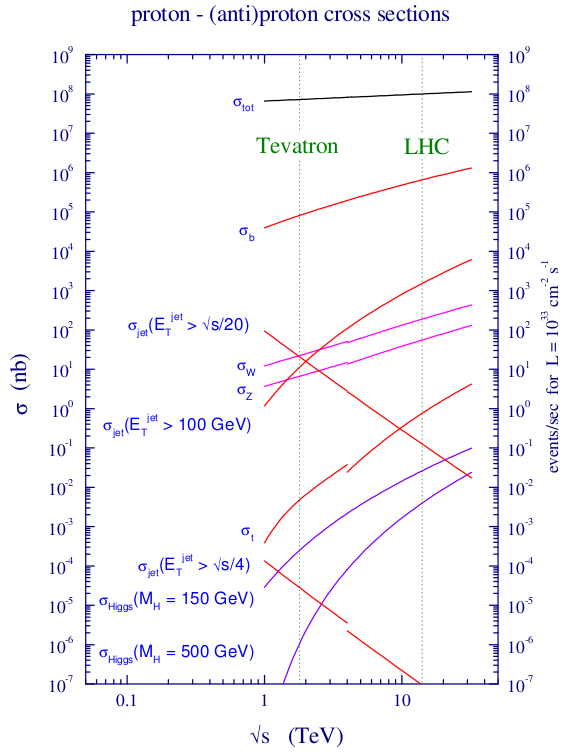
\includegraphics[width=0.85\textwidth]{xsec.png}
  \caption[The theoretical production cross sections as a function of centre of
mass energy for several Standard Model processes.] {The theoretical production
cross sections as a function of centre of mass energy for several Standard Model
processes such as the b quark production cross section, $\sigma_{b}$, and the
Higgs boson production cross sections, $\sigma_{Higgs}$.  $\sigma_{tot}$ is the
total inelastic cross section.  The cross sections that are of relevance to this
thesis analysis are the \PW and \PZ boson cross sections $\sigma_{\PW}$ and
$\sigma_{\PZ}$ respectively.  From \cite{campbell2006hard}.}

  \label{fig:LHCxsec}
\end{figure}

The LHC is part of a larger accelerator complex as shown in 
\FigureRef{fig:LHCcomplex}. Hydrogen gas is first ionised to produce a cloud of
protons, which are then accelerated by the LINAC2 linear accelerator to
\unit{50}{\MeV}.  Before being injected into the Proton Synchrotron (PS) the
protons are injected into the Proton Synchrotron Booster (PSB) and accelerated
to \unit{1.4}{\GeV}. In the PS the protons are grouped into bunches and the
energy is increased to \unit{25}{\GeV}. The bunches are then accelerated in the
Super Proton Synchrotron (SPS) to \unit{450}{\GeV} and then injected into the
LHC.

\begin{figure}[htbp]
  \centering
  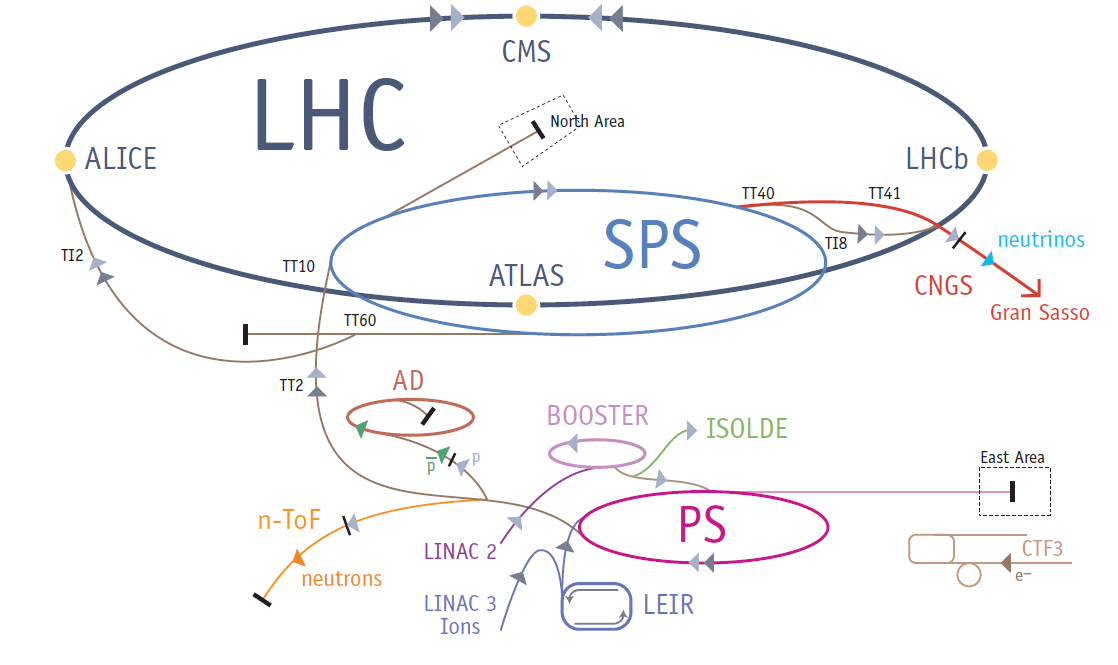
\includegraphics[width=0.96\textwidth]{accelerators.png}
  \caption{The LHC complex.}
  \label{fig:LHCcomplex}
\end{figure}

There are four main experiments studying the collisions at the
{LHC}.  
ALICE\footnote{A Large Ion Collider Experiment.} is designed to study the quark
gluon plasma that will be produced in the heavy ion collisions
\cite{aamodt2008alice}.
The LHCb\footnote{Large Hadron Collider beauty.} experiment is designed to study
B-meson decays to measure CP violation \cite{alves2008lhcb}.
ATLAS\footnote{A Toroidal LHC Apparatus.} and CMS\footnote{Compact Muon
Solenoid.} are general purpose detectors that are designed to search for a wide
range of new physics \cite{chatrchyan2008cms,aad2008atlas}.

In addition there are two smaller special-purpose detectors.
The LHCf \footnote{Large Hadron Collider forward.} is an experiment designed to
measure the neutral particles emitted in the very forward region of LHC
collisions.  The goal of the experiment is to provide data for hadron
interaction models that are used in the study of extremely high-energy
cosmic-rays \cite{adriani2008lhcf}.
The goal of the TOTEM\footnote{TOTal Elastic and diffractive cross section
Measurement.} experiment is to measure the total proton-proton
cross section and study the elastic and diffractive scattering at the LHC. The
detector is located at either side of the CMS detector \cite{anelli2008totem}.

\subsection{Operational History}
In September 2008 the {LHC} was commissioned and the first beams were
circulated.  Before the first collisions could be delivered an interconnection
between two of the dipole magnets failed. This led to
a large amount to helium rapidly evaporating which caused considerable damage to
the machine \cite{lebrun2009sector}.  Due to this incident it was decided that,
after the repairs,
the {LHC} should be run at a lower centre of mass energy of \unit{7}{\TeV} until
the quench protection system could be upgraded and the interconnections
thoroughly verified for higher currents \cite{myers2010lhc}.

The {LHC} was repaired by the end of 2009 and the first collisions at a record
energy of \unit{2.36}{\TeV} were delivered in November.  From March to November
2010 the {LHC} operated at \unit{7}{\TeV} delivering \unit{46.4}{\invpb} of
proton-proton collisions of which \unit{36.1}{\invpb} was certified for analysis
\cite{myers1990design}.  In November and December 2010 the {LHC} produced lead
ion collisions at \unit{2.36}{\TeV}.

\begin{figure}[htbp]
  \centering
  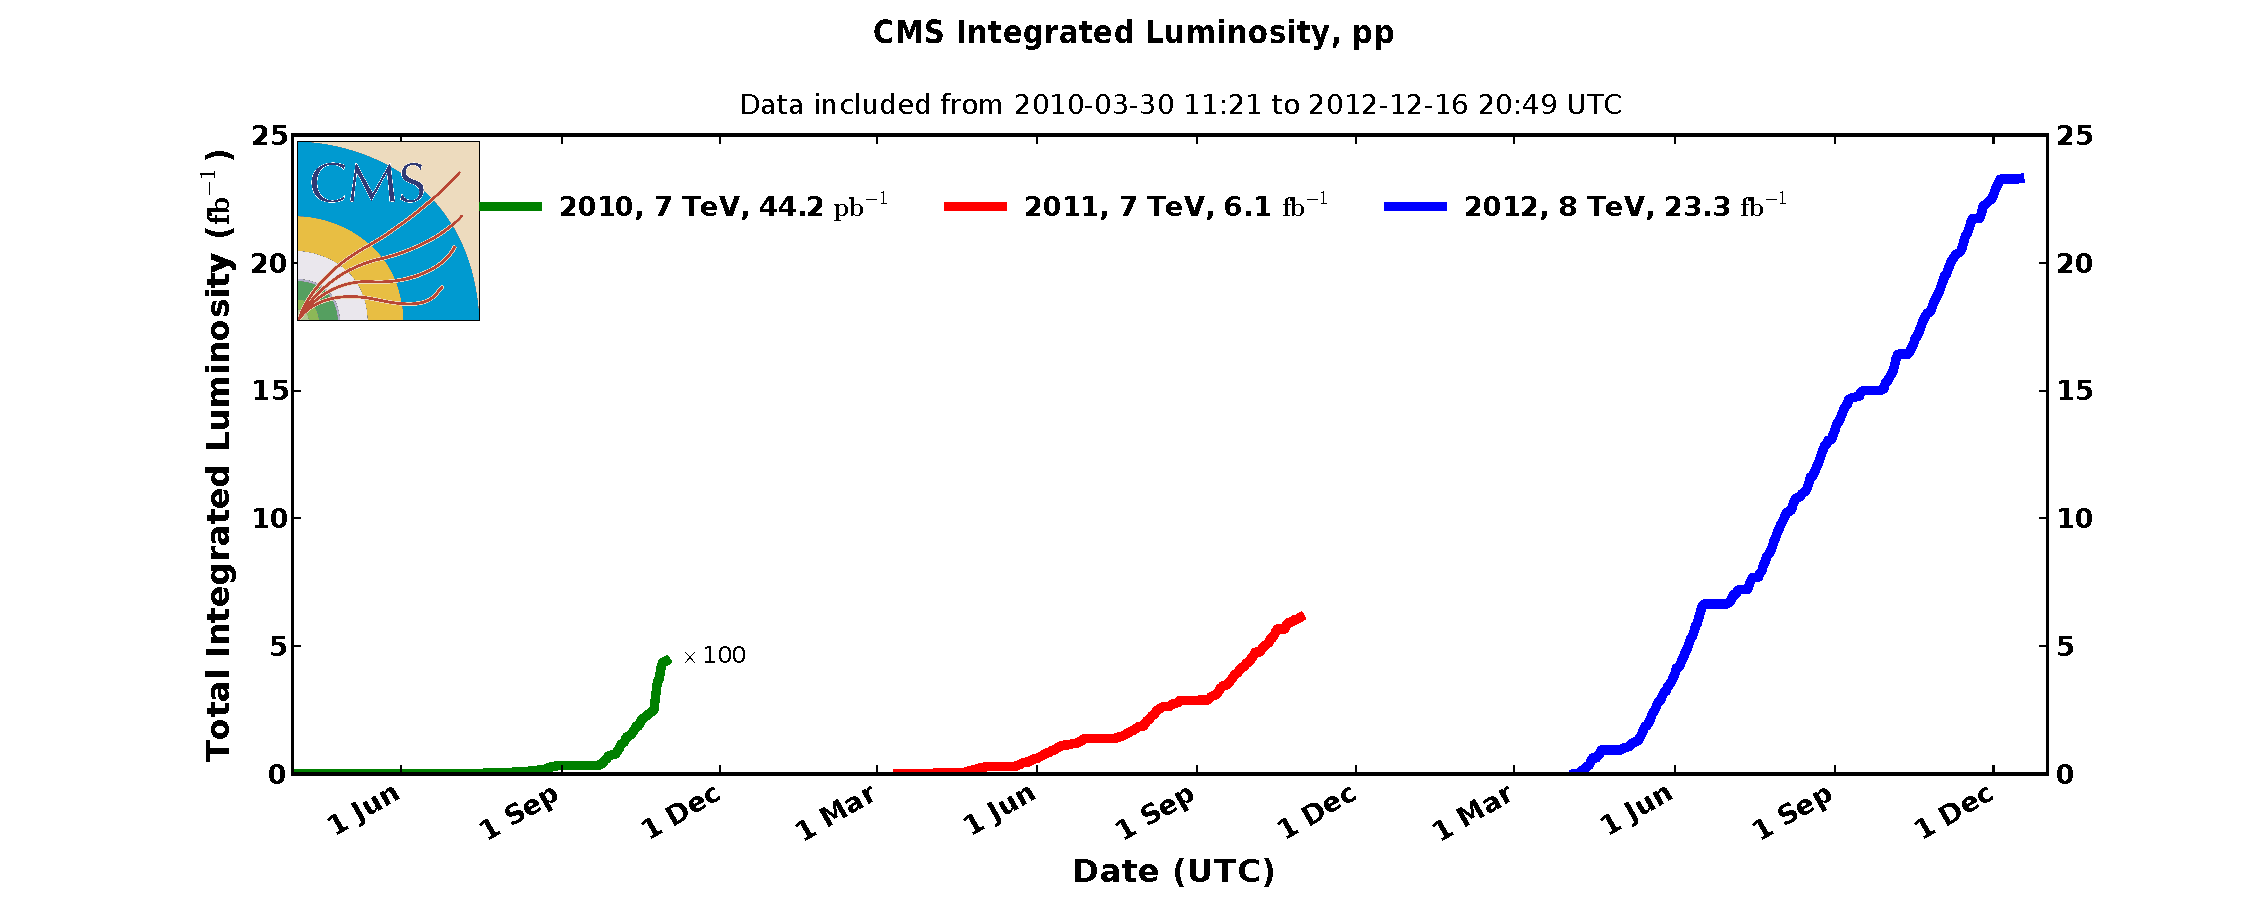
\includegraphics[width=\textwidth]{int_lumi_cumulative_pp_1}
  \caption[The luminosity delivered by LHC and recorded by CMS in 2010, 2011 and
2012.] {The luminosity delivered by LHC and recorded by CMS in 2010, 2011 and
2012. From \cite{intlumi}.}
  \label{fig:LHC2010}
\end{figure}

The target for running in 2011 was to deliver \unit{1}{\invfb} of data. This was
achieved by June. The target was increased to \unit{5}{\invfb} of data for 2011 which was achieved by October. 
In 2012 the {LHC} was operated at a centre of mass energy of \unit{8}{\TeV}
and a total of \unit{22.1}{\invfb} of data was collected by December.
The luminosity delivered by LHC and recorded in CMS in 2010, 2011 and 2012 is
shown in \FigureRef{fig:LHC2010} \cite{intlumi}.

The analysis presented in the following chapters is based on the
\unit{36.1}{\invpb} of data from  2010 and \unit{840}{\invpb} of data from the first half of 2011.

\section{CMS Detector}
{CMS}\cite{chatrchyan2008cms} is one of the two general purpose
detectors designed to study LHC collisions. The main design parameters for the
{CMS} detectors  are listed in \TableRef{tab:cmsparam}.

\begin{table}[htbp]
\begin{center}
\begin{tabular}{ l l }
\toprule
Parameter & CMS \\
\midrule
Total weight (tons)                 & $12,500$  \\
Overall diameter (m)                & $15$  \\
Overall length (m)                  & $20$  \\
Magnetic field for tracking (T)     & $4$  \\
Solid angle for energy measurements ($\Delta\phi \times \Delta\eta$)   
                                    & $2\pi \times 9.6$  \\
Solid angle for precision measurements ($\Delta\phi \times \Delta\eta$)   
                                    & $2\pi \times 5.0$  \\
Total cost (CHF)                    & $550\times 10 ^{6}$  \\
\bottomrule
\end{tabular}
\caption[Main design parameters of the CMS detector.]{Main design parameters of
the CMS detector. From \cite{froidevaux2006general}.\label{tab:cmsparam}}
\end{center}
\end{table}

The design goals of the CMS detector are:
\begin{itemize}
  \item Good muon identification and momentum resolution and the ability to
unambiguously assign charge to muons with $\PT < \unit{1}{\TeV}$
  \item Good charged particle momentum resolution and reconstruction in the
tracker.
  \item Good electromagnetic energy resolution. 
  \item Good resolution of missing transverse energy and dijet mass.
\end{itemize}

The design of CMS meets these requirements while overcoming significant
experimental challenges.  At design luminosity, approximately 1 billion
inelastic events will occur in CMS every second, whereas CMS is limited to
storing the data of only $\approx 100 $ events within that time.  The detector
must be able to reduce this rate with a trigger to accept events that are
interesting from a physics perspective and reject events otherwise.

In addition to this challenge, each event of interest will have on average 20
inelastic events superimposed on it. This results in around 1000 charged
particles produced every \unit{25}{\ns}, which require the detectors to
have a high granularity with a good time resolution to ensure a low occupancy.
The large flux of particles will also produce high radiation levels which 
required radiation hard detectors and electronics.

\begin{figure}[htbp]
  \centering
  \includegraphics[width=0.98\textwidth]{cms_120918_02}
  \caption[Diagram of the CMS detector.] {Diagram of the CMS detector. From
\cite{SketchUpCMSGallery}.}
  \label{fig:CMSnc}
\end{figure}

An overview of the detector is shown in \FigureRef{fig:CMSnc}.  Starting at the
interaction point in the centre of the detector and moving radially outwards,
CMS comprises the pixel tracker, the silicon microstrip tracker, the
lead-tungstate electromagnetic calorimeter, the sampling brass-plate hadronic
calorimeter, a \unit{4}{\tesla} superconducting solenoid magnet, an outer
hadronic calorimeter and four muon chambers.


\subsection{Magnet}
A large superconducting solenoid provides the basis for the design of the CMS
detector, and is the main structural support for the detector components in the
barrel region.

The superconducting magnet in CMS produces a \unit{4}{\tesla} field in a bore of
\unit{6}{\meter} diameter and \unit{12.5}{\meter} length.  While operating at
full current the magnet stores \unit{2.6}{\giga\joule} of energy.  A large
magnetic field is needed to give CMS a large bending power and the ability to
precisely measure the momentum of high-energy charged particles.  The solenoid
bore is large enough that the tracking detectors and the calorimetry can fit
inside it\cite{chatrchyan2008cms}.

The magnetic flux is returned through a \unit{1.8}{\meter} thick saturated iron
yoke which is interleaved with the muon detector.

\subsection{Tracking}
The inner tracker is designed to accurately and efficiently measure the
trajectories of charged particles produced in collisions at the centre of CMS.
The tracker is also required to be able to reconstruct secondary vertices from
the decay of long-lived particles.  At the design luminosity of the LHC it
is expected that every \unit{25}{\ns} an average of 1000 particles will traverse
the inner detector; therefore, it is required that the tracker has a high
granularity and a fast response while remaining resilient to radiation damage. 

\begin{figure}[htbp]
  \centering
  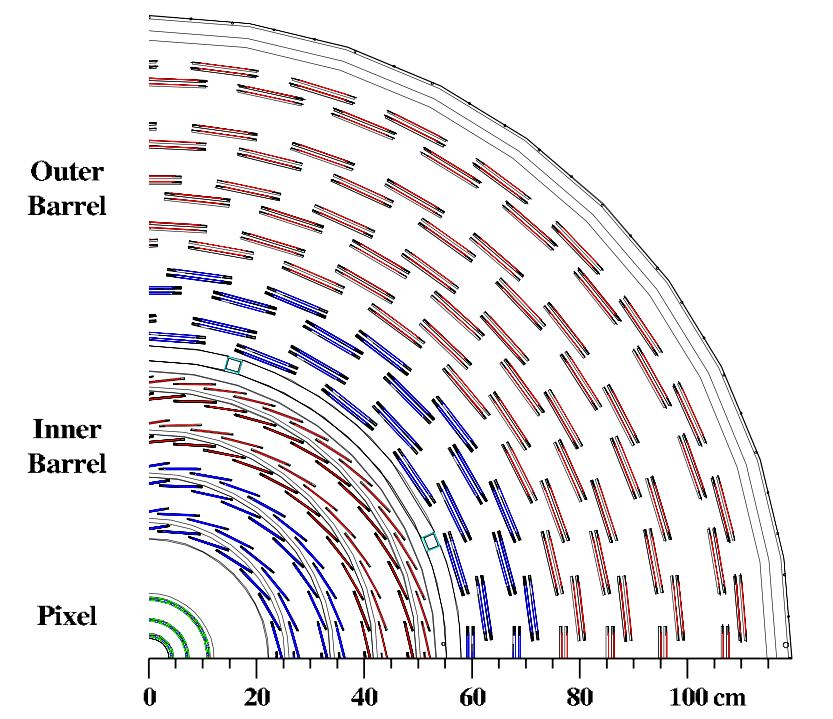
\includegraphics[width=0.6\textwidth]{tracker}
  \caption[A quadrant of the cross section of the barrel part of the {CMS}
tracker.]{A quadrant of the cross section of the barrel part of the {CMS}
tracker. From \cite{cmsgsf}.}
  \label{fig:tracker}
\end{figure}

A quadrant of the cross sections of the barrel part of the {CMS}
tracker is shown in \FigureRef{fig:tracker}.
The tracker utilises silicon pixel detectors in the innermost layers where the
particle flux is the highest.  Outside of the pixel detector, the tracking
detector comprises several layers of silicon microstrip detectors where the
particle flux is smaller.  The total active area of silicon in the CMS tracker
is over \unit{200}{\meter\squared} \cite{chatrchyan2008cms}.

\subsubsection{Pixel Tracker}
The pixel tracker consists of three layers of hybrid silicon pixel detectors in
the barrel region and two in the endcap region. 
The barrel layers are positioned at radii of 4.4, 7.3 and \unit{10.2}{\cm} and have
a length of \unit{53}{\cm}. The two layers in each endcap are located at
$|z|=34.5$ and \unit{46.5}{\cm} with an inner radius of \unit{6}{\cm} and an
outer radius of \unit{15}{\cm}.

\begin{figure}[htbp]
  \centering
  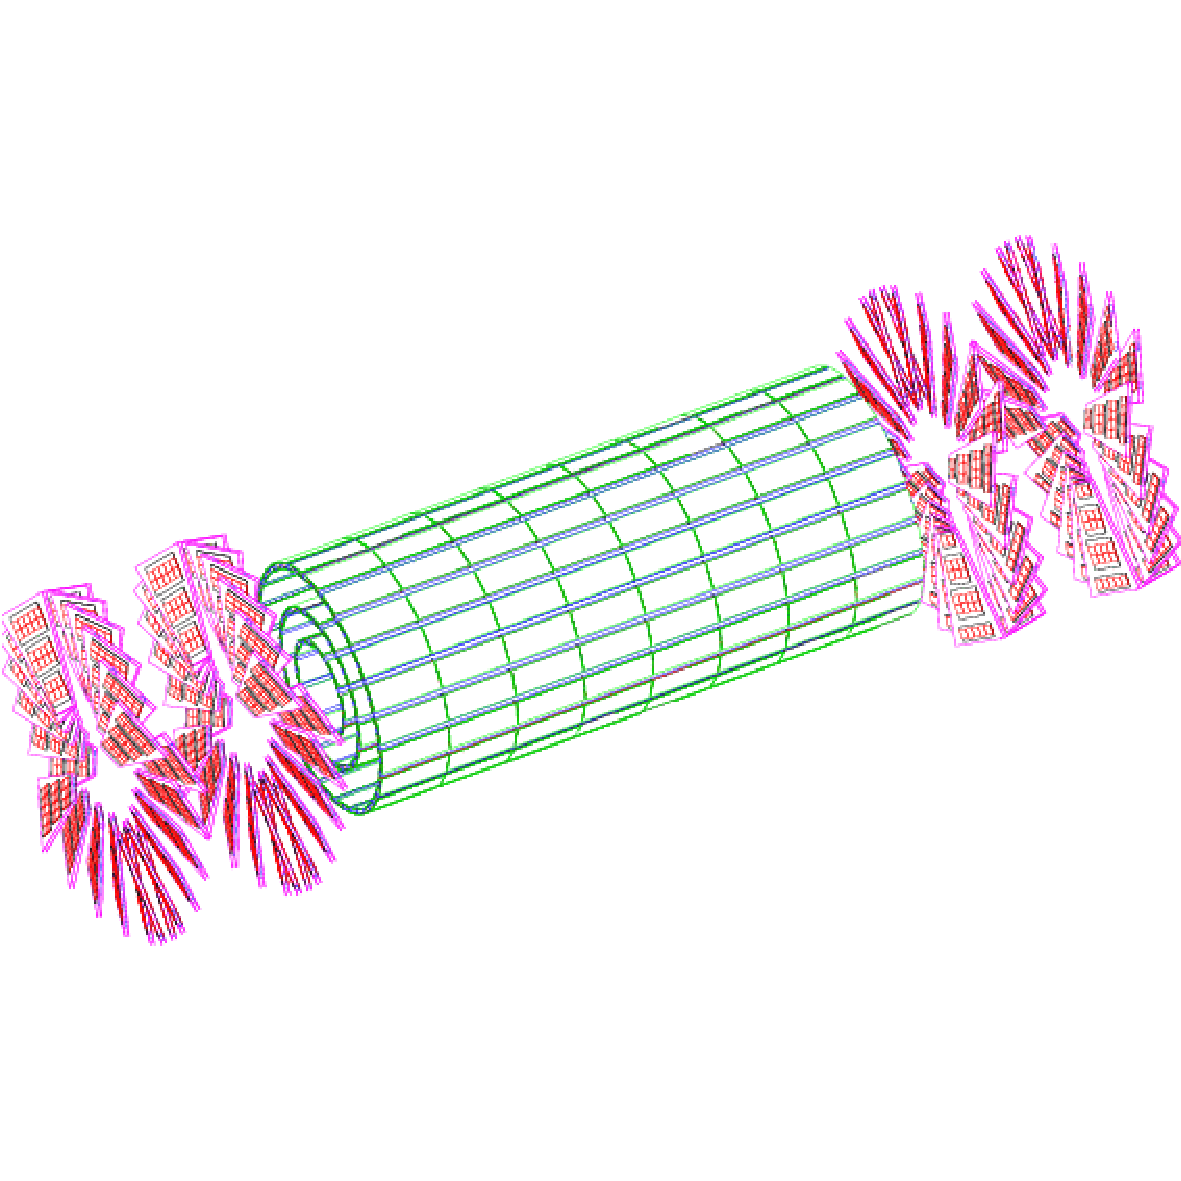
\includegraphics[width=0.75\textwidth]{pixel}
  \caption[The layout of pixel detector in the CMS tracker.]
  {The layout of pixel detector in the CMS tracker. From \cite{chatrchyan2008cms}.}
  \label{fig:pixel}
\end{figure}

A close up view of the pixel tracker is shown in \FigureRef{fig:pixel}.  
Each pixel has a surface area of \unit{$100\times150$}{\micron} which results in
an average particle occupancy of $\mathcal{O}(10^{-4})$ per pixel per crossing.

\subsubsection{Strip Tracker}
The barrel strip tracker comprises two parts, the inner (TIB) and outer (TOB)
trackers.  The TIB is made of 4 layers and covers the longitudinal region $|z|
< \unit{65}{\cm}$ and the region \unit{$20<r<55$}{\cm} in the radial direction.
The TIB utilises microstrip detectors with a cell size of
$\unit{10}{\cm}\times\unit{80}{\micron}$ with an average occupancy of
$\approx\unit{2-3}{\%}$.

The TOB is formed of 6 layers with a half-length of $|z| < \unit{110}{\cm}$. In
this region the flux is low enough to allow for the use of larger pitch
silicon microstrips with a cell size of
$\unit{25}{\cm}\times\unit{180}{\micron}$ with an average occupancy of
$\approx\unit{1}{\%}$.

The endcaps are separated into the Tracker End Cap (TEC) and the Tracker Inner
Disks (TID). The TEC is split into nine disks and covers the region
$\unit{120}{\cm} < |z| < \unit{280}{\cm}$. The TID comprises three rings
and fills the gap between the TEC and the TIB.

%\subsubsection{Performance}

\subsection{Electromagnetic Calorimeter}
The electromagnetic calorimeter (ECAL) is designed to measure the energy of
electrons and photons with a high resolution. It has a fine lateral granularity
to help with shower separation. It is a hermetic, homogeneous calorimeter
comprising 61200 individual lead tungstate ($PbWO_{4}$) scintillation crystals
in the barrel region ($|\eta|<1.479$) closed by 7324 crystals in each of the two
endcap parts ($1.479<|\eta|<3.0$) \cite{ecal1997technical}.

Lead tungstate crystals are ideally suited for this since the scintillation
decay time is similar to the LHC bunch crossing time, 
with $80\%$ of light being produced within \unit{25}{\ns}.
They also have a short radiation length ($X_0=\unit{0.89}{\cm}$) 
and Moliere radius (\unit{2.2}{\cm}) as well as being radiation hard
(up to \unit{10}{\mrad}).

A disadvantage to using lead tungstate is that the light output of the crystals
is relatively low and changes with temperature. This is overcome by using
photodetectors with an intrinsic gain and maintaining a stable temperature
(within \unit{0.1}{\degreecelsius}).

Silicon avalanche photodiodes (APDs) are used to detect the scintillation light
in the barrel and vacuum phototriodes (VPTs) are used in the endcap parts.

The barrel section of the ECAL (EB) surrounds the inner tracker. It comprises 36
identical supermodules that each cover a half length of the barrel
($0<|\eta|<1.479$) and \unit{20}{\degree} in $\phi$. Each supermodule contains 1700
crystals arranged in a $\phi$-$\eta$ grid with each crystal mounted in a
``semi-projective'' geometry, and aligned \unit{3}{\degree} off the nominal
interaction vertex.  The alignments in the longitudinal and transverse planes
are shown in \FigureRef{fig:crystaltilt} and \FigureRef{fig:crystallong}
respectively. The non-pointing geometry prevents particles escaping through the
gaps between the crystals \cite{ecal1997technical}.  Each crystal has a
cross section of \unit{$22 \times 22$}{\mm\squared} and a length of
\unit{230}{\mm} ($\unit{25.8}{X_0}$).

\begin{figure}[p]
  \centering
  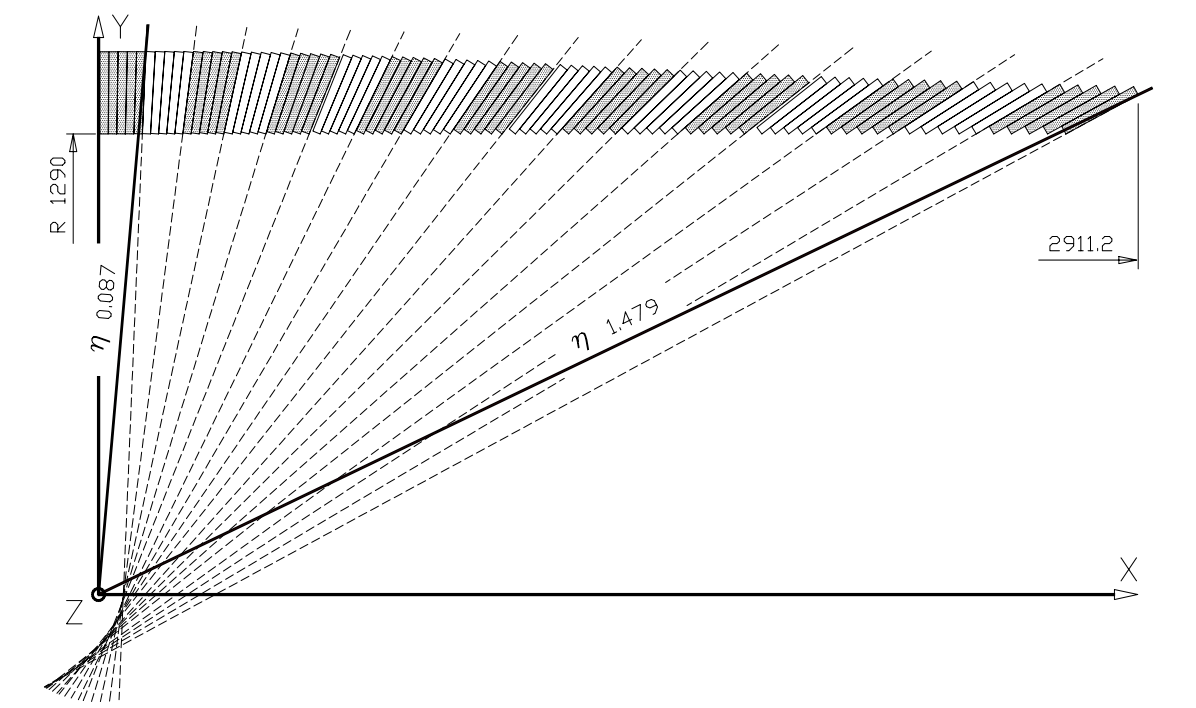
\includegraphics[width=0.7\textwidth]{crystallong}
  \caption[The crystal alignment in the longitudinal view.]{The crystal
alignment in the longitudinal view. The dotted lines show the alignment of the
edge of the crystals. A single supermodule is shown. From \cite{ecal1997technical}.}
  \label{fig:crystallong}
\end{figure}

\begin{figure}[p]
  \centering
  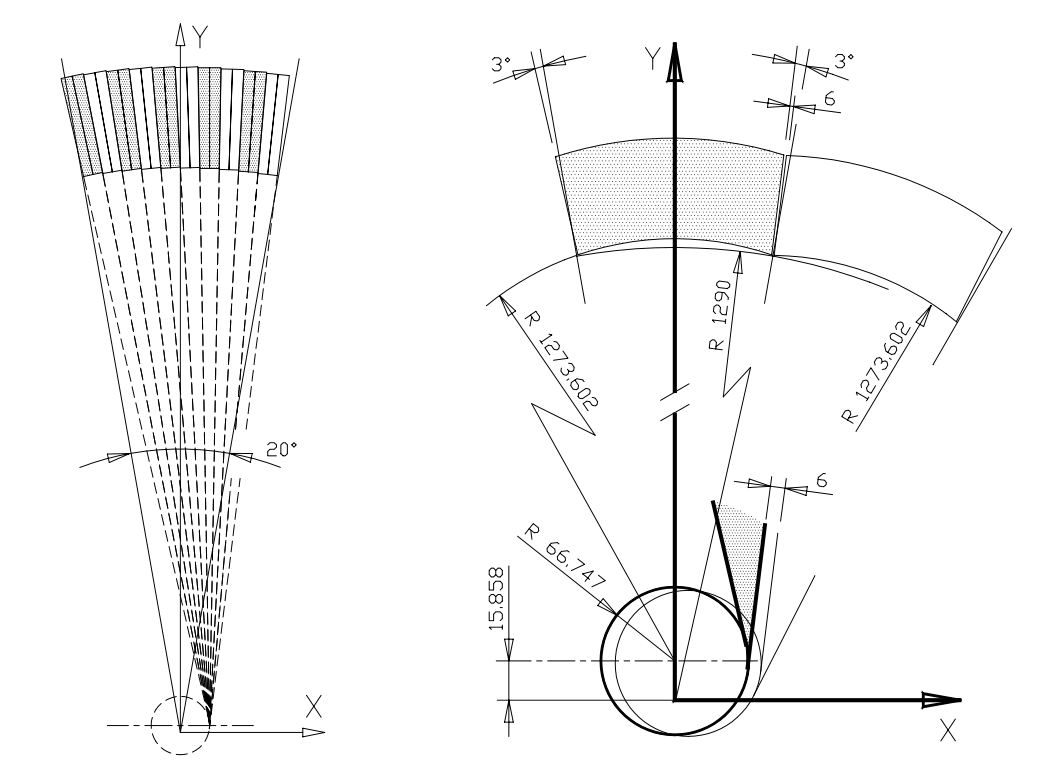
\includegraphics[width=0.7\textwidth]{crystaltilt}
  \caption[The tilt of the ECAL crystals in the transverse plane and the
alignment of the supermodules.] {The tilt of the ECAL crystals in the transverse
plane (left) and the alignment of the supermodules (right). The dotted lines
show the alignment of the crystal edges. From \cite{ecal1997technical}.}
  \label{fig:crystaltilt}
\end{figure}

The endcaps (EE) are formed of two ``Dees'', semi-circular aluminium plates
which support the ``supercrystals'', $5\times5$ arrays of crystals. The crystals are
mounted to point away from the nominal interaction vertex by a small angle in a similar way
to the barrel. 
Unlike the barrel the crystals are arranged in an $x$-$y$ grid.
Installed in front of the endcap ECAL is a preshower system which helps with
the rejection of \Ppizero \cite{chatrchyan2008cms}.

\subsubsection{Performance}

Using a \unit{100}{\GeV} test beam, the energy resolution of the {ECAL} was
found to be\cite{chatrchyan2008cms},
\begin{align}
\left(\frac{\sigma}{E}\right)^{2} 
&= \left(\frac{S}{\sqrt{E}}\right)^{2} + \left(\frac{N}{E}\right)^{2} + C^{2}\\
&=
\left(\frac{\unit{2}{\%}}{\sqrt{E}}\right)^{2} +
\left(\frac{\unit{124}{\MeV}}{E}\right)^{2} + 
\left(\unit{0.26}{\%}\right)^{2}  
\end{align}
where $S$ is the stochastic term, $N$ is the noise term and $C$ is the constant
term. The measured {ECAL} energy resolution is shown in \FigureRef{fig:ECAL}. The
stochastic term is due to the statistical fluctuations in the particles produced
in the electromagnetic shower. The noise term is due to electronic noise and
pile-up. The constant term is due to errors such as non-uniform signal
generation and calibration errors \cite{chatrchyan2008cms}.

\begin{figure}[htbp]
  \centering
  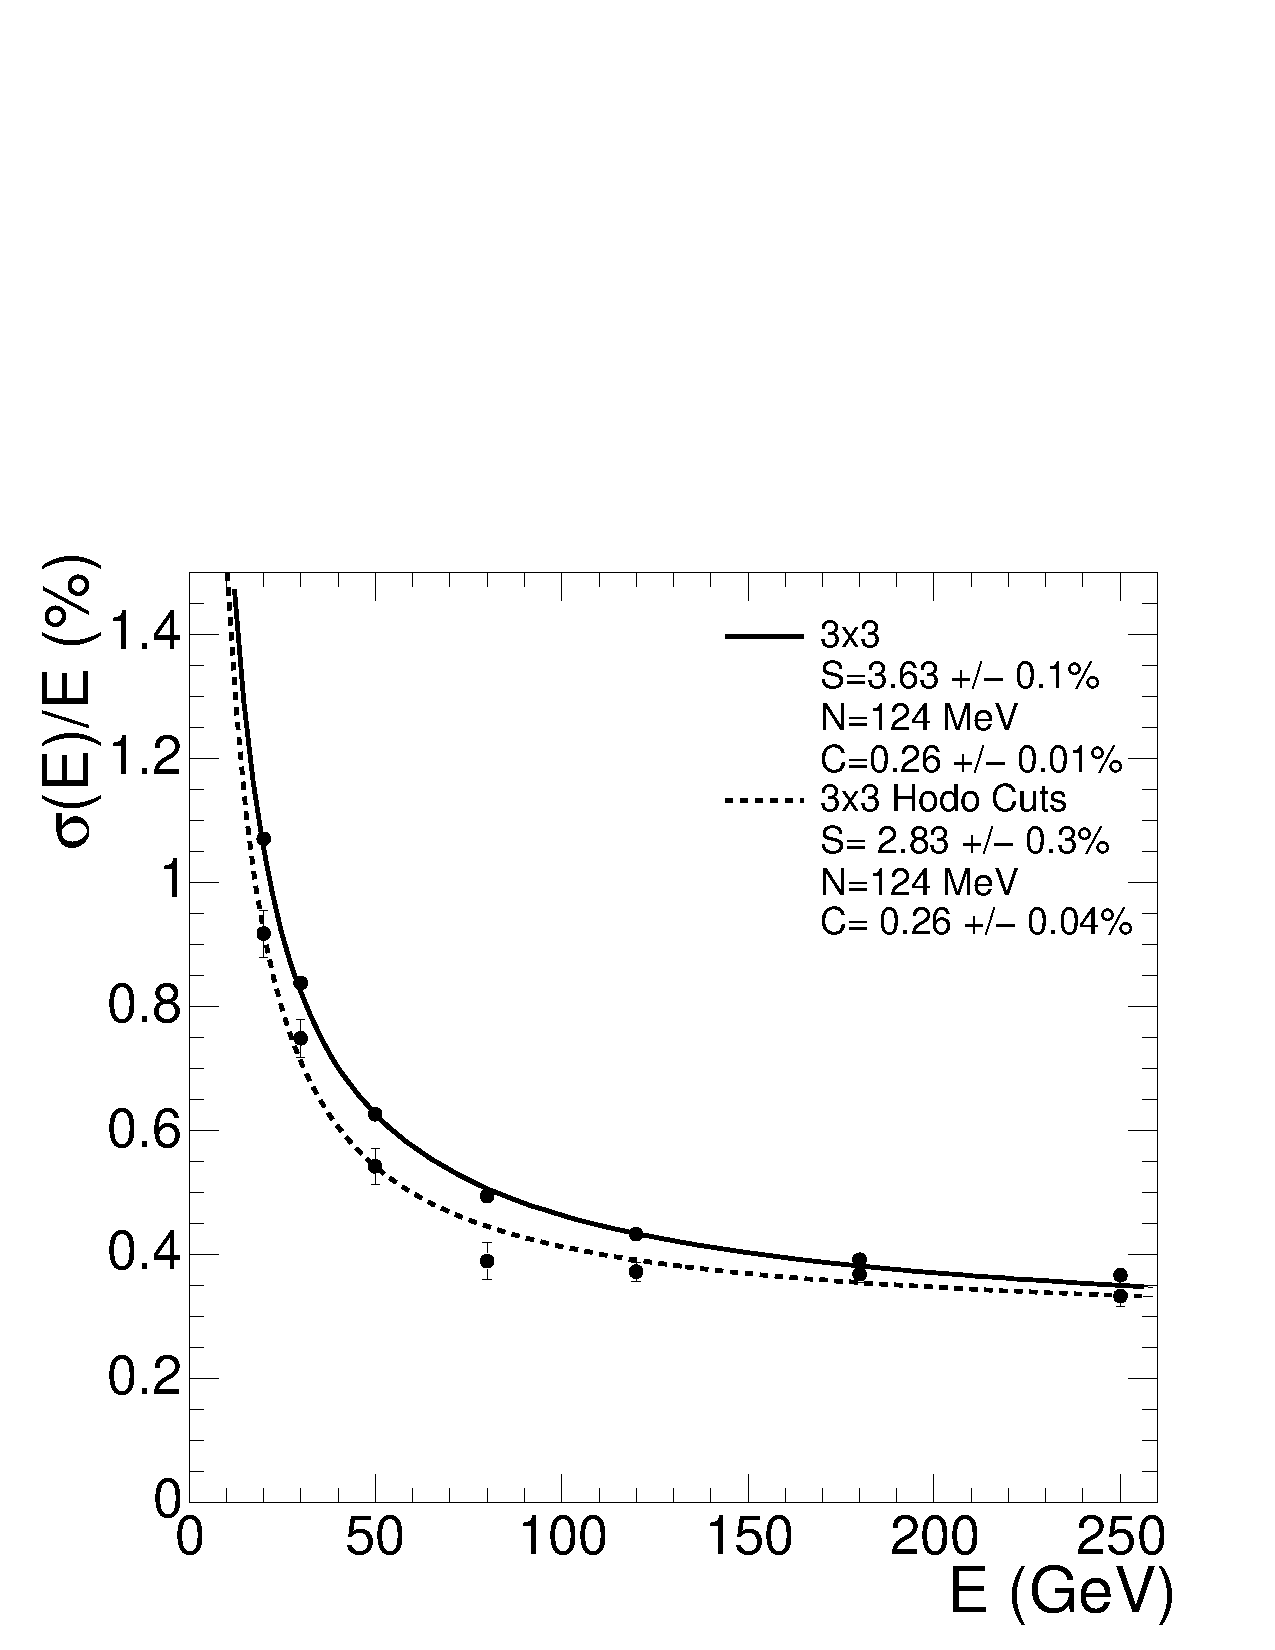
\includegraphics[width=0.7\textwidth]{ecal_performance}
  \caption[Energy resolution $\nicefrac{\sigma}{E}$ of ECAL as a function of
electron energy $E$]{Energy resolution $\nicefrac{\sigma}{E}$ of ECAL as a
function of \label{fig:ECAL} electron energy $E$. From
\cite{chatrchyan2008cms}.}
\end{figure}

\subsection{Hadronic Calorimeter}
The hadronic calorimeter (HCAL), in addition to the electromagnetic calorimeter,
is designed to measure the energy of hadron jets and the missing transverse
energy (\met) which are important signatures in many physics studies at the LHC.

The {HCAL} is a brass/scintillator
sampling hadron calorimeter that covers the region up to $|\eta|<3.0$.  The
scintillation light is channelled by wavelength shifting fibres, that are
embedded in the scintillation tiles, to hybrid photodiodes that can operate in
the high axial magnetic field \cite{chatrchyan2008cms}.

The barrel hadron calorimeter (HB) covers the region ($|\eta| < 1.4$)
and the hadron endcap covers the region $1.4 < |\eta| < 3.0$.

The barrel hadron calorimeter is positioned between the ECAL and the inside of
the solenoid magnet coil ($\unit{1.77}{\meter}<r<\unit{2.95}{\meter}$).  The
strong constraints imposed by the dimensions of the solenoid magnet results in
the HB having an insufficient amount of material to absorb the hadronic shower
in the central region.  To overcome this limitation the outer hadronic
calorimeter (HO) or tail catcher, has been added around the solenoid magnet to
increase the effective thickness of the hadron calorimetry to over 10
interaction lengths.  This provides better protection against punch-through to
the muon system.

\subsubsection{The Forward Calorimeter}
In the forward region ($|\eta| > 3$) energy measurements are made with the
forward hadronic calorimeter, situated \unit{11}{\meter} from the interaction
point. The main role of the forward calorimeter is to improve the \ETm
measurement and to tag jets in the forward direction.

The forward hadronic calorimeter is an iron/quartz-fibre calorimeter where the
Cherenkov light is detected by photomultipliers.  The calorimeter needs to be
radiation hard due to the very large flux in the forward region. However, it is
still expected that after 10 years of operation the light output will be reduced by
about $30\%$ due to the level of radiation \cite{chatrchyan2008cms}. 

\subsubsection{Performance}

\FigureRef{fig:hcalperform} shows the jet energy resolution for three parts of
the {HCAL} measured in test beams. The granularity of the sampling in each
region of the HCAL is such that the resolution is similar in each.

\begin{figure}[htbp]
  \centering
  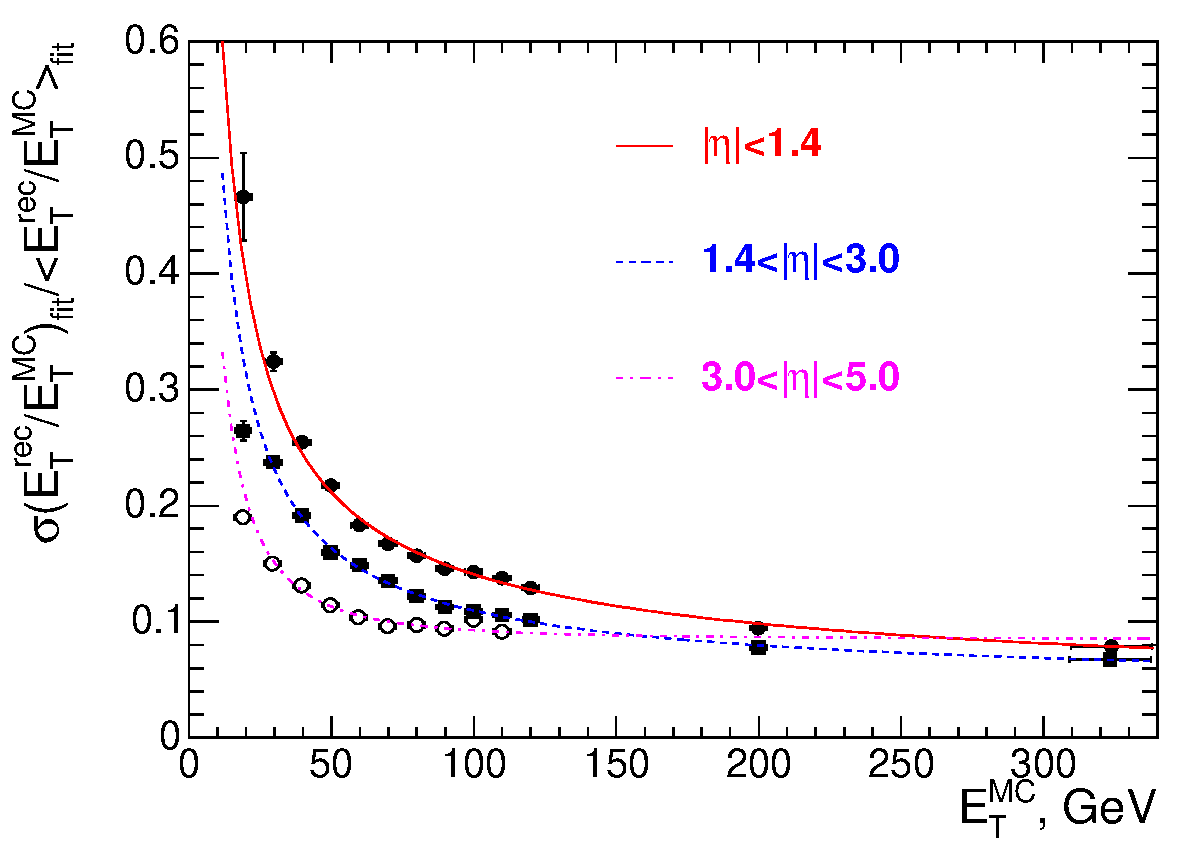
\includegraphics[width=0.7\textwidth]{hcal_performance}
  \caption[The jet transverse energy resolution as a function of jet transverse
energy.] {The jet transverse energy resolution as a function of jet transverse
energy for barrel jets ($|\eta| < 1.4$), endcap jets ($1.4<|\eta| < 3$) and
forward jets ($3<|\eta| < 5$). From \cite{chatrchyan2008cms}. }
  \label{fig:hcalperform}
\end{figure}

\begin{figure}[htbp]
  \centering
  \begin{subfigure}{0.48\textwidth}
    \centering
    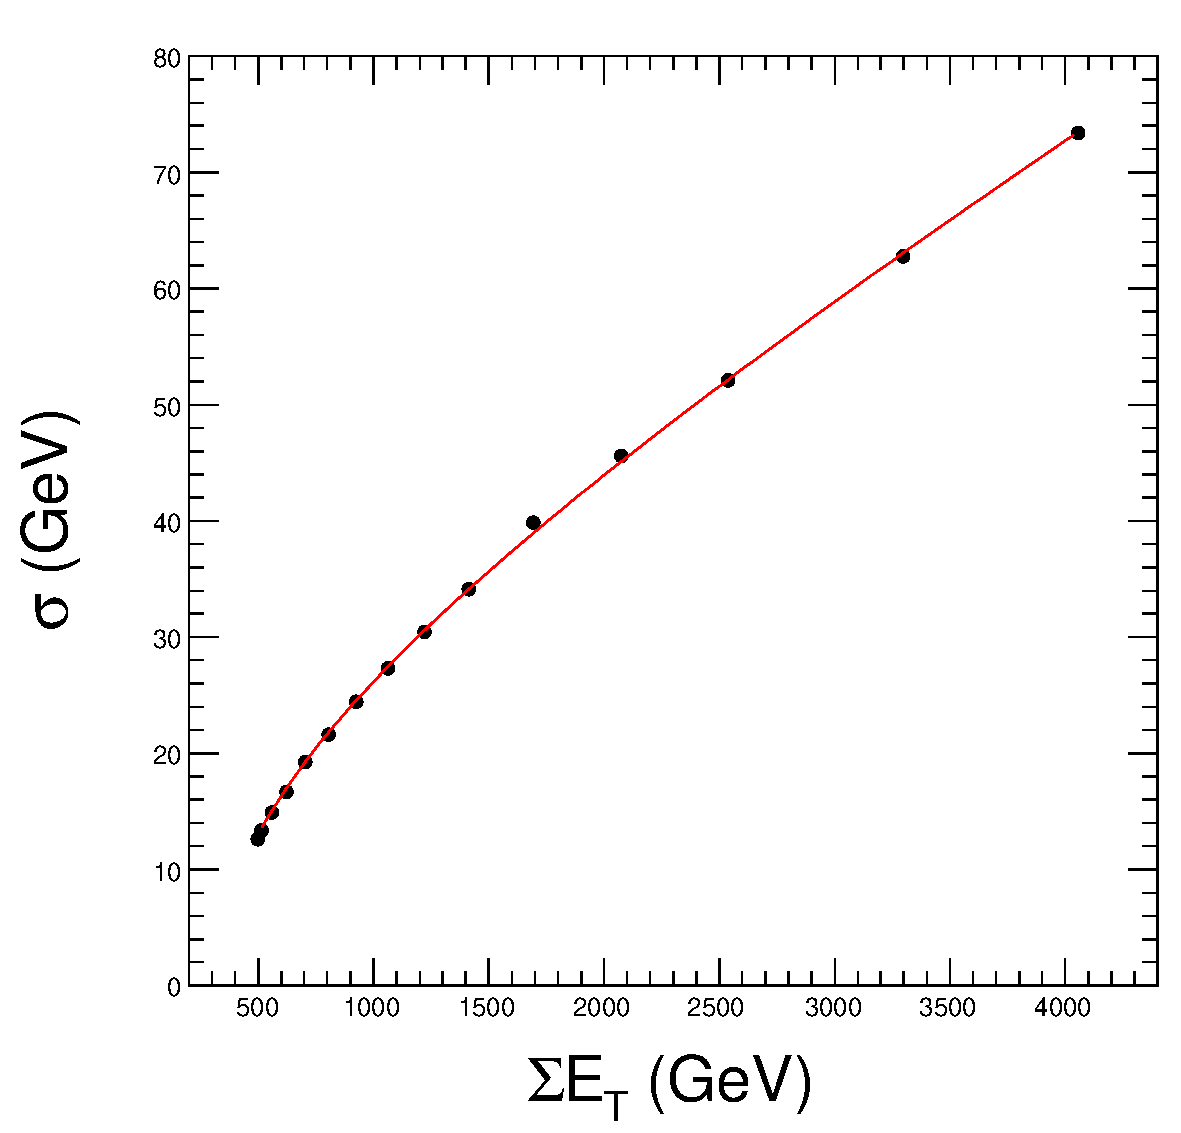
\includegraphics[width=\textwidth]{met_res}
    \caption{\ETm resolution.}
    \label{fig:met_res}
  \end{subfigure}
  \begin{subfigure}{0.48\textwidth}
    \centering
    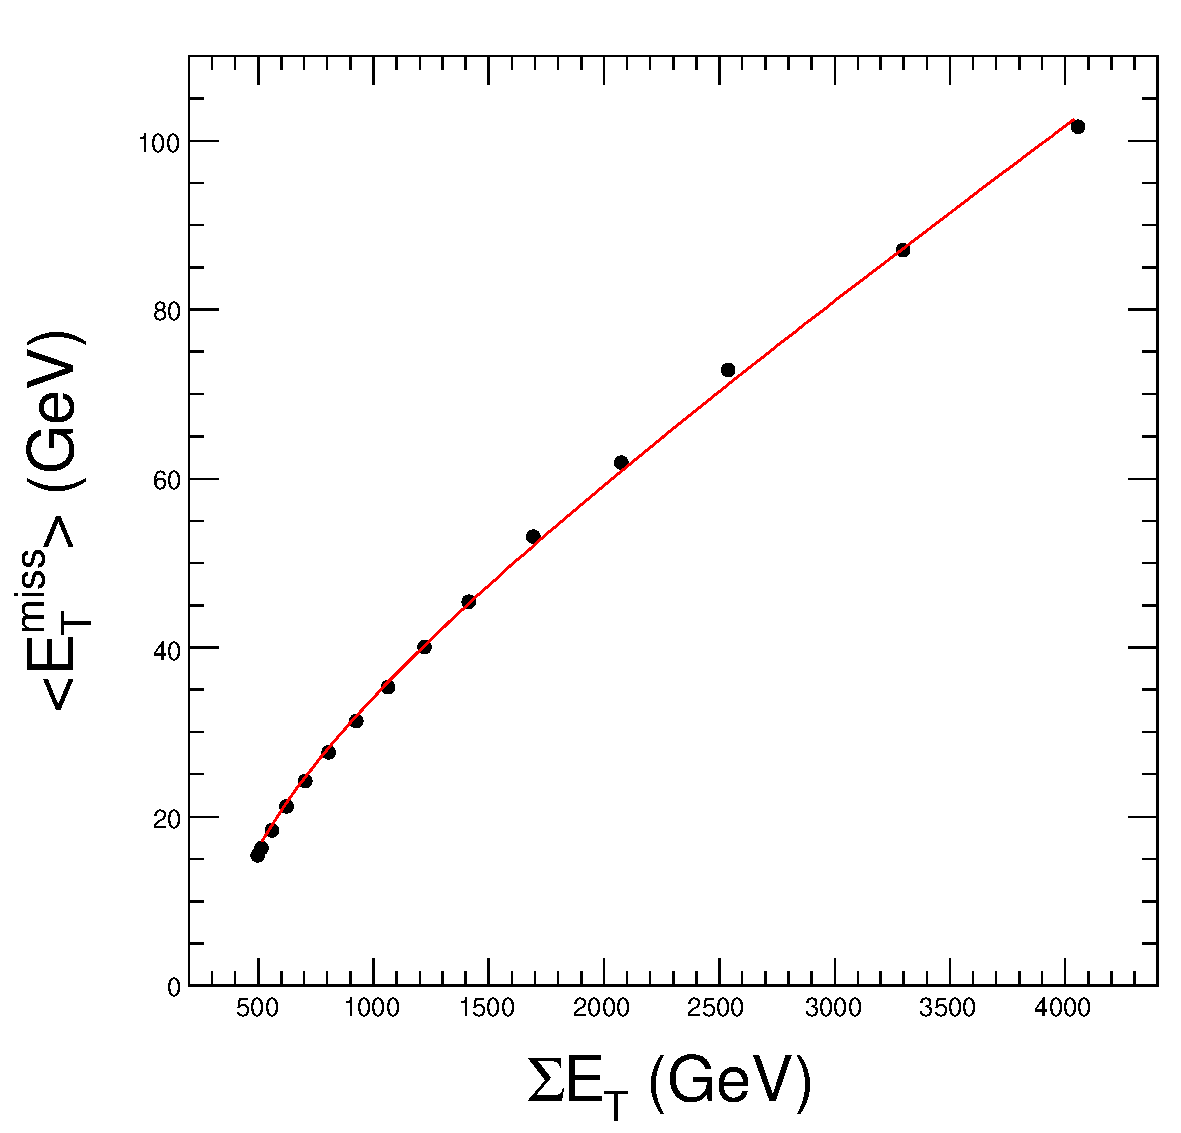
\includegraphics[width=\textwidth]{met_mean}
    \caption{Average reconstructed \ETm.}
    \label{fig:met_mean}
  \end{subfigure}
  \caption[The missing transverse energy performance as a function of the $\sum
E_T$ for QCD events.] { The missing transverse energy performance as a function
of the $\sum E_T$ for QCD events with pile-up. From \cite{chatrchyan2008cms}. }
  \label{fig:met_performance} 
\end{figure}

The performance of the missing transverse energy (\ETm) is shown in
\FigureRef{fig:met_performance} in QCD events. The \ETm resolution is
$\sigma(\ETm) \approx 1.0 \sqrt{\ET}\GeV$ and the average \ETm is
$\langle \ETm \rangle \approx 1.25 \sqrt{\ET}\GeV$
\cite{chatrchyan2008cms}.

\subsection{Muon System}
The muon system lies outside of the CMS solenoid and the outer HCAL detectors.
It is designed to have three functions; to identify muons, measure the momentum
of muons and trigger on muons. To perform these functions the muon system
consists of several different types of detectors due to the different background
rates and magnetic fields in each region of the detector.
The layout of the {CMS} muon system is shown in \FigureRef{fig:muon_system}.

\begin{figure}[htbp]
  \centering
  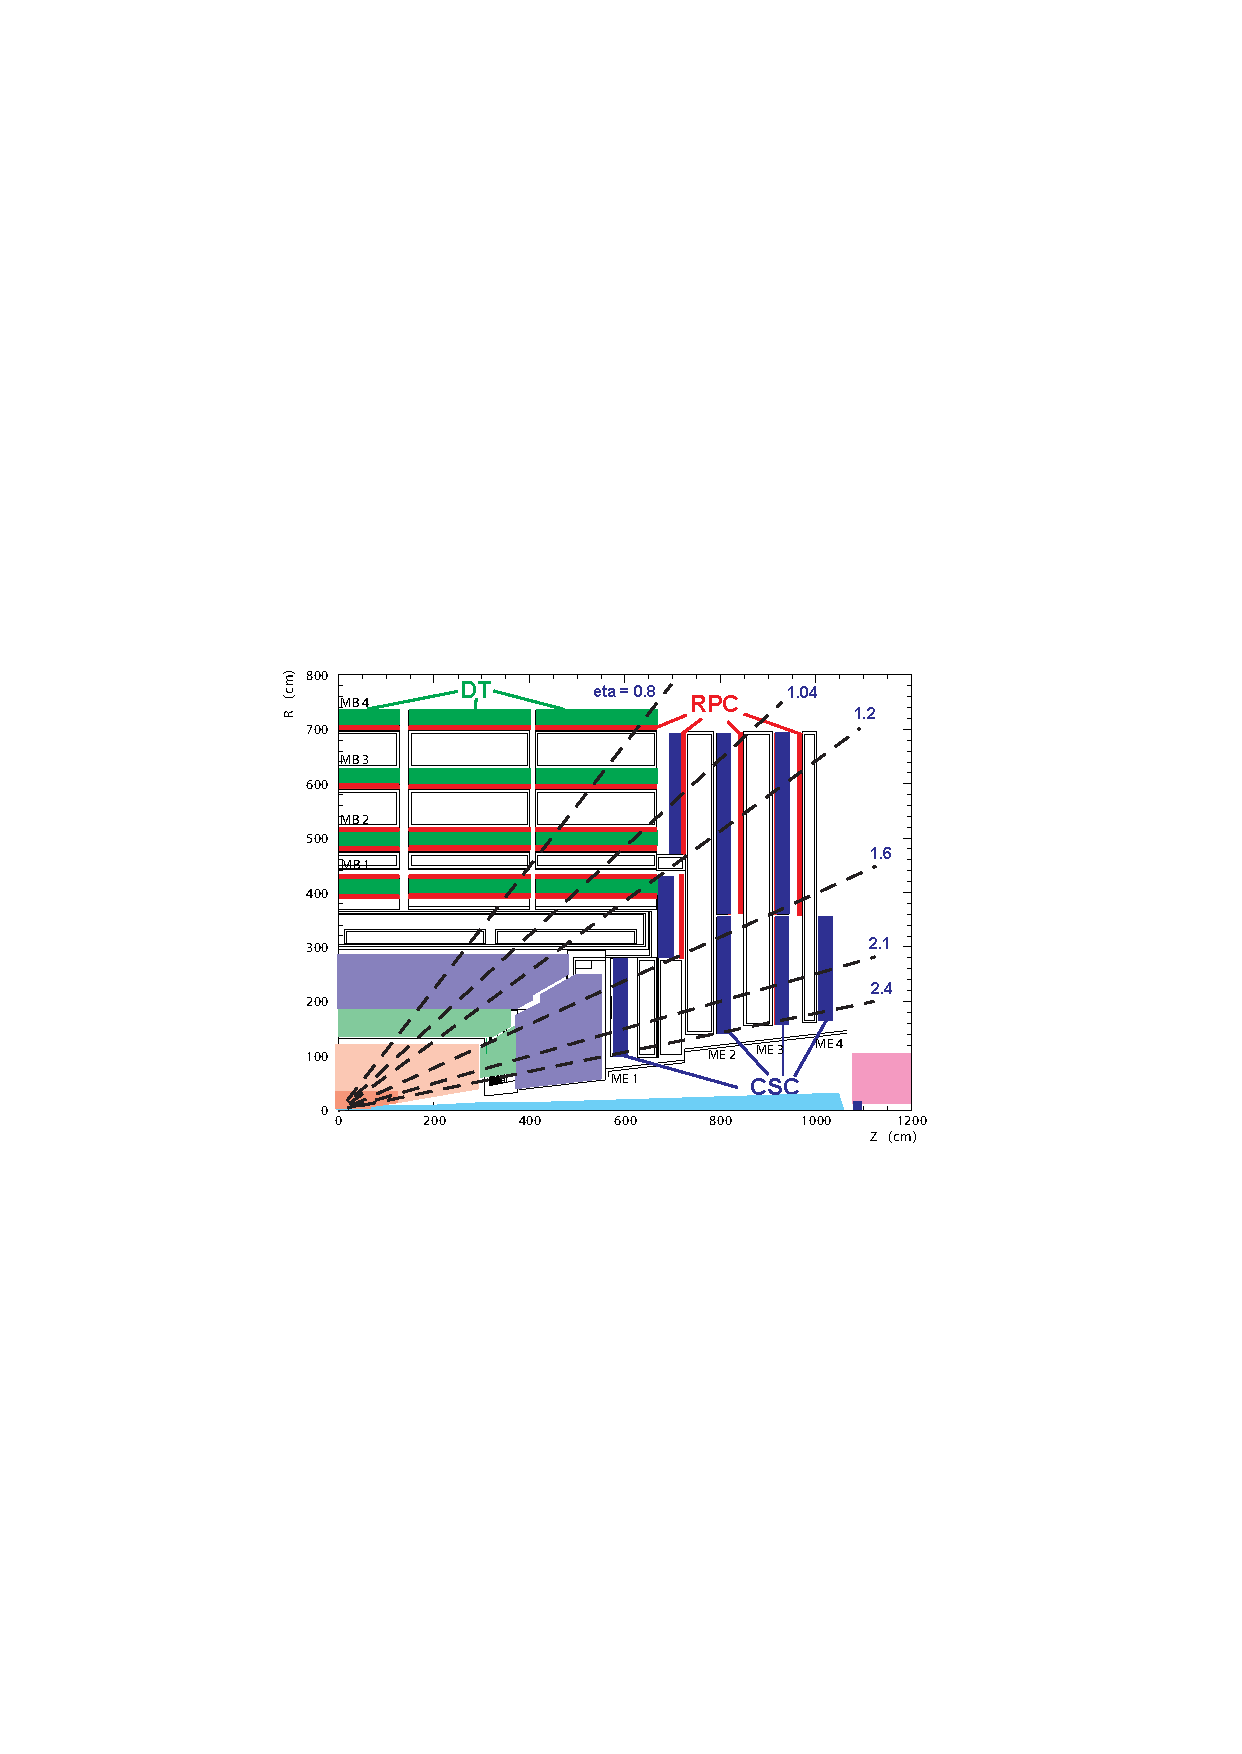
\includegraphics[width=0.8\textwidth]{muon_system}
  \caption[The layout of a quarter of the CMS muon system.] {The layout of a
quarter of the CMS muon system. From \cite{chatrchyan2008cms}.}
  \label{fig:muon_system}
\end{figure}

\subsubsection{Drift Tubes}
In the barrel region ($|\eta| < 1.2$)
where the background rate is low and the residual magnetic field is small,
 aluminium drift tubes (DT) are used,
arranged in four stations interleaved in the flux return
plates. 
Each station contains 12 layers, eight to measure the coordinate in the
$r$-$\phi$ plane and four to measure the $z$ direction (except the fourth station
which only measures the $r$-$\phi$ plane). 

\subsubsection{Cathode Strip Chambers}
In the endcaps ($0.9<|\eta|<2.4$), where the muon and background rate is high and
the magnetic field is also high,
cathode strip chambers (CSC) are used. The
CSCs are arranged in four stations in each endcap. Their faces are perpendicular
to the beam line, and are placed between the flux return plates.  The cathode
strips of each chamber run radially away from the beam line whereas the anode
wires run perpendicular to the strips; both are read out which gives information
on both the $r$-$\phi$ plane (from the cathode) and the $\eta$ direction (from the
anode). \cite{chatrchyan2008cms}

\subsubsection{Resistive Plate Chambers}
In addition to DT chambers and CSCs a complementary trigger system is also used
consisting of resistive plate chambers (RPC) in the endcap and barrel regions.
The RPCs are able to provide a fast and independent trigger over a large range
($|\eta| < 1.6$). In the barrel region, 6 layers of RPCs are used, 2 in each of
the first 2 muon stations and 1 in each of the last 2 stations. In the endcap
there is a layer of RPCs in each of the first 3 stations.

\subsubsection{Alignment}
An optical alignment system, that uses lasers and LEDs, measures the position
of each muon station with respect to each other and the CMS inner tracker to
ensure an accurate and high resolution measurement of the muon
momentum.\cite{chatrchyan2008cms}

\subsubsection{Performance}
The performance of the muon system and inner tracker is shown in 
\FigureRef{fig:muon_performance}. The best resolution for low-momentum muons
is obtained from the measurement in the silicon tracker. However, as the momentum
increases the best resolution is best obtained by combining information
from both the inner tracker and the muon detector.

\begin{figure}[htbp]
  \centering
  \begin{subfigure}{0.48\textwidth}
    \centering
    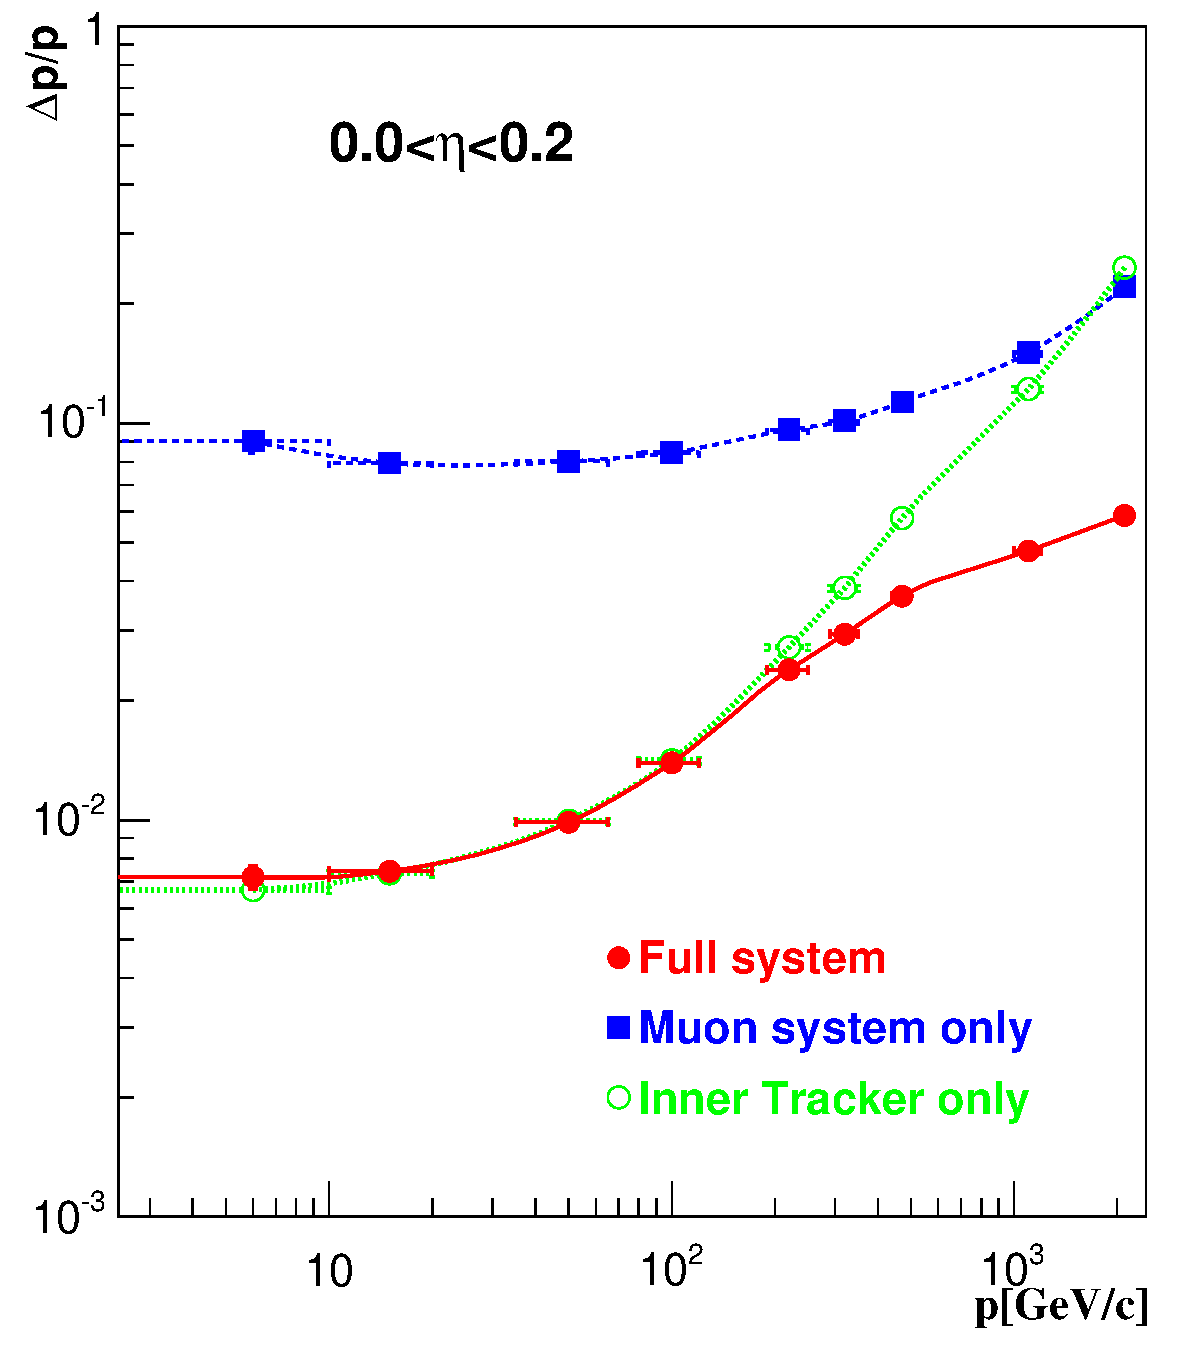
\includegraphics[width=\textwidth]{muon_barrel}
    \caption{Barrel.}
    \label{fig:muon_barrel}
  \end{subfigure}
  \begin{subfigure}{0.48\textwidth}
    \centering
    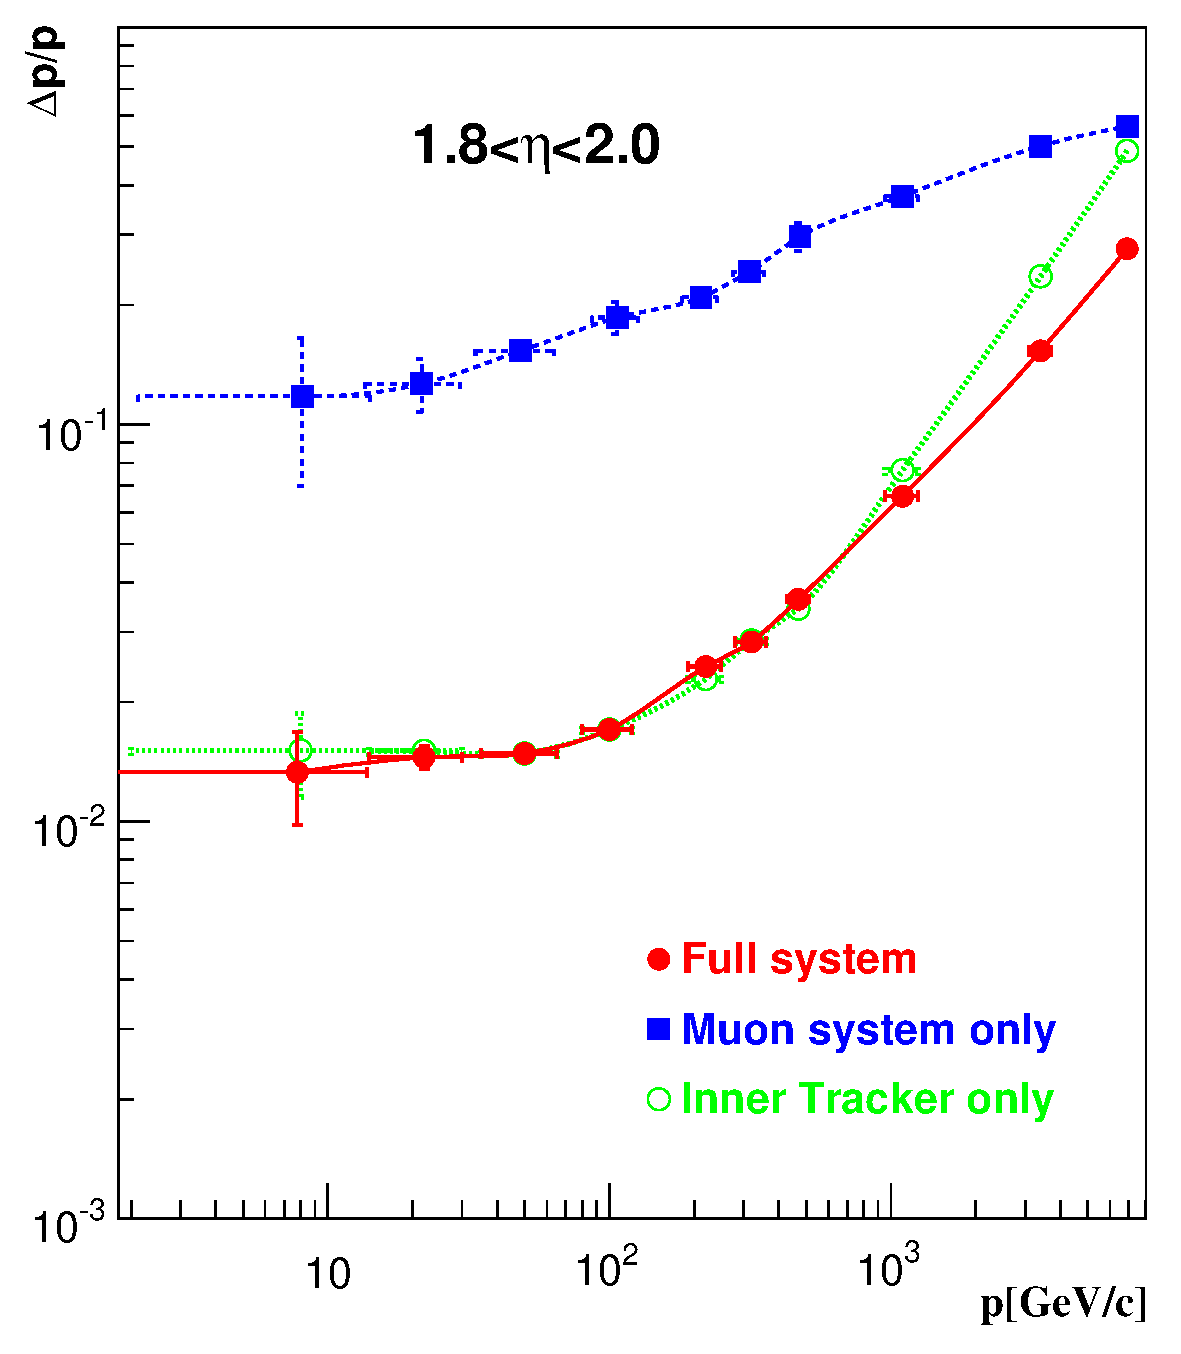
\includegraphics[width=\textwidth]{muon_endcap}
    \caption{Endcap.}
    \label{fig:muon_endcap}
  \end{subfigure}
  \caption[Muon transverse momentum resolution as a function of the muon
momentum.] {Muon transverse momentum resolution as a function of the muon
momentum using only the muon system, only the tracker and both, for barrel muons
($|\eta| < 0.2$) and endcap muons ($1.8<|\eta| < 2.0$). From
\cite{chatrchyan2008cms}.\label{fig:muon_performance}}
\end{figure}

\subsection{Trigger and Data Acquisition}
At design luminosity, the high bunch crossing frequency of the LHC means that
each crossing will contain an average of 20 superimposed inelastic
events every \unit{25}{\nano\second}, a rate of $10^{9}$ interactions per
second.
The size of an event is approximately \unit{1}{\mega\bel} after zero-suppression.
The total data output rate from CMS is $\approx \unit{80}{\tera\bel\per\second}$.
These figures are many orders of magnitude larger than the storage and offline
processing capability available to CMS, which corresponds to about
\unit{250}{\mega\bel\per\second} or about $\approx 10^{2}$ crossings written to the tape
storage every second. 

The vast majority of events will contain only glancing inelastic collisions and
may not be of interest from a physics perspective and can be discarded.  It is
the job of the trigger to reduce the rate of events by a factor of $10^6$ by
rejecting the uninteresting events while keeping as many interesting events as
possible.

An overview of the {DAQ} and trigger is shown in \FigureRef{fig:CMSDAQ}.
The trigger is separated into two parts; the Level-1 trigger and the High
Level Trigger.\cite{chatrchyan2008cms}

\begin{figure}[htbp]
  \centering
  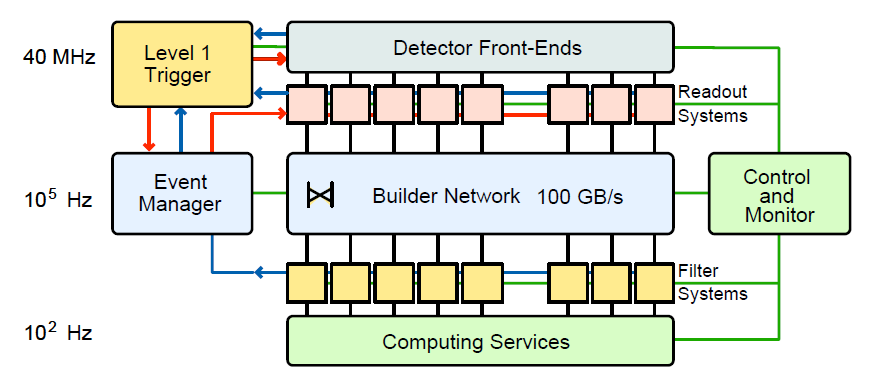
\includegraphics[width=0.85\textwidth]{CMSDAQ}
  \caption[Overview of the architecture of the CMS DAQ and trigger.] {Overview
of the architecture of the CMS DAQ and trigger. From \label{fig:CMSDAQ}
\cite{chatrchyan2008cms}.}
\end{figure}

\subsubsection{Level-1 Trigger}

The Level-1 trigger (L1) is designed to reduce the event rate from the bunch
crossing frequency of \unit{40}{\mega\hertz} to a maximum output rate of
\unit{100}{\kilo\hertz}.  The L1 trigger is implemented with custom-designed
fast programmable electronics that take as input coarse data from the
calorimeters and muon systems; the high resolution data are placed in pipe-lined
memories awaiting a Level-1 decision. The reduced resolution and granularity data are used to form ``trigger
primitives'', such as isolated high energy electromagnetic deposits that pass a
certain \PT or \ET threshold, upon which the L1 Trigger bases its decision. It
also receives information on event-wide variables such as the total sum of
transverse energy and the missing transverse energy.

\subsubsection{High-Level Triggers}
After a fixed time interval of \unit{3.2}{\micro\second} the high resolution
event data held in the pipeline memories are either read out or discarded
depending on the decision at the Level-1 trigger.  The data are transferred to a
processor running the high-level trigger software.

The high-level trigger (HLT) is a software system which runs on a server farm
with over one thousand commercial multicore processors with access to the
complete event data allowing it to make more complex calculations. 
Objects are reconstructed in the HLT as they are needed and events are discarded
as soon as possible to avoid wasting processing time.
The decision to accept an event is based on the requirements on the datasets
used in {CMS} analyses. A typical data-set requires a high \pT
HLT-reconstructed object or an amount of missing transverse energy in the event.
For example, the data-sets relevant to this thesis require a single high \pT
electron, as is described in \SectionRef{sec:trigger1} and
\SectionRef{sec:trigger2}.

\subsubsection{Computing}

The {CMS} data are available in several different file formats that contain
different levels of details \cite{grandi2004cms},
\begin{itemize}
\item Raw data, is the output of the events that pass the {HLT}. The files
contain the detector data, the {L1} trigger results, the {HLT} trigger
results and the higher-level objects that are created during the {HLT}
process.
\item Reconstructed (RECO) data, is the output of the reconstruction process.
The files contain the reconstructed physics objects and reconstructed hits and
clusters.
\item Analysis Object Data (AOD), is the reduced event representation and
contains only the reconstructed objects. This is the format that is used to
perform physics analyses.
\end{itemize}

CMS utilises a distributed computing model called the ``Grid''.  The Grid
consists of several clusters of computers distributed around the world and
organised into several tiers \cite{grandi2004cms}.  Events that pass the {HLT}
are sent to the primary Tier-0 centre where the raw data are stored on tape
before undergoing prompt reconstruction. The reconstructed data are distributed
to Tier-1 and Tier-2 centres at national laboratories and universities around the
world. The roles of the Tier-1 and Tier-2 sites are to run the physics analyses
and to reprocess the data when updated calibrations are available. This is
typically done once or twice a year.


  \chapter{W Bosons at the LHC}
\label{chap:wboson}

\PW boson production is an important process for physics studies at the LHC, not
only for accurate measurements of the Standard Model, but also as a background
to many processes from new physics. 
At the {LHC}, \PW bosons are produced at a high rate while offering a clean
experimental signal with a final state consisting of, in the case of a
leptonically decaying \PW, a single high \PT lepton with a large amount of
missing transverse energy due to the neutrino in the event. 
The production of \PW bosons provides important
information on the interacting partons within the colliding
hadrons\cite{catani,kom}.

This chapter will first describe the asymmetric production of \PWp and \PWm bosons.
The next section will describe the leptonic decay of the \PW and describe the electron
charge asymmetry observable. The final section will show some theoretical
predictions of the electron charge asymmetry.

\section{W Boson Production}

The dominant production process for a \PW boson at a proton-proton collider is
given in \EquationRef{wbos:wprod},
and shown in \FigureRef{wbos:wproddiag}. 
\begin{equation}
  h_1(p_1) + h_2(p_2)
  \to 
  \PW + X
  \to
  \Plepton \Pnue + X.
  \label{wbos:wprod}
\end{equation}
The \PW boson is produced in the collision of a quark and an anti-quark from the
two incoming protons, $h_1$ and $h_2$, with momenta $p_1$ and $p_2$\footnote{In
this thesis, $p_1 = p_2 = \unit{3.5}{\TeV}. $}.  $X$ represents the accompanying
final state.

\begin{figure}[htbp]
  \centering
  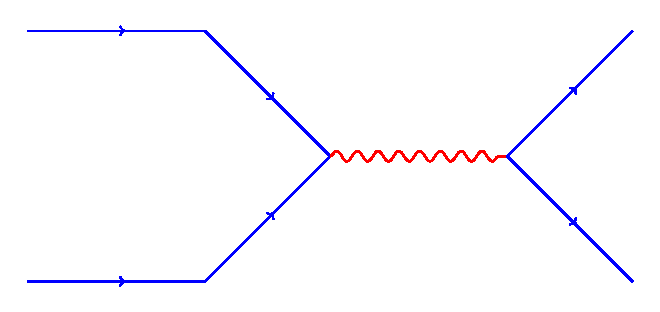
\includegraphics[width=0.6\textwidth]{w_production}
  \caption{Diagram of a W boson production and leptonic decay at a hadron-hadron collider.}
  \label{wbos:wproddiag}
\end{figure}

The \PW production cross section can given by the convolution of the cross
section at the parton level, and the parton distribution functions (PDF) of the
protons,
\begin{multline}
  d\sigma_{(\HepProcess{h_1 h_2 \to \PWpm})}(p_1,p_2;Q^{2}) = \\
  \sum\limits_{a,b}
  \int_0^1 \! \mathrm{d} x_1 
  \int_0^1 \! \mathrm{d} x_2 
  f_a^{h_1}(x_1,Q^2)
  f_b^{h_2}(x_2,Q^2) 
  d\hat{\sigma}_{(\HepProcess{a b \to \PWpm})}(x_1 p_1, x_2 p_2; Q^2),
  \label{wbos:xsec}
\end{multline}
where $\sum\limits_{a,b}$ represents the sum over the initial parton states $a$
and $b$, $f_a^{h}(x,Q^2)$ represents the proton {PDF} and
$d\hat{\sigma}_{(\HepProcess{a b \to \PWpm})}(x_1 p_1, x_2 p_2; Q^2)$
represents the partonic sub-process cross section. The ability to separate the
complicated QCD process in to a short-range perturbatively-calculable
hard-scattering process and long-range experimentally-measurable parton
densities is given by factorisation theorems. 
\todo{not sure this is enough}

\subsubsection*{Partonic Sub-Process}

At leading order (LO) the process for a \PWp is
\begin{equation}
  \HepProcess{\Pup + \APdown \to \PWp \to \Pleptonplus \Pnulepton} 
  \label{wbos:wpprod} 
\end{equation}
and for a \PWm:
\begin{equation}
  \HepProcess{\APup + \Pdown \to \PWm \to \Pleptonminus \APnulepton}
  \label{wbos:wmprod} 
\end{equation}
Tree-level Feynman diagrams representing these processes are shown in
\FigureRef{fig:w_process}.
At the {LHC} (a proton-proton collider), one parton is most to likely be a
valence quark with a high fraction of the proton's momentum, and the other
parton will tend to be a sea anti-quark with a lower fraction of the momentum
than the quark. The difference in momentum of the partons causes the \PW bosons 
to tend to be produced at high rapidities. 

\begin{figure}[htbp]
  \centering
  \begin{subfigure}{0.45\textwidth}
    \centering
    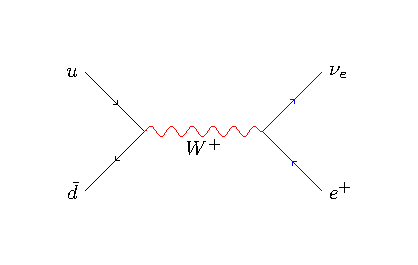
\includegraphics[width=\textwidth]{w_process_wp}
    \caption{\HepProcess{\Pup + \APdown \to \PWp \to \Pleptonplus \Pnulepton}}
    \label{fig:w_process_wp}
  \end{subfigure}
  \begin{subfigure}{0.45\textwidth}
    \centering
    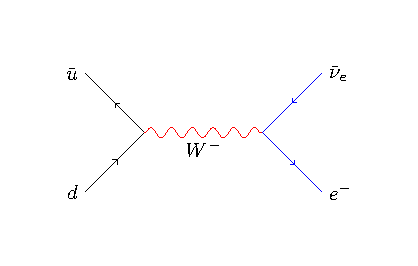
\includegraphics[width=\textwidth]{w_process_wm}
    \caption{\HepProcess{\APup + \Pdown \to \PWm \to \Pleptonminus \APnulepton}}
    \label{fig:w_process_wm}
  \end{subfigure}
  \caption{Tree-level diagrams for \PWp and \PWm boson production and electron
decay at a hadron-hadron collider.}\label{fig:w_process} 
\end{figure}

\subsubsection*{Proton Parton Distribution Function} 
The proton PDF represents the number density of
parton $a$ that has a fraction between $x$ and $x+\mathrm{d}x$ of the
momentum of the colliding hadron $h$ at a resolution scale $Q^{2}$.

\begin{figure}[htbp]
  \centering
  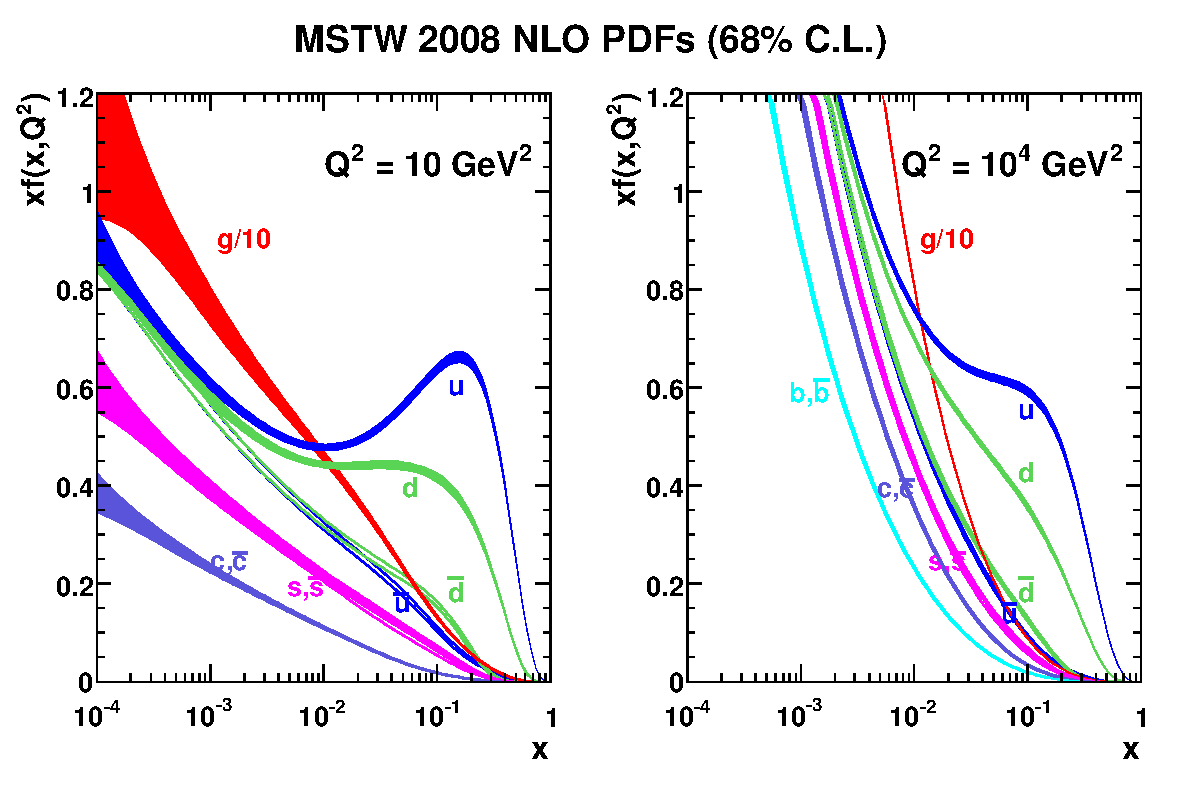
\includegraphics[width=\textwidth]{mstw2008nlo68cl_allpdfs}
  \caption
[Proton PDFs at $Q^2 = 10\ \GeV^2$ and $Q^2 = 10^{4}\ \GeV^2$.]
{Proton PDFs at $Q^2 = 10\ \GeV^2$ (left) and $Q^2 = 10^{4}\ \GeV^2$ (right) from \cite{martin2009parton}.}
  \label{wbos:pdf}
\end{figure}

The {PDFs} are obtained from global fits to experimental data
\cite{martin2009parton}.  \FigureRef{wbos:pdf} (right) shows the proton PDF at
$Q^2\approx M_{\PW}^2$ from the MSTW group.  The anti-quark parton densities
$\APup(x,Q^2)$ and $\APdown(x,Q^2)$ are relatively similar especially at the LHC
energies, where the parton momentum fraction, x, tends to be small.
However, the {PDF} for the valence quarks in the proton differ, 
the up-type quark dominates over the down-type quark.
This is due to the excess of up-type valence quarks with respect to down-type
valence quarks in the proton (\HepProcess{\Pup\Pup\Pdown}). 
This can be seen in the ratio of the up-type and the down-type {PDFs},
\begin{equation}
  R_{ud}(x,Q^2) = \frac{\Pup(x,Q^2)}{\Pdown(x,Q^2)} > 1,
\end{equation}
where $\Pup(x,Q^2)$ are the up and down quark {PDFs}.
\FigureRef{fig:pdf_plots} shows the ratio of the up-type and down-type quarks.
The ratio $R \approx 1$ for $x \ll 1$. This is due to the equal number or
up-type and down-type sea quarks in the proton. The equal number of sea quarks,
and the unequal number of valence quarks has the effect that if an up-type quark
is picked at random from the proton, it is more likely to be a higher momentum
valence quark, than if a down-type quark is picked.  Therefore, an up-type quark
will tend to have a greater fraction of the proton's momentum than a down-type
quark.

\begin{figure}[htbp]
  \centering
  %\begin{subfigure}{\textwidth}
    %\centering
    %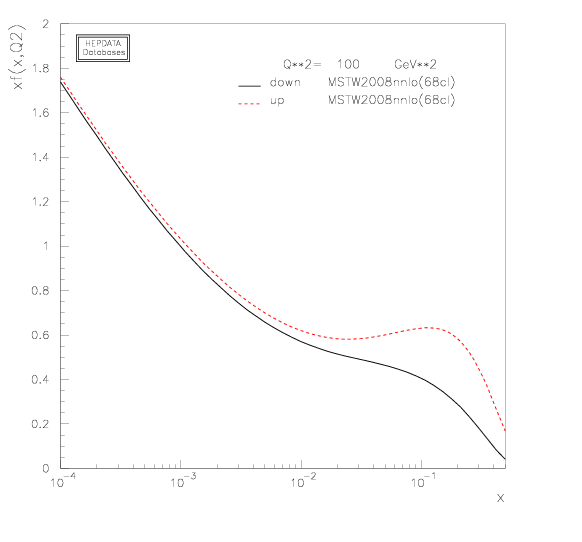
\includegraphics[width=0.75\textwidth]{plot_pdf}
    %\caption{PDF for \Pup and \Pdown}
    %\label{fig:plot_pdf}
  %\end{subfigure}
  %\begin{subfigure}{\textwidth}
    %\centering
    %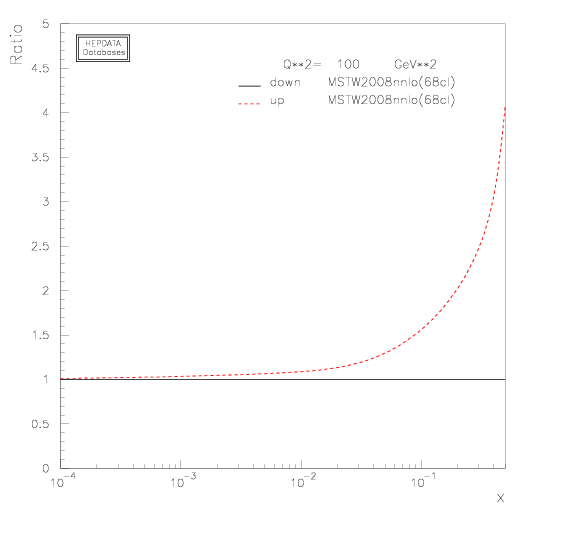
\includegraphics[width=0.75\textwidth]{plot_pdf_ratio}
    %\caption{Ratio for \Pup and \Pdown PDF}
    %\label{fig:plot_pdf_ratio}
  %\end{subfigure}
  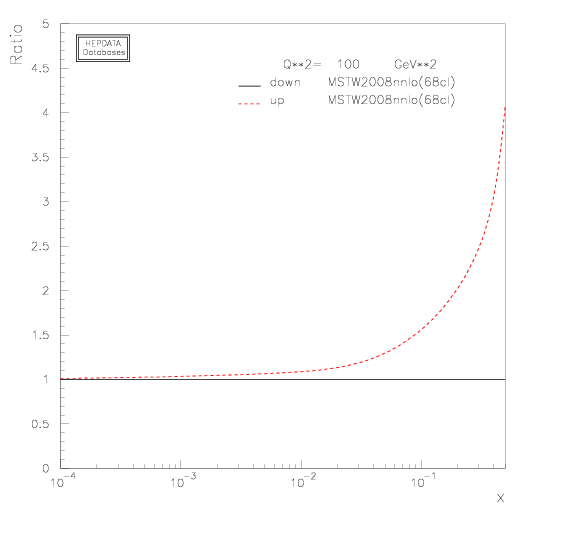
\includegraphics[width=0.75\textwidth]{plot_pdf_ratio}
  \caption[Ratio of up quarks to down quarks, $R_{ud}$ at $Q^2=\unit{100}{\GeV^2}$.] 
{Ratio of up quarks to down quarks, $R_{ud}$ at $Q^2=\unit{100}{\GeV^2}$.  Generated from \cite{hepdata} using the MSTW2008nlo
PDF sets \cite{martin2009parton}.}
  \label{fig:pdf_plots} 
\end{figure}

\subsection{\PW Boson Rapidity Distribution}
\label{wbos:wrapsec}

The rapidity of a particle is defined as,
\begin{equation}
    y = \frac{1}{2} \ln \left(\frac{E+p_\text{L}}{E-p_\text{L}}\right),
\end{equation}
where $p_{L}$ is the longitudinal component (the component along the beam axis)
of the momentum of the particle. It represents the boost along the beam axis
required to go from the lab frame to the frame where the particle is produced
perpendicular to the beam axis.
\begin{figure}[htbp]
  \centering
  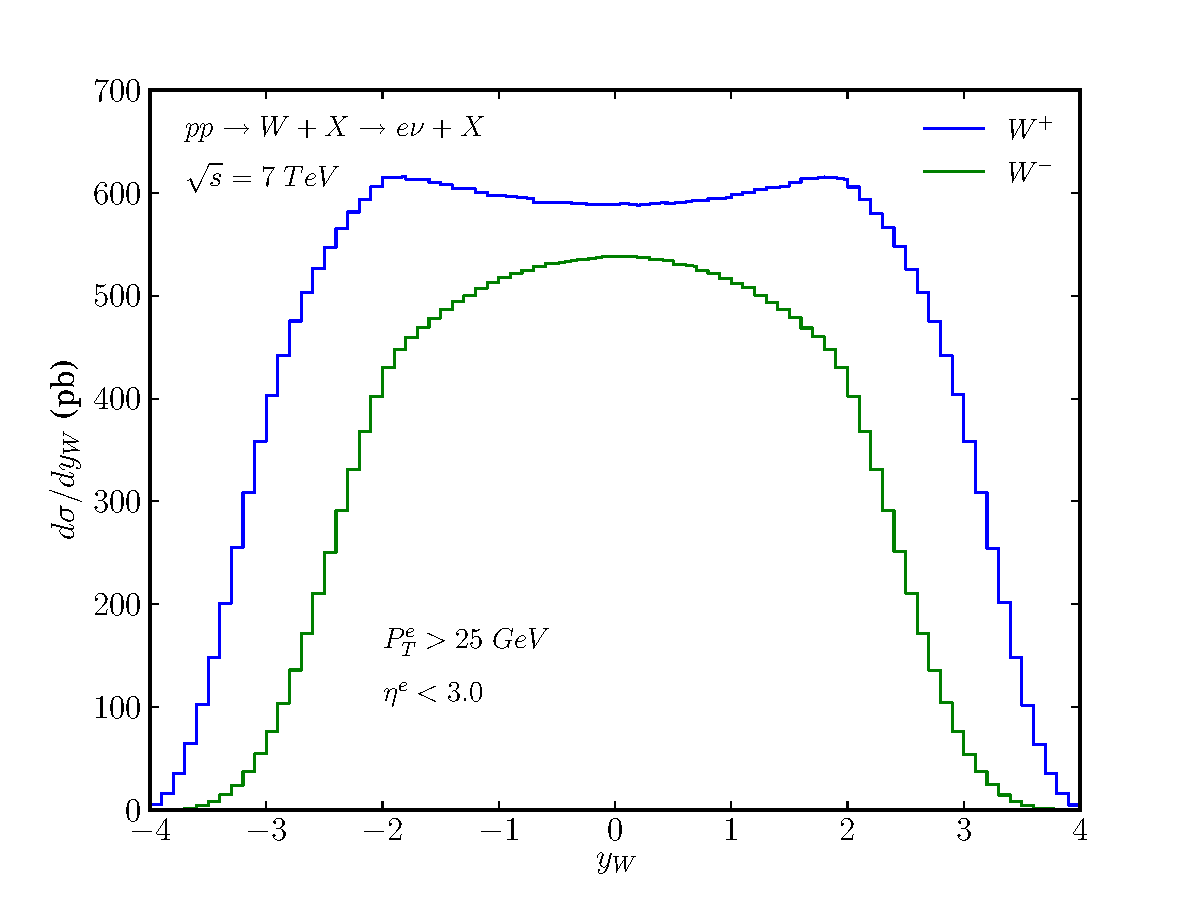
\includegraphics[width=0.8\textwidth]{w-rapidity}
  \caption[The rapidity distribution for \PWp and \PWm bosons in
${\sqrtS=\unit{7}{\TeV}}$ proton-proton collisions at the LHC.] {The rapidity
distribution for \PWp and \PWm bosons in $\sqrtS=\unit{7}{\TeV}$ proton-proton
collisions at the LHC.  Generated with the MSTW2008nlo
PDF set\cite{martin2009parton} interfaced with the MCFM generator tool \cite{campbellmcfm}.}
  \label{wbos:wrapid}
\end{figure}

The rapidity distributions, $y_W$, for \PWp and \PWm bosons produced at the
{LHC} are shown in \FigureRef{wbos:wrapid}.  The \PWp cross section is greater
than the \PWm cross section.  This is a consequence of the different production
processes for \PWp and \PWm bosons (shown in \EquationRef{wbos:wpprod} and
\EquationRef{wbos:wmprod} respectively) and the {PDF} for the valence quarks in
the proton differing as seen in \FigureRef{fig:pdf_plots}. The up-type quark
{PDF} dominates over the down-type which leads to a greater \PWp production rate
than \PWm.

It is also seen in \FigureRef{wbos:wrapid} that the \PWm tends to be produced
more centrally whereas the \PWp can be produced at larger rapidities. This is due
to up-type quarks tending to carry a greater fraction of the proton's momentum,
$x$, than the down-type quarks as seen in \FigureRef{fig:pdf_plots}.

The momentum fraction, $x$, of the interacting quarks is correlated with the
rapidity of the \PW boson. Therefore, the ratio of $\Pup$ and $\Pdown$ quarks as
a function of momentum fraction, $x$, is directly related to the difference in
the \PWp and \PWm production cross sections as a function of the boson rapidity.

Therefore a measurement of the asymmetric production of \PW bosons, as a
function of the rapidity of the boson, at the {LHC} provides important
information on the ratio of the up-type and down-type quark parton densities as
a function of $x$ ($R_{ud}(x,Q^2)$) within the proton\cite{kom}. 

\subsection{\PW Boson Charge Asymmetry}

The \PWpm boson charge asymmetry is defined as,
\begin{equation}
  A_{W}(y_{\PW})=
    \frac{ 
      \nicefrac{ d\sigma (\PWp) }{ dy_{W} } -
      \nicefrac{ d\sigma (\PWm) }{ dy_{W} }
    }
    {
      \nicefrac{ d\sigma (\PWp) }{ dy_{W} } +
      \nicefrac{ d\sigma (\PWm) }{ dy_{W} }
    }
,
\label{wbos:wasym}
\end{equation} 
where $y_{W}$ is the boson rapidity, and 
$\nicefrac{ d\sigma (\PWpm) }{ dy_{W} }$ is the \PWpm production cross section
at a fixed $y_{W}$.  
If $d\sigma(\PWp) > d\sigma(\PWm) $ then $A_{W}(y_{\PW})> 0$,
else if $d\sigma(\PWp) < d\sigma(\PWm) $ then $A_{W}(y_{\PW})< 0$,
and for symmetric \PWpm boson production, $A_{W}(y_{\PW})= 0$,

The prediction for the W boson charge asymmetry as a function of the boson
rapidity is shown in \FigureRef{wbos:chargeasym}. $A_{W}(y_{\PW})> 0$ and
increases as the rapidity increases.

\begin{figure}[htbp]
  \centering
  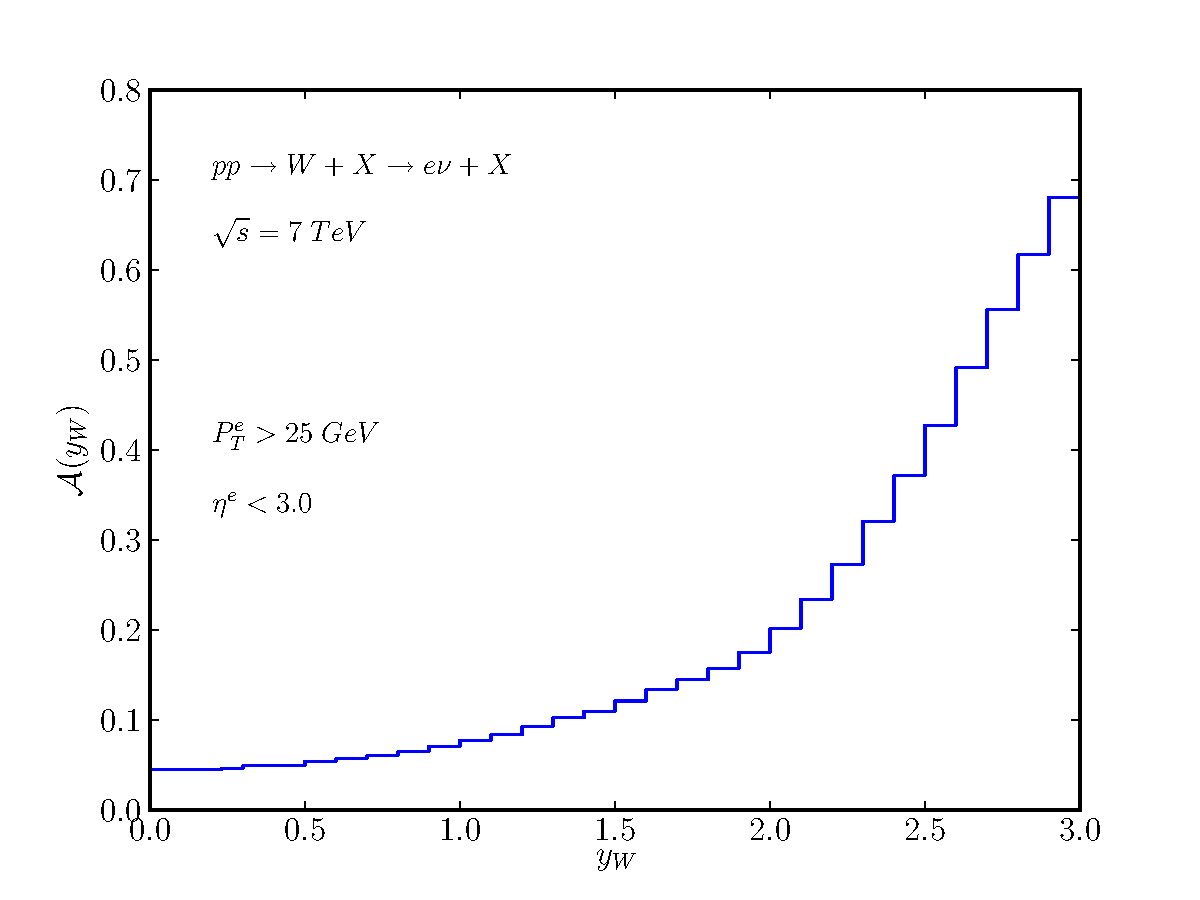
\includegraphics[width=0.8\textwidth]{w-asym}
  \caption[\PW boson charge asymmetry at LHC in ${\sqrtS=\unit{7}{\TeV}}$
proton-proton collisions.] {\PW boson charge asymmetry at LHC in
$\sqrtS=\unit{7}{\TeV}$ proton-proton collisions.  Generated with the
MSTW2008nlo PDF set\cite{martin2009parton} interfaced with the and the MCFM
generator tool \cite{campbellmcfm}.}
  \label{wbos:chargeasym}
\end{figure}

\PW bosons are identified by their decay to a lepton plus neutrino, however at
hadronic colliders the neutrino longitudinal momentum cannot be determined
which means that the \PW rapidity, $y_{W}$, cannot be measured.  Instead what
is studied is the charge asymmetry in the leptons that result from the \PW boson
decaying leptonically.

%It is possible to overcome the difficulty in determining the boson rapidity
%by extrapolating the neutrino longditudinal momentum from the lepton neutrino
%with a {MC} study. 

\section{W Boson Decay}
The \PW boson will decay to either a lepton and neutrino, or a pair of up and
down quarks. The branching fractions for the various decays are shown in
\TableRef{tab:w_decay}.
This thesis will consider the electron decay of the \PW boson which will occur
in approximately $11\%$ of \PW boson decays.

\begin{table}[htbp]
\begin{center}
\begin{tabular}{l l }
\toprule
\PWp Decay Mode & Fraction ($\Gamma_{i}/\Gamma$)\% \\
\midrule
\APelectron\Pnu & $10.75\pm0.13$ \\
\APmuon\Pnu     & $10.57\pm0.15$ \\
\APtauon\Pnu    & $11.25\pm0.20$ \\
hadrons         & $67.60\pm0.27$ \\
\bottomrule
\end{tabular}
\caption[Experimentally measured \PWp decay modes.] {Experimentally measured
\PWp decay modes. The decay modes of \PWm are the charge conjugates of the \PWp.
From \cite{beringer2012review}.\label{tab:w_decay}} 
\end{center}
\end{table}

\subsection{Electron Pseudorapidity Distribution}
The rapidity distributions of the charged leptons produced from \PWpm decay are
further complicated by the charge asymmetric decay of the \PWpm boson. 
The asymmetric decay arises due to the $V-A$ coupling of the \PW boson to the
annihilating \HepProcess{\Pquark\APquark} pair and the decaying lepton pair.

At leading order (LO) the \PWp is produced in the annihilation of a \Pup valance quark
with a \APdown sea-quark (\EquationRef{wbos:wpprod}). 
If the parton masses are neglected the \Pup is left-handed and the \APdown is
right-handed, as shown at the top of \FigureRef{wbos:wspin}. 

In the \PWp decay the \Ppositron is right-handed and the \Pnue is left-handed.
\FigureRef{wbos:wspin} shows that if the  positron is produced in the same direction
as the incoming \APdown quark angular momentum is conserved and the decay is
allowed.
However the decay where the positron is produced in the same direction as the
incoming \Pup quark is forbidden.
A similar argument holds true for \PWm decays, where the \Pelectron is produced
preferentially in the direction of the \Pdown quark.

\begin{figure}[htbp]
  \centering
  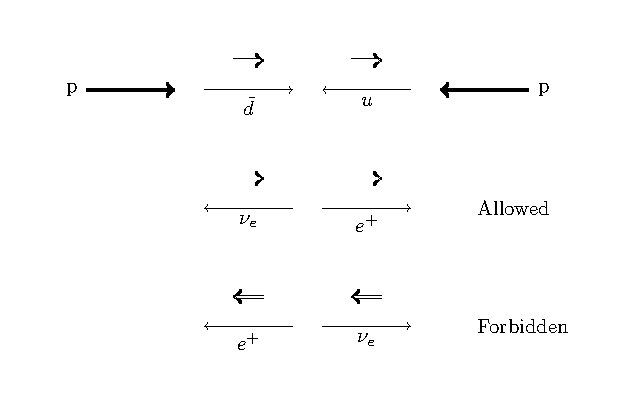
\includegraphics[width=0.8\textwidth]{w_decay_directions}
  \caption[Preferred directions of electron spins in
\HepProcess{\PWplus\to\APelectron\Pnue} decay.] {Preferred directions of
electron spins in \HepProcess{\PWplus\to\APelectron\Pnue} decay.  The heavy
arrows show the directions of the incoming protons, the thin arrows show the
directions of the incoming quarks and the outgoing electron and neutrino. The
double arrows show the spins.  Modified from \cite{aitchison2004gauge}. }
  \label{wbos:wspin}
\end{figure}

The distribution of the electron from \PWpm decay in the massless limit
is given by\cite{perkins2000introduction,aitchison2004gauge},
\begin{equation}
  \frac{1}{\sigma_{u\bar{d}}}
  \frac{d \sigma_{u\bar{d}}}{d \cos \theta_{\Plepton d}^{\ast}}
  =
  \frac{1}{\sigma_{d\bar{u}}}
  \frac{d \sigma_{d\bar{u}}}{d \cos \theta_{\Plepton d}^{\ast}}
  \propto
  (1+\cos \theta_{\Plepton d}^{\ast})^2
  \label{wbos:lepton}
\end{equation}
where $\theta_{\Plepton d}^{\ast}$ is the scattering angle of the charged
lepton with respect to the direction of the down-type quark or anti-quark, in
the centre of mass system of the two quarks. The cross section is maximised when
$\theta_{\Plepton D}^{\ast}$ is minimised and the charged lepton is produced in
the same direction as the down-type quark.

The rapidity distribution of the electron is therefore a convolution of the
{electroweak} correlations in \EquationRef{wbos:lepton} with the \PW rapidity
described in \SectionRef{wbos:wrapsec}.  In proton-proton collisions the \PWp
tends to be produced in the direction of the \Pup.  However, due to the
electroweak correlations the charged lepton from the decaying \PWp will tend to
be produced along the direction of the down-type quark and therefore will shift
the rapidity distribution of the lepton to be more central. Similarly, \PWm
bosons tend to be produced more centrally, however the electroweak correlations
will shift the charged lepton rapidity distribution to higher rapidities.

\FigureRef{fig:leptonrapidity} shows the Monte Carlo (MC) generated
pseudorapidity distribution of electrons and positrons produced in
$\sqrtS=\unit{7}{\TeV}$ proton-proton collisions.  
The pseudorapidity is defined as 
\begin{equation}
    \eta = -\ln\left[\tan\left(\frac{\theta}{2}\right)\right], 
\end{equation}
where $\theta$ is the polar angle.  In the massless approximation, the
pseudorapidity of the electron is equal to the rapidity.

\begin{figure}[htbp]
  \centering
  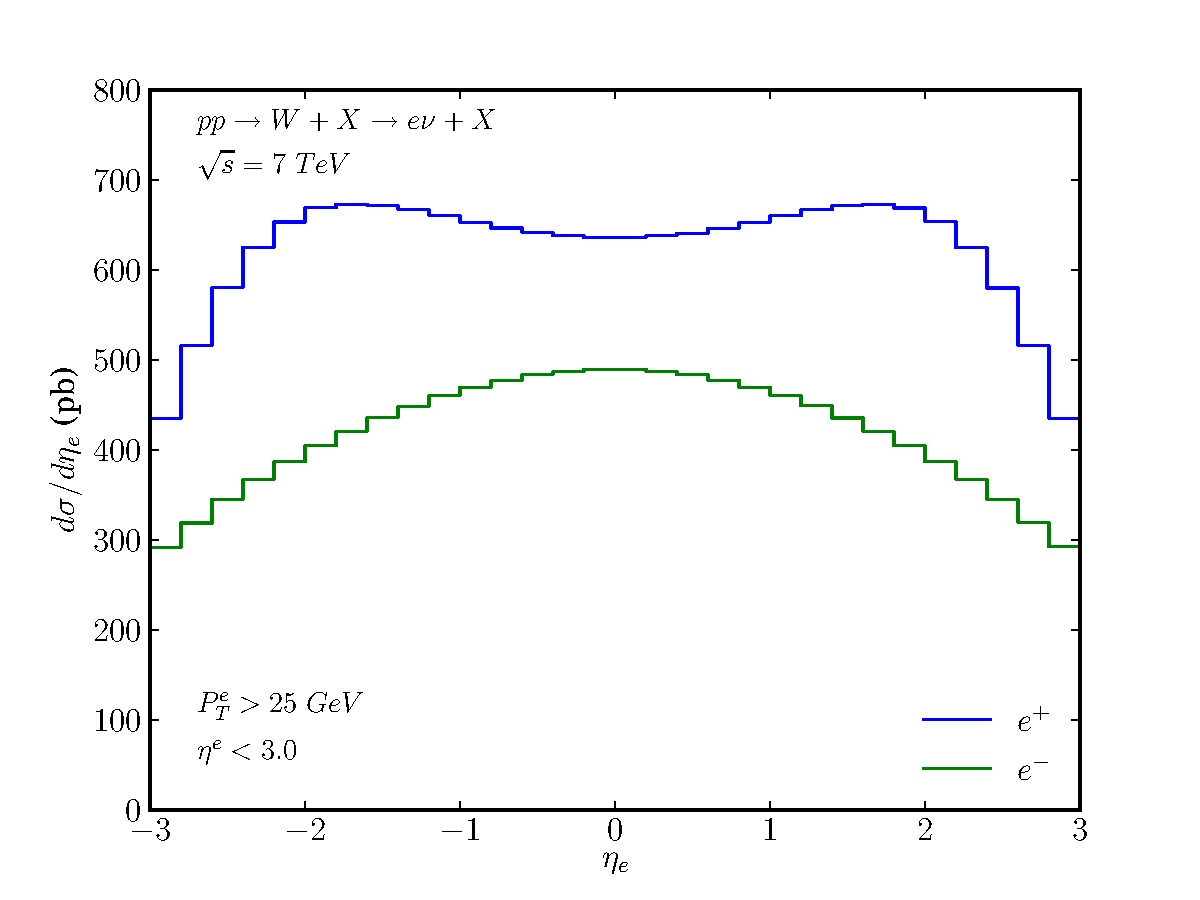
\includegraphics[width=0.8\textwidth]{lepton-rapidity}
  \caption[Electron and positron pseudorapidity, $\eta_e$, distributions in
$\sqrtS=\unit{7}{\TeV}$ proton-proton collisions.] {Electron and positron
pseudorapidity, $\eta_e$, distributions in $\sqrtS=\unit{7}{\TeV}$ proton-proton
collisions. Generated with the MSTW2008nlo PDF set\cite{martin2009parton}
interfaced with the MCFM generator tool \cite{campbellmcfm}.}
  \label{fig:leptonrapidity}
\end{figure}

\subsection{Electron Charge Asymmetry}

The electron asymmetry is defined in \EquationRef{eq:AsymThe} analogously to the
\PW boson asymmetry in \EquationRef{wbos:wasym}, as the difference in the
\HepProcess{\PWplus \to \APelectron} and \HepProcess{\PWminus \to \Pelectron}
over the total \inclusiveWe cross section.
\begin{equation}
A_{the}(\eta)=\frac
  { \frac{d\sigma}{d\eta}(\Wpenu) - \frac{d\sigma}{d\eta}(\Wmenu) }
  { \frac{d\sigma}{d\eta}(\Wpenu) + \frac{d\sigma}{d\eta}(\Wmenu) }
\label{eq:AsymThe}
\end{equation} 

The electron charge asymmetry has previously been studied in $p\bar{p}$
collisions by the CDF and D0 experiments at the Fermilab Tevatron collider
\cite{cdfWAsym,d0WAsym}. 

\FigureRef{wbos:asym_simple} shows the electron charge asymmetry prediction for
electron transverse momentum cuts of \unit{25}{\GeV}. The prediction was
produced using the MSTW2008NLO PDF\cite{martin2009parton} set.
Unlike the \PW asymmetry, the electron asymmetry turns over at $\eta\approx
2.25$. This effect is due to the electroweak correlations in the leptonic decay of
the \PW boson.

\begin{figure}[htbp]
  \centering
  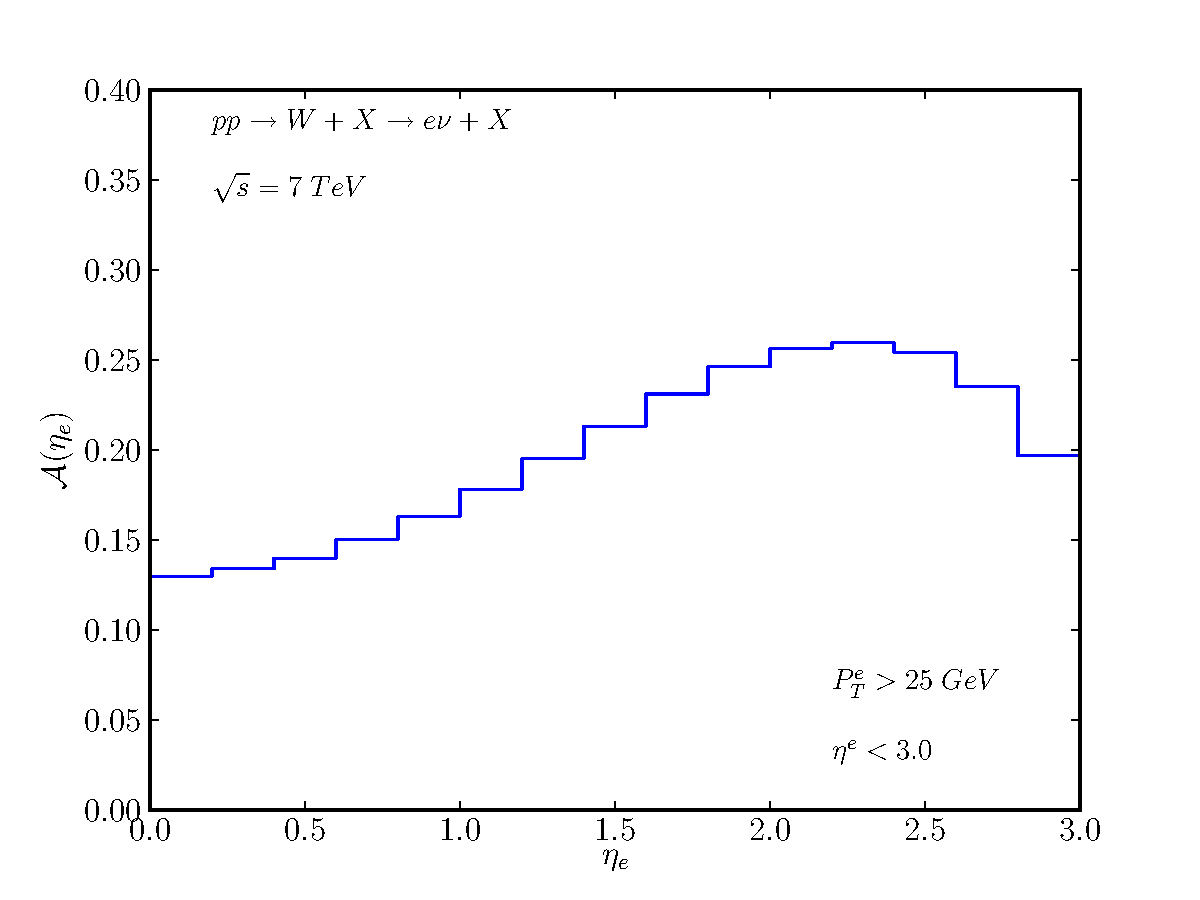
\includegraphics[width=0.8\textwidth]{lepton-asym}
  \caption[Electron charge asymmetry at LHC in ${\sqrtS=\unit{7}{\TeV}}$
proton-proton collisions.] {Electron charge asymmetry at LHC in
$\sqrtS=\unit{7}{\TeV}$ proton-proton collisions.  Generated with the
MSTW2008nlo PDF set\cite{martin2009parton} interfaced with the MCFM generator tool
\cite{campbellmcfm}.}
  \label{wbos:asym_simple}
\end{figure}

In an experiment, the cross section is not measured directly, instead what is
measured are the electron and positron yields.  The experimentally measured
asymmetry is given by \EquationRef{eq:AsymExp},
\begin{equation}
A_{exp}(\eta)=\frac{  \frac{dN}{d\eta}(\APelectron) -
\frac{dN}{d\eta}(\Pelectron)}{\frac{dN}{d\eta}(\APelectron) +
\frac{dN}{d\eta}(\Pelectron)}
\label{eq:AsymExp}
\end{equation} 

To get from the experimentally measured asymmetry to the lepton charge
asymmetry, \EquationRef{eq:NumEve} must be used, which takes into
account the experimental effects such as the luminosity (${\cal L}$), high
level trigger ($\epsilon_{HLT}$), offline efficiency ($ \epsilon_{off}$) and
the acceptance ($\epsilon_{acc}$).

\begin{equation}
\frac{dN}{d\eta} = {\cal L } \frac{d\sigma}{d\eta}  \epsilon_{HLT}
\epsilon_{off} \epsilon_{acc}
\label{eq:NumEve}
\end{equation} 
As the asymmetry is a ratio, the luminosity, high level trigger and the
offline efficiency can be cancelled out assuming that they are not asymmetric
with respect to charge. 

The acceptance cannot be cancelled, it is a function of transverse momentum of
the electron, and these distributions will differ for \Pelectron and \APelectron.
A correction due to acceptance effect could be included, but would be highly
dependent on the choice of PDF set used to generate the corrections \cite{cdfWAsym}.
The measurements presented in this thesis do not correct for acceptance effects.

%\begin{align} 
%A_{exp}(\eta) &= \frac{ \frac{dN}{d\eta}(\Pelectron) -
%\frac{dN}{d\eta}(\APelectron) }{\frac{dN}{d\eta}(\Pelectron) +
%\frac{dN}{d\eta}(\APelectron) }\\   
              %&= \frac{ \frac{d\sigma}{d\eta}(\Wpenu) -
%\frac{\epsilon^{-}_{acc}}{\epsilon^{+}_{acc}} \frac{d\sigma}{d\eta}(\Wmenu) }{
%\frac{d\sigma}{d\eta}(\Wpenu) + \frac{\epsilon^{-}_{acc}}{\epsilon^{+}_{acc}}
%\frac{d\sigma}{d\eta}(\Wmenu) }
%\label{eq:AsymExpCorr}
%\end{align}

\section{ Theoretical Predictions of the Electron Charge Asymmetry }
\label{sec:asymuncert}

In this section predictions for the electron charge asymmetry are investigated in
detail.  The predictions are calculated using the MCFM\cite{campbellmcfm} {MC} tool
interfaced with the LHAPDF package\cite{whalley2005houches}.  LHAPDF provides an
interface to many different {PDF} sets. For the following predictions, PDF sets from
the MSTW \cite{martin2009parton} and CTEQ \cite{lai2010vv} collaborations are
used.

Corrections for final state radiation (FSR) are not included in the predictions.
In the measurements presented in the later chapters, FSR in considered as an
additional contribution to the electron energy resolution and is corrected for, so the
comparison of the measured asymmetry to the theoretical predictions is valid.

\subsection{Uncertainty on Theoretical Predictions}
The theoretical predictions of the electron charge asymmetry will have an error
associated with the uncertainty on the {PDF}.
The uncertainty on the {PDF} originates from the experimental errors on the
data used in the global fits performed by each of the {PDF} collaborations.

Each {PDF} collaboration produces a set of {PDFs} that include the
central value, or best fit to experimental data, and $2N$ error {PDFs}, where
$N$ is the number of free parameters used in the global
fit\cite{Bourilkov:2006cj}.
For each of the free parameters there is a PDF produced with the parameter at its upper
error and another with the parameter at its lower error. 

The uncertainty on the observable, in this case the lepton asymmetry, is found
by producing $2N+1$ theoretical predictions, one for each member of the {PDF}
set. The predictions are then used to approximate the {PDF} uncertainty by
using the `master equation'\cite{Bourilkov:2006cj,campbell2006hard}.
For the upper uncertainty,

\begin{equation}
\Delta A^{+}_{max}
= \sqrt{ \sum^{N}_{i=1} \left[ max( A^{+}_i-A_{0}, A^{-}_i-A_{0}, 0 ) \right]^{2}}
\end{equation}
and for the lower uncertainty,
\begin{equation}
\Delta A^{-}_{max}
= \sqrt{ \sum^{N}_{i=1} \left[ max( A_{0}-A^{+}_i, A_{0}-A^{-}_i, 0 ) \right]^{2}}
\end{equation}
where $A^{\pm}_{i}$ is the asymmetry prediction using the {PDF} with the
positive/negative fluctuation of parameter $i$ and $A_{0}$ is the prediction
using the central value.

\subsection{Prediction of the Electron Charge Asymmetry above \unit{25}{\GeV}}

\begin{figure}[htbp]
  \centering
  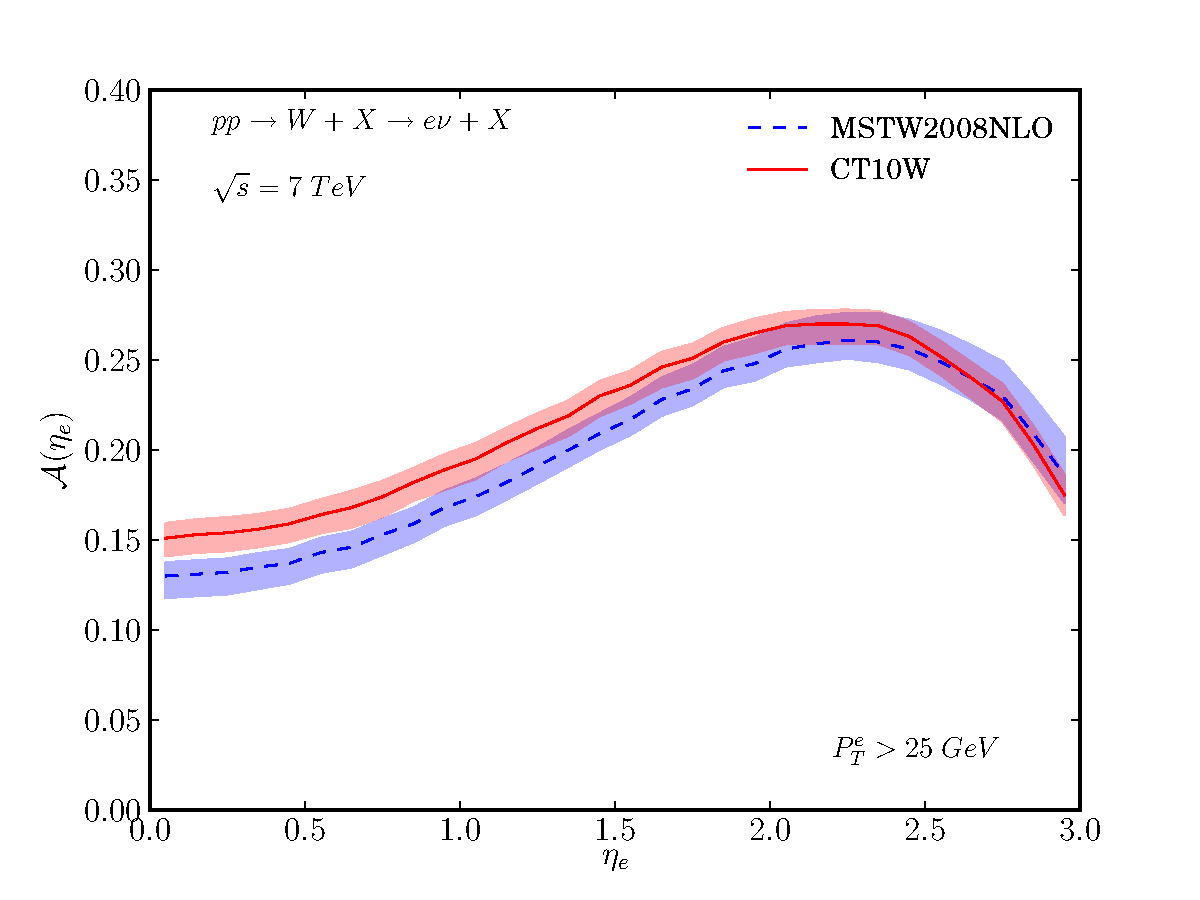
\includegraphics[width=0.8\textwidth]{asym-uncert}
  \caption[The theoretical electron charge asymmetry for a ${\pT>\unit{25}{\GeV}}$
with the {PDF} uncertainties.] {The theoretical electron charge
asymmetry\cite{monchenault2011predictions} for a $\pT>\unit{25}{\GeV}$ with the
{PDF} uncertainties for the MSTW08NLO\cite{martin2009parton} and
CT10W\cite{lai2010vv} {PDF} sets. The uncertainties are $68\%$ confidence level. The
predictions are generated using the {MCFM} \cite{campbellmcfm} generator.}
  \label{fig:asym-uncert}
\end{figure}

\FigureRef{fig:asym-uncert} shows the theoretical predictions for the electron
charge asymmetry for $\pT>\unit{25}{\GeV}$ with PDF sets from the MSTW
collaboration\cite{martin2009parton} and the CTEQ collaboration\cite{lai2010vv}.
The uncertainty due to the PDFs is included.  The predictions show a
disagreement at low rapidities. The CTEQ prediction tends to be higher and the
MSTW prediction lower. The disagreement is greater than the PDF uncertainty on
the prediction.

\subsection{Prediction of the Electron Charge Asymmetry above \unit{30}{\GeV}}

\begin{figure}[htbp]
  \centering
  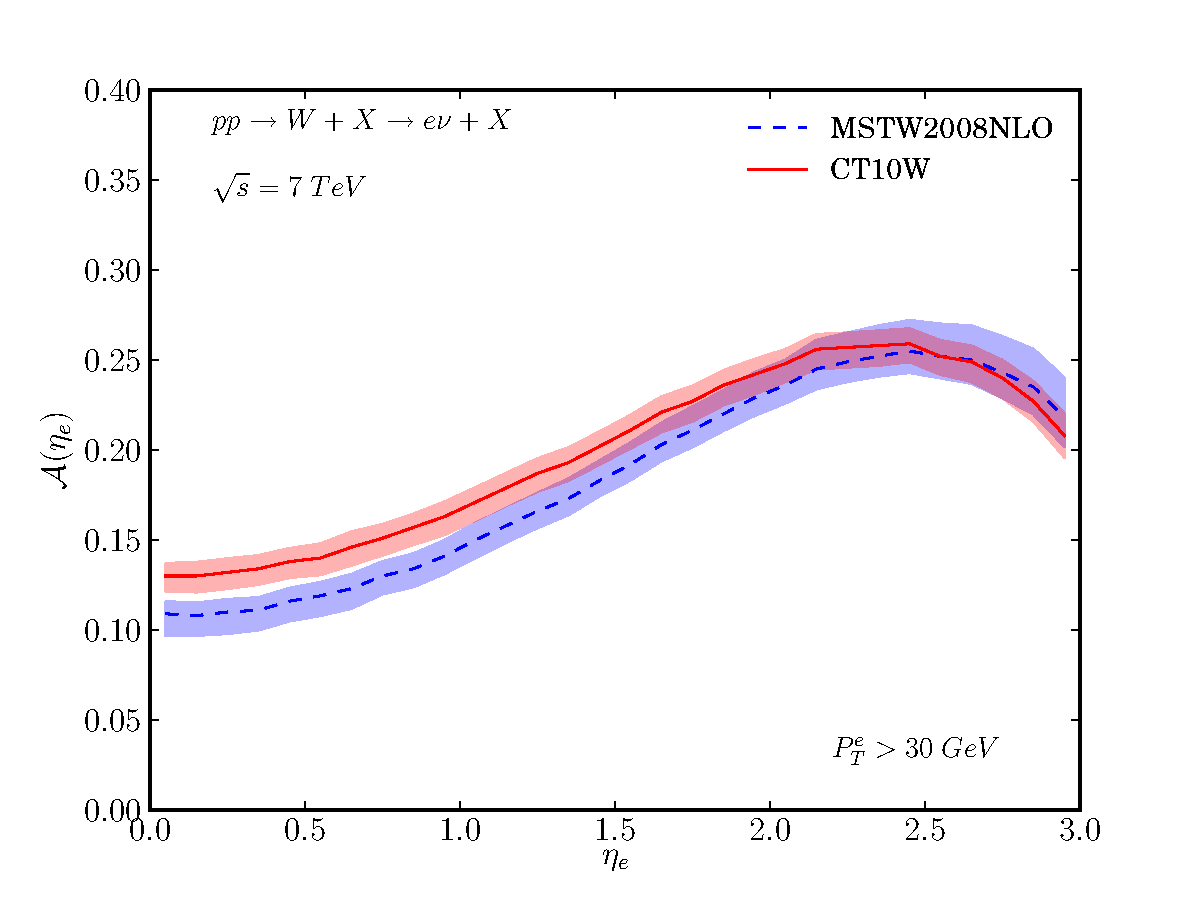
\includegraphics[width=0.8\textwidth]{asym-uncert-30}
  \caption[The theoretical electron charge asymmetry for a ${\pT>\unit{25}{\GeV}}$
with the {PDF} uncertainties.] {The theoretical electron charge
asymmetry\cite{monchenault2011predictions} for a $\pT>\unit{30}{\GeV}$ with the
{PDF} uncertainties for the MSTW08NLO\cite{martin2009parton} and
CT10W\cite{lai2010vv} {PDF} sets. The uncertainties are $68\%$ confidence level. The
predictions are generated using the {MCFM} \cite{campbellmcfm} generator.}
  \label{fig:asym-uncert-30}
\end{figure}

\FigureRef{fig:asym-uncert-30} shows the theoretical predictions for the
electron charge asymmetry for $\pT>\unit{30}{\GeV}$ with PDF sets from the MSTW
collaboration\cite{martin2009parton} and the CTEQ collaboration\cite{lai2010vv}.
Similar disagreement between the predictions at low rapidities is seen.

The asymmetry prediction at low rapidities is lower than the prediction with an
electron cut at \unit{25}{\GeV}. The turning point in the asymmetry is also
shifted to higher rapidities.




  \chapter{Asymmetry Predctions}

\section{Kinematic Distributions}
\section{Generator Predictions}


  \chapter{ 
Measurement of the electron charge asymmetry with \unit{36}{\invpb} }

In this chapter the first measurement of the electron charge asymmetry in
inclusive \inclusiveWe production with the \ac{CMS} detector is described.

The analysis is performed on the full 2010 dataset, which corresponds to a
luminosity of \unit{36.1}{\invpb}.

\section{Event Selection}

The event selection used in this analysis is based on a limited number of cuts.
This is due to the limited statistics available in early data taking.

\subsection{Trigger}

\label{asym36:triggerdef}
Several triggers were used to select the events, due to the increasing
luminosity in the \ac{LHC} 2010 run.

In the initial runs, events were selected using only a single photon trigger. 
As the luminosity increased these triggers became prescaled it was
necessary to use electron triggers to select events. 
As the luminosity increased even further, it was necesary to use electron
triggers that included cuts on electron ID variables.

The triggers used to select the events are sumarised in \TableRef{asym36:triggers}
where HLT\_Ele$X$ indicates a selection requiring a $\Pt > \unit{X}{\GeV}$. 
``Photon'' in the name indicates that the selection was applied to ECAL
superclusters rather than an electron. 
``SW'' stands for small window, where window refers to the electron
pixel-matching window. 
 ``Cleaned'' indicates that spikes in the \ac{ECAL} have been removed. 
``CaloEleId'' and ``TightCaloIdIso'' represent increasingly tighter selection
based on ID variables from only the \ac{ECAL}.  This is done to allow us to
obtain a control sample by inverting other ID variables.
``TightCaloIdIso'' indicates a tight selection based on all ID variables. 
This was the only trigger available for these runs, a looser prescaled
selection has also been applied in these runs for the control sample.

\begin{table}[htb]
  \centering
  \begin{tabular}{ l l }
    Run Ranges & Trigger \\
    \midrule
    132440-137028 & \verb=HLT_Photon10_L1R= \\
    138564-140401 & \verb=HLT_Photon15_Cleaned_L1R= \\
    141956-144114 & \verb=HLT_Ele15_SW_CaloEleId_L1R= \\
    146428-147116 & \verb=HLT_Ele17_SW_CaloEleId_L1R= \\
    147196-148102 & \verb=HLT_Ele17_SW_TightEleId_L1R= \\
                  & \verb=HLT_Ele17_SW_L1R (prescaled)= \\ 
    148822-149063 & \verb=HLT_Ele22_SW_TighterCaloIdIso1_L1R_v1= \\
    149181-149442 & \verb=HLT_Ele22_SW_TighterCaloIdIso1_L1R_v2= \\
  \end{tabular}
  \caption{Triggers used to select the data used in this analysis.}
  \label{asym36:triggers}
\end{table}

\subsection{Electron Selection}

The available unprescaled triggers constrain the electron momentum to be above
\unit{25}{\GeV}.

Electrons candidates are identified using a cut based approach on an limited
number of variables.

The cuts can be split in to three categories, ID Cuts, isolation cuts and
conversion rejection cuts. Different sets of cut values are used for electrons in the
ECAL barrel and endcap. The cut values are obtained by simultaneous optimisation
for electron \unit{\ET=25}{\GeV}. Although the efficiency and and the background
rejection of the cuts is dependent on the \ET of the electron, the cut values
obtained are found to be effective in the range \unit{15-100}{\GeV}.\cite{}

\TableRef{tab:elecuts} sumarises the electron selection variables used and the
corresponding cut values for the barrel and endcap.

\todo{tie this in with physics objects chapter}

%% TODO finish ZZZzzzzz,,,,
\begin{table}[htbp]
  \begin{center}
    \leavevmode
    \begin{tabular}{lcc} 
      \multicolumn{1}{c}{Variable} & \multicolumn{1}{c}{cut value (barrel)}& \multicolumn{1}{c}{cut value (endcap)}\\
      \hline
      \multicolumn{3}{l}{ID Cuts}\\ 
        H/E & 0.04 & 0.025 \\
        $\Delta\phi$ & 0.06 & 0.03 \\
        $\Delta\eta$ & 0.004 & 0.007  \\
        $\sigma_{\eta\eta}$ & 0.01 & 0.03 \\ \hline
      \multicolumn{3}{l}{Isolation Cuts}\\
        $ISO_{trk} / E_T $  & 0.09 & 0.04 \\
        $ISO_{ecal}/ E_T$  & 0.07 & 0.05 \\
        $ISO_{hcal}/ E_T$  & 0.10 & 0.025 \\ \hline
       \multicolumn{3}{l}{Conversion Rejection Cuts}\\ 
        Missing Hits  & \multicolumn{2}{c|}{$\leq 0$}\\
        Dist $||$ Dcot   & \multicolumn{2}{c|}{$>0.02$}\\
    \end{tabular}
    \caption{\label{tab:elecuts} Electron selection variables and corresponding cut values.}
  \end{center}
\end{table}


Mismeasuring the charge can lead to a diltuion of the measured charge asymmetry,
to overcome this an additional requirement is applied to the charge of the
reconstructed electron. 
The electron charge is determined using three different methods based on the GSF
electron charge, the general track charge and the supercluster charge.

The charge mismeasurment can be measured at the Z peak by comparing the same
sign \HepProcess{\PZ\to\Pepm\Pepm} yield to the oposite sign
\HepProcess{\PZ\to\Pepm\Pemp} yield. \FigureRef{fig:charge} show these Z yields
using only the \ac{GSF} track charge (black) and also requiring a unaminous
asignment of charge from all three methods (red). 


The charge mismeasurement rate from the GSF track charge is about \unit{3}{\%}.
By requiring that all three methods for assigning the charge agree, and vetoing
events otherwise, the mismeasurement can be reduced by a factor of 8 with only a
\unit{5}{\%} loss in efficiency.

\begin{figure}[htb]
  \begin{center}
\includegraphics*[height=0.4\textwidth, angle=90]{Zchargeall.pdf}
\includegraphics*[height=0.4\textwidth, angle=90]{ZchargeSS.pdf}
 \caption{ \label{fig:charge} $Z\rightarrow ee$ peak. One electron is required to be in the barrel to pass the VBTF80 selection
  and to have a fraction of energy loss by radiation less than 0.3; the second electron is required only to pass the VBTF80 selection. Left: all combinations. Right: Same sign combinations.}
  \end{center}
\end{figure}

                     

\subsection{Event Selection}

An Event is selected if if contains a single electron that passes all electron
selection.
To removed Drell-Yan events an event is vetoed if it contains a second lepton
(an electron passing a loose selecton, or an isolated muon) with $\PT > 
\unit{15}{\GeV}$

The Particle Flow \ETm distribution for the events that pass the event
selection, with $\PT > \unit{25}{\GeV}$ and $|\eta| < 2.4$ is shown in
\FigureRef{asym36:pfmet}.
The number of selected events that pass the event selection are shown in
\TableRef{asym36:selectedevents}.



\begin{figure}[htb]
  \begin{center}
    \includegraphics*[width=0.45\textwidth]{h_pfmet_nostat}
    \caption{Particle Flow transverse missing energy (PFMET) distribution for selected events.}
  \label{asym36:pfmet}
  \end{center}
\end{figure}


\begin{table}[htb]
\begin{center}
\begin{tabular}{lcrrrr}
  $|\eta|$ range & Charge & \multicolumn{4}{c|}{Selected Events}\\
                 &        & $\PT>25$ \GeV & $\PT>30$ \GeV & $\PT>35$ \GeV  & $\PT>25$ \GeV  \\
                 &        &               &               &                & $\ETm>20$ \GeV \\
\hline
$0.0<| \eta |<0.4$ &+& 18956&14232&9885&14213\\
                   &-& 15060&11505&8105&10587\\
$0.4<| \eta |<0.8$ &+& 20118&14966&10345&14702\\
                   &-& 15736&11780&8307&10734\\
$0.8<| \eta |<1.2$ &+& 20681&15091&10184&14231\\
                   &-& 16167&11735&8112&10247\\
$1.2<| \eta |<1.4$ &+& 10646&7606&5161&6789\\
                   &-& 8226&5871&4067&4713\\
$1.6<| \eta |<2.0$ &+& 16426&11877&7814&10827\\
                   &-& 11678&8578&5886&6802\\
$2.0<| \eta |<2.4$ &+& 18885&13239&8726&10991\\
                   &-& 13226&9227&6184&6439\\
\end{tabular}
\caption{Number of events passing the event selection for lepton momentum cut of $\PT>25$ \GeV, $\PT>30$ \GeV and $\PT>35$ \GeV .}
    \label{asym36:selectedevents}
\end{center}
\end{table}
% TODO REMOVE MET CUT
\todo{remove met cut from tables}


The exected composition of the selected events, derived from MC simulation
samples, is show in \TableRef{asym36:selectedcomp}. 

\begin{table}[htb]
\begin{center}
\begin{tabular}{lrrrr}
& $\PT>25$ \GeV & $\PT>30$ \GeV & $\PT>35$ \GeV  & $\PT>25$ \GeV  \\
&  & &  &  $\ETm>20$ \GeV \\ \hline
$W\rightarrow e\nu$  & $65.1\%$&$63.5\%$ &$60.2\%$  &$95.3\%$\\
QCD Background       & $28.2\%$&$31.3\%$ &$35.7\%$  &$1.5\%$\\
EWK Total Background & $6.7\%$ &$5.2\%$  &$4.1\%$   &$3.2\%$ \\
~ EWK DYtautau         & $0.4\%$ &$0.3\%$  &$0.2\%$   &$0.2\%$ \\
~ EWK DYee             & $4.1\%$ &$3.5\%$  &$3.0\%$   &$0.3\%$ \\
~ EWK Wtaunu           & $1.9\%$ &$1.1\%$  &$0.6\%$   &$2.3\%$ \\
~ EWK ttbar            & $0.3\%$ &$0.3\%$  &$0.3\%$   &$0.4\%$ \\
\end{tabular}
\caption{Composition of selected events for lepton momentum cut of $\PT>25$ \GeV, $\PT>30$ \GeV and $\PT>35$ \GeV .}
\label{asym36:selectedcomp}
\end{center}
\end{table}


\section{Signal Yield Extraction}

The number of signal and background events in each bin is extracted using a fit
to the \ETm distribution using two templates.
The first is the sum of the \Wenu signal and the \ac{EWK} background shapes,
and the second is the sum of the \ac{QCD} plus \gjet processes.

\subsection{\ac{QCD} \ETm Shape}

The \ac{QCD} and \gjet background distribution is obtained from a control sample of
events. The control sample is selected by requiring that the electrons pass the
isolation and H over E cuts but fail the $\Delta\phi$ and $\Delta\eta$ cuts as
shown in \TableRef{asym36:antisel}.

\begin{figure}[htb]
  \begin{center}
    \includegraphics*[width=0.3\textwidth, angle=90]{MetCompare_anti_eta1.pdf}
    \includegraphics*[width=0.3\textwidth, angle=90]{MetCompare_anti_eta2.pdf}
    \includegraphics*[width=0.3\textwidth, angle=90]{MetCompare_anti_eta3.pdf}
    \includegraphics*[width=0.3\textwidth, angle=90]{MetCompare_anti_eta4.pdf}
    \includegraphics*[width=0.3\textwidth, angle=90]{MetCompare_anti_eta5.pdf}
    \includegraphics*[width=0.3\textwidth, angle=90]{MetCompare_anti_eta6.pdf}
    \caption{\label{fig:MetComparison} The \ETm\ distribution of anti-selected Monte Carlo simulated events and selected QCD and $\gamma +jet$ events for each eta bin.}
  \end{center}
\end{figure}

\begin{table}[htbp]
  \begin{center}
    \leavevmode
    \begin{tabular}{lcc} 
      \multicolumn{1}{c}{Variable} & \multicolumn{1}{c}{cut value (barrel)}& \multicolumn{1}{c}{cut value (endcap)}\\\hline
        H/E & 0.04 & 0.025 \\
        $\Delta\phi$ & $>0.06$  & $>0.04$ \\
        $\Delta\eta$ & $>0.007$ & $>0.009$\\
        $ISO_{trk} / E_T $ & 0.09 & 0.04 \\
        $ISO_{ecal}/ E_T$  & 0.07 & 0.05 \\
        $ISO_{hcal}/ E_T$  & 0.10 & 0.025\\ 
    \end{tabular}
    \caption{\label{tab:AScuts}Electron anti-selection variables and corresponding cut values. $\Delta\phi$ and $\Delta\eta$ cuts are inverted.}
  \end{center}
\end{table}


To validate the antiselection used, \ac{QCD} \ac{MC} samples are used. The
distribution of \ac{QCD} events passing the event selection are comapred to the
antselected MC events. This is shown for each eta bin in
\FigureRef{asym36:antiselclosure}.

\begin{figure}[htb]
  \centering
  %
\includegraphics[width=0.5\textwidth]{placeholder}
  \caption{The \ETm distribution on antiselected \ac{MC} simulated events
  and selected \ac{QCD} and \gjet events in each pseudorapidity bin.}
  \label{asym36:antiselclosure}
\end{figure}

\subsection{Signal \ETm Shape from Boson Recoil}

The Signal \ETm shape was obtained using information from the recoil of the
boson

\todo{add more information on the hoson recoil method.}

\subsection{\ac{EWK} \ETm Shape}

The \ac{EWK} background \ETm distributions were obtained from Pythia \ac{MC}
simulations.

\todo{add more information on the EWK template shape.}

\subsection{Validation of Signal Extraction Method on Simulation}

The signal yield extraction procedure was validated using pseudodata
experiments. 1000 pseudodata experiments were generated with the number of
events expected in \unit{36.1}{\invpb} of data. The signal yields are extracted
in each experiment and the asymmetry is calculated. The distribution of
asymmetries is then fitted with a gaussian.

The width of the gaussian is the statistical uncertainty on the measurement.

The statistical uncertainty can aslo be estimated from the following formula


\begin{equation}
  \label{asym36:statuncert}
   \frac{d\mathcal{A}_{stat}}{d\eta} =
   \frac{2 \times \sqrt{ 
       \left( \frac{dN^+}{d\eta} \sigma_{\frac{dN^-} {d\eta}}\right)^2 + 
       \left( \frac{dN^-}{d\eta} \sigma_{\frac{dN^+} {d\eta}}\right)^2  }}
   {\left(  \frac{dN^+}{d\eta} +  \frac{dN^-}{d\eta} \right)^{2} }
\end{equation}

The uncertainty from \EquationRef{asym36:statuncert} evaulated with \ac{MC} truth
values, and the uncertainty measured from pseudodata experiments for an
integrated luminosity of \unit{36.1}{\invpb} are summarised in
\TableRef{asym36:statuncertsum}.

\begin{table}[htb]
  \begin{center}
    \begin{tabular}{lcc}
    $|\eta|$ range & $\sigma_{A}$ from \EquationRef{asym36:statuncert}. & $\sigma_{A}$ from pseudo-data exp.\\ \hline
    $0.0<|\eta|<0.4$ & 0.0064 & 0.0062\\
    $0.4<|\eta|<0.8$ & 0.0064 & 0.0064\\
    $0.8<|\eta|<1.2$ & 0.0065 & 0.0065\\
    $1.2<|\eta|<1.4$ & 0.0096 & 0.0104\\
    $1.6<|\eta|<2.0$ & 0.0076 & 0.0079\\
    $2.0<|\eta|<2.4$ & 0.0077 & 0.0077\\
    \end{tabular}
  \caption{Expected statistical error as a function of pseudorapidity, for an
  integrated luminosity of \unit{36}{\invpb}. }
  \label{asym36:statuncertsum}
  \end{center}
\end{table}


%For each of the pseudo-data experiments we calulated the pull on the asymmetry measurement.
%The pull is defined as the diffence between the measured asymmetry for a pseudo-data experiment
%and the MC true value divided by the statistical uncertainty, and represents the number of standard deviations away from the true value.
%The distribution of the pulls from 1000 pseudo-data experiments are shown in figure \ref{fig:toyasym_pull}, and are fitted with a gaussian.
%It is expected that the mean of this gaussian is zero for an unbiased measurement and the
%sigma is one for a measurement with well understood statistical uncertainties.

\begin{figure}[htb]
  \begin{center}
    \includegraphics*[angle=90,width=0.95\textwidth]{toyasym.pdf}
    \caption{\label{fig:toyasym}Measured Asymmetry for 1000 pseudo-data experiments. The distribution of the measured Asymmetry is fitted with a gaussian.}
  \end{center}
\end{figure}

\begin{figure}[htb]
  \begin{center}
\includegraphics*[angle=90,width=0.95\textwidth]{pullasyTot.pdf}
    \caption{\label{fig:toyasym_pull}Pull on the Asymmetry in 1000 pseudo-data experiments. The distribution of the pull is fitted with a gaussian.}
  \end{center}
\end{figure}

\subsection{Fit on Real Data}


\begin{figure}
  \begin{center}
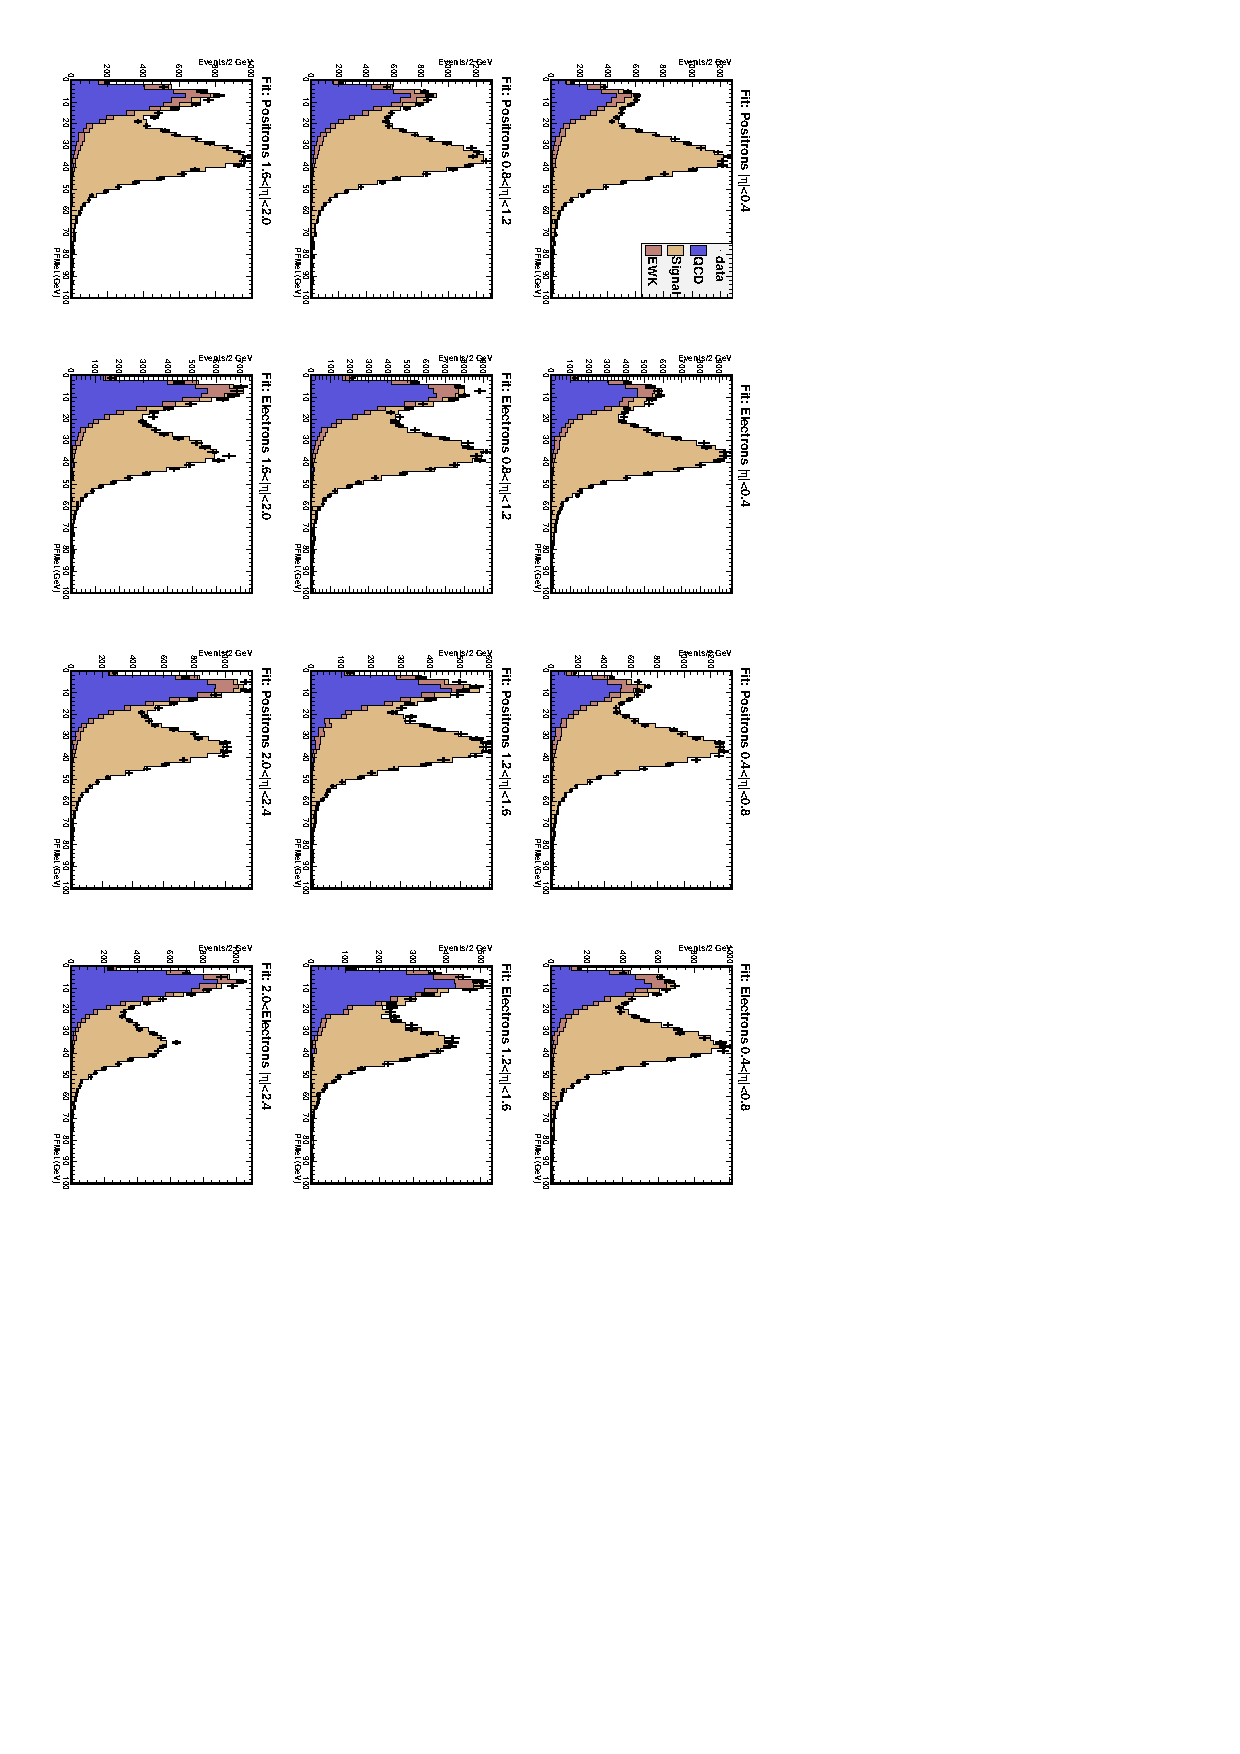
\includegraphics[angle=90,width=0.95\textwidth]{Dec22_data}
 \caption{  \label{fig:data} The fit to \ETm\ for each eta/charge bin.}
  \end{center}
\end{figure}

\begin{figure}
  \begin{center}
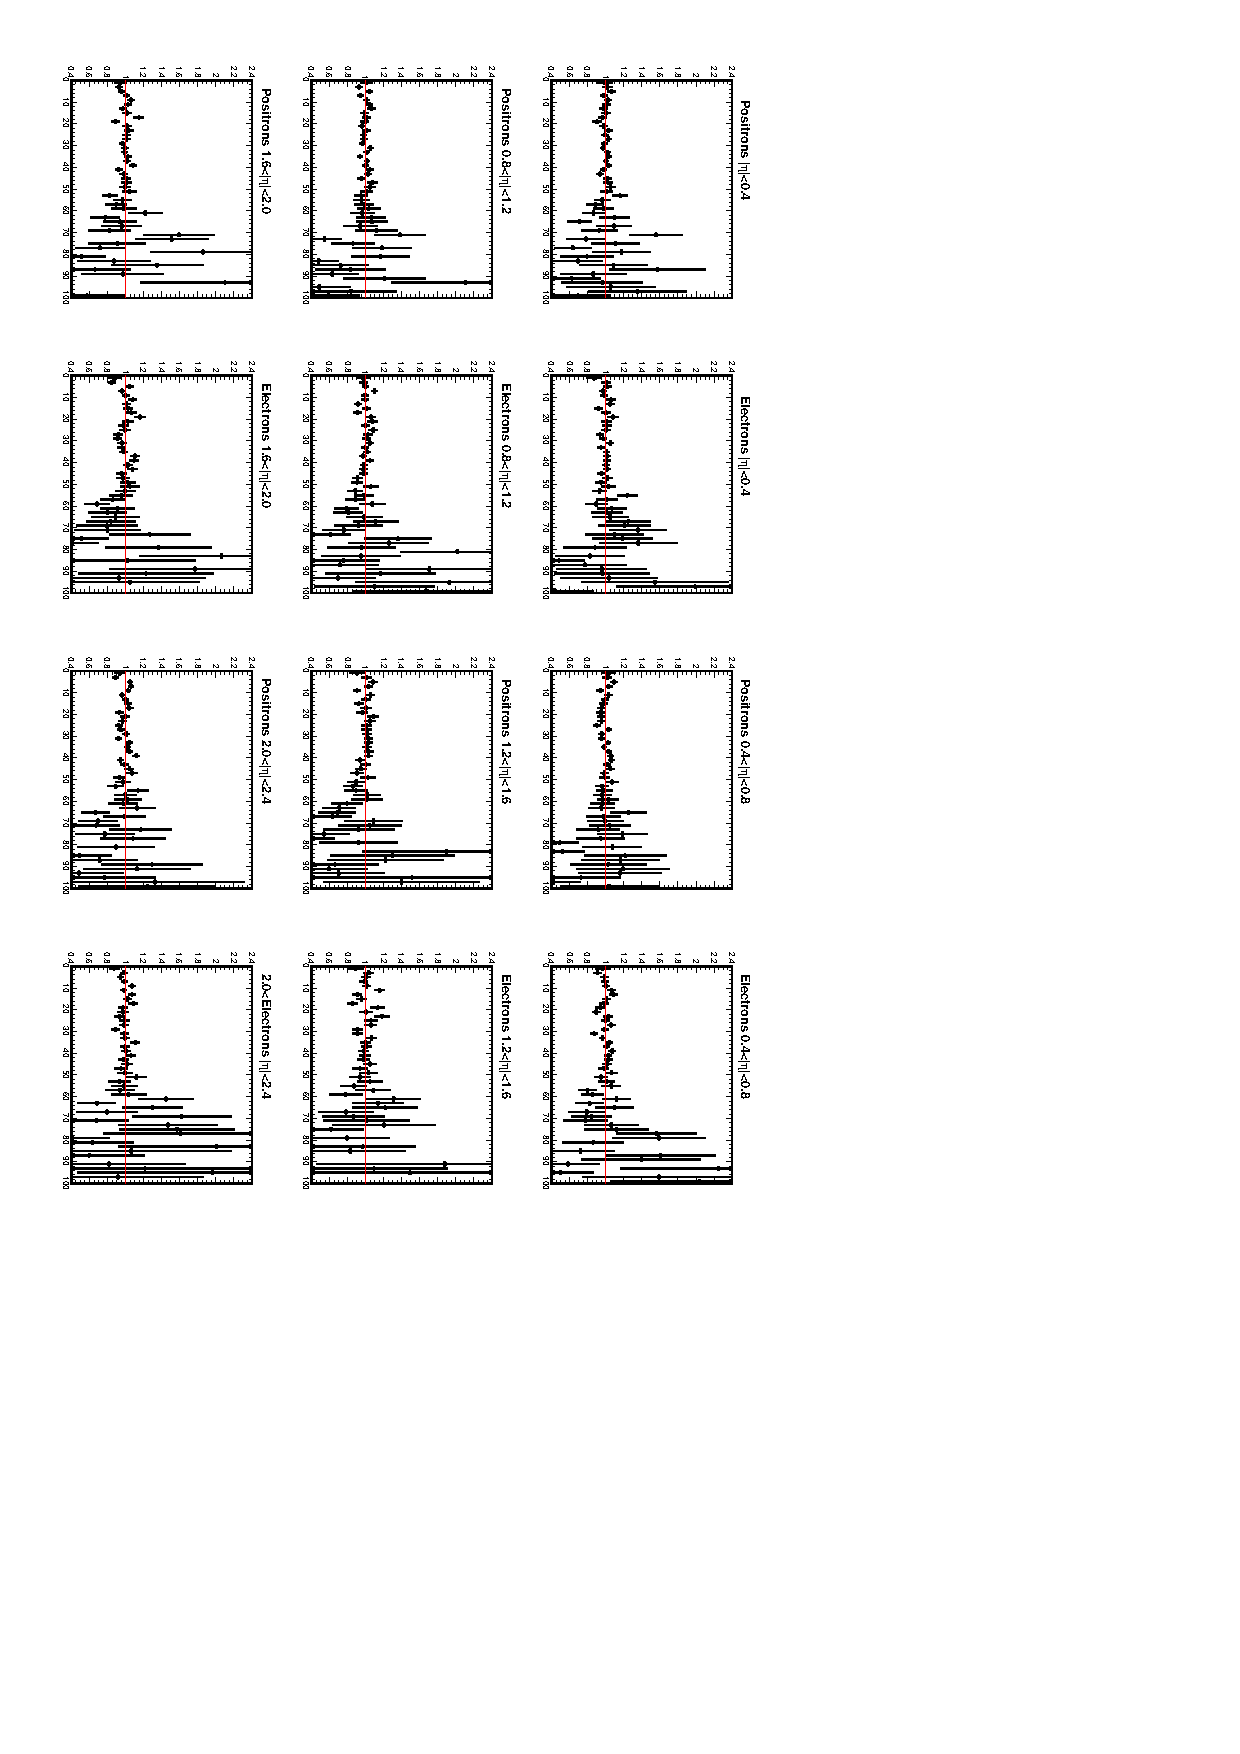
\includegraphics[angle=90,width=0.95\textwidth]{Dec22_fitratio}%width=0.9\textwidth,
     \caption{\label{fig:datafitratio}Ratio between fit and data for each eta/charge bin.}
  \end{center}
\end{figure}

\begin{table}[htb]
\begin{center}
\begin{tabular}{|lc|r|}
$|\eta|$ range &Charge & $\chi^2$/ndof of Fit\\
\hline
$0.0<| \eta |<0.4$ &+&  0.86\\
                   &-&  0.84\\
$0.4<| \eta |<0.8$ &+&  0.99\\
                   &-&  1.36\\
$0.8<| \eta |<1.2$ &+&  1.05\\
                   &-&  1.13\\
$1.2<| \eta |<1.4$ &+&  0.97\\
                   &-&  1.30\\
$1.6<| \eta |<2.0$ &+&  1.38\\
                   &-&  1.61\\
$2.0<| \eta |<2.4$ &+&  1.44\\
                   &-&  1.11\\
\end{tabular}
\caption{\label{tab:chi2}$\chi^2$/ndof of Fit.}
\end{center}
\end{table}

\section{Systematic Uncertainties}
\subsection{Relative Efficiency}

If the reconstruction efficiency of electrons is different to that of positrons
then the measured asymmetry wil be diluted and will need to be corrected for
the relative efficiency.

\begin{equation}
A_{exp}(\eta) = \frac{
                    \frac{dN}{d\eta}(e^+)-
                    \frac{\epsilon^+}{\epsilon^-}\frac{dN}{d\eta}(e^-)
                }
                {
                    \frac{dN}{d\eta}(e^+)+
                    \frac{\epsilon^+}{\epsilon^-}\frac{dN}{d\eta}(e^-)
                }
\end{equation}

The efficiency for electrons and positrons is measured using the tag and probe
method \todo{reference the CMS tag and probe method paper/note}
with a sample of \Zee events from the same datasets used in the analysis. 
The \Zee events offer a high purity source of unbiased electrons with which to
measure the efficiencies.

From the sample of \Zee events a ``tag'' electron is selected with a strict
selection criteria. 
A ``probe'' electron is selected with the same electron selection decribed
earlier.
The invariant mass of the tag-probe pair is required to be
$\unit{60}{\GeV} < M_ee < \unit{120}{\GeV}$ to ensure a high purity sample.

Efficiencies can then be calculated by measuring the signal yield in events
with one tag electron and one probe passing the selection (tag \& pass) and
events where the probe electron fails the selection (tag \& fail).
The signal yield is extracted using an simultaneous maximum likelihood fit to
both the tag \& pass and the tag \& fail samples.

For this analysis the efficiencies are measured in two parts:

\begin{itemize}
    \item GSF tracking efficiency
    \item Identification efficiency, including conversion rejection, unaminous
charge assignment and HLT request.
\end{itemize}

\begin{table}[htbp]
\begin{center}
\begin{tabular}{cccccccc}
$|\eta|$  & \multicolumn{3}{c}{GSF tracking } & \multicolumn{3}{c}{ID } & $R_\epsilon$ \\
region    & $\epsilon_{GSF}^+$ (\%) &$\epsilon_{GSF}^-$ (\%) & $R_{\epsilon_{GSF}}$ 
                                              & $\epsilon_{ID}^+$ (\%) &$\epsilon_{ID}^-$ (\%) & $R_{\epsilon_{ID}}$ &  \\
\hline
$\left[ 0.0,0.4 \right]$ & 95.7$\pm$1.1 & 97.5$\pm$1.0 & 0.982$\pm$0.015 & 71.2$\pm$1.5 & 68.4$\pm$1.5 & 1.04$\pm$0.03 &1.02$\pm$0.035  \\
$\left[ 0.4,0.8 \right]$ & 98.8$\pm$ 1.0& 98.5$\pm$1.1 & 1.003$\pm$0.015 & 72.5$\pm$1.7 & 75.6$\pm$1.6 & 0.96$\pm$0.04 &0.96$\pm$ 0.04 \\
$\left[ 0.8,1.2 \right]$ & 97.6$\pm$ 1.0& 98.4$\pm$1.0 & 0.992$\pm$0.015 & 77.4$\pm$1.5 & 74.4$\pm$1.7 & 1.04$\pm$0.04 &1.03$\pm$ 0.04 \\
$\left[ 1.2,1.4 \right]$ & 96.2$\pm$ 1.5& 96.3$\pm$1.5 & 0.999$\pm$0.022 & 69.3$\pm$2.7 & 73.0$\pm$2.6 & 0.95$\pm$0.05 &0.95$\pm$0.05  \\
$\left[ 1.6,2.0 \right]$ & 96.8$\pm$ 1.2& 96.9$\pm$1.0 & 0.999$\pm$0.015 & 61.9$\pm$2.0 & 63.6$\pm$2.0 & 0.97$\pm$0.05 &0.97$\pm$0.05  \\
$\left[ 2.0,2.4 \right]$ & 96.4$\pm$ 1.1& 97.0$\pm$1.0 & 0.994$\pm$0.015 & 58.2$\pm$2.1 & 56.7$\pm$2.1 & 1.03$\pm$0.05 &1.02$\pm$0.05  \\
\hline
$\left[ 0.0,1.4 \right]$ & 98.8$\pm$0.5 & 98.4 $\pm$0.5 & 1.004$\pm$0.007 & 84.1$\pm$0.8 & 83.8$\pm$0.8 & 1.003$\pm$0.014 & 1.007$\pm$ 0.015 \\
$\left[ 1.6,2.4 \right]$ & 98.3$\pm$0.7 & 97.8 $\pm$0.7 & 1.005$\pm$0.010 & 70.7$\pm$1.4 & 71.5$\pm$1.4 & 0.99$\pm$0.03 &0.99$\pm$ 0.03 \\
\hline 
$\left[ 0.0,2.4 \right]$ & 98.5$\pm$0.4 & 97.8$\pm$0.4 & 1.007$\pm$0.006 & 80.3$\pm$0.7 & 80.3$\pm$0.7 & 1.000$\pm$0.012 &1.007$\pm$0.014  \\
\end{tabular}
\end{center}
\caption{ GSF tracking and identification efficiency as a function of charge.}
\label{asym36:tagprobe}
\end{table}

The \TableRef{asym36:tagprobe} shows the GSF tracking effiency and identifcation 
effiency as a function of the charge.

The relative efficiency: 

\begin{equation}
R_\epsilon  =  \frac{\epsilon^+}{\epsilon^-}
\end{equation}

is found to be statistically compatible with 1 so the measured asymmetry is not
corrected for this effect.

The main systematic errors on the efficiency measurements are the energy scale
and the signal shape used to extract the signal yield. Fortunately, these
errors will cancel in the calculation of the ratio $R_\epsilon$, the difference
on  $R_\epsilon$ introduced by the energy scale and signal shape is negligable
when compared to the statistical uncertainty of the measurement, so only the
statistical uncertainty is propogated to the error in the ratio,
$dR_\epsilon$.

\begin{equation}
  \label{eq:releff}
  \sigma_{\mathcal{A}} =\mathcal{}(R_\epsilon=1) - \mathcal{A}(R_\epsilon=1\pm dR_\epsilon)  \simeq \frac{dR_\epsilon}{2}(1-\mathcal{A}^2)\simeq \frac{dR_\epsilon}{2}
\end{equation}


\subsection{Signal Extraction Method}

The systematic uncertainty due to the siganl extraction method is evaluated be
considering the error introduced be each \ETm tempalte shape used in the fit
separately.

\subsubsection{Background \ETm Shape}

\begin{figure}[htb]
 \begin{center}
 \includegraphics*[width=0.45\textwidth, angle=90]{QCDBias}
 \includegraphics*[width=0.45\textwidth, angle=90]{QCDBias_data.pdf}
 \caption{Variation on the bias on MC asymmetry measurement, using different antiselections on MC (left) and Variation on measured asymmetry on data (right).}
    \label{fig:systQCDMC}
  \end{center}
\end{figure}


The \ac{QCD} and \gjet \ETm template shape is obtained from a control sample of
events by antiselecting electrons. This may introduce a systematic bias to the
measurement if there is a difference between the anti-selected \ac{QCD} and \gjet
\ETm samples and the selected \ac{QCD} and \gjet samples.

The systematic uncertainty due to the \ac{QCD} and \gjet \ETm shape is evaluated by
varying the anti-selection used to obtain the control sample and observing the
effect that this has on the measured asymmetry.

For each variation on the antiselection, 500 pseudo-data experiments are
generated with the number of events that are expected in \unit{36.1}{\invpb} of
data. The distribution of the measured asymmetry is then fitted with a
gaussian.
The effect that changing the anti-selection has on the mean of the guassian is
studied, the maximum distance from the asymmetry measured with the nominal
anti-selection is taken as an estimate of the systematic uncertainty.

\begin{table}[htb]
\begin{center}
\begin{tabular}{crr}
$|\eta|$  &\multicolumn{2}{c}{ $\sigma(\mathcal{A}) \times 10^{-4}$}\\
   range      & MC & Data\\
\hline
$0.0<|\eta|<0.4$ & 8 & 12\\
$0.4<|\eta|<0.8$ & 7 & 9\\
$0.8<|\eta|<1.2$ & 8 & 21\\
$1.2<|\eta|<1.4$ & 12& 25\\
$1.6<|\eta|<2.0$ & 6 & 10\\
$2.0<|\eta|<2.4$ & 22& 13\\
\end{tabular}
\caption{Maximum distance between the asymmetry measured with many different antiselections
and the asymmetry measured with the chosen antiselection in MC pseudo data and real data for each eta bin.}
\label{tab:systQCD}
\end{center}
\end{table}


\subsubsection{Signal \ETm Shape from Boson Recoil}

The signam \ETm shape is constructed using information from the boson recoil.
There are three main sources of uncertainty due to the signal template,

\begin{itemize}
    \item the uncertainty in the recoil corrections,
    \item the effect the energy scale has on the recoil corrections,
    \item the uncertainty on the \ac{PDF} used to generate the events that the
recoil corrections are applied to.
\end{itemize}

To evaluate the effect of the uncertainties of the recoil method, the upper and
lower limits on the corrections are used to generate different tempaltes, and
the effect on the measured asymmetry is evaluated as a measure of the
systematic uncertainty.

The recoil method uses generator level \ac{MC} simulation as an input to the
template shape. To evaluate the efect of the generator used, templates are
generated with the CTEQ 6.6 \todo{cite the CTEQ guys here}
uncertainty \acp{PDF} which contain the central \ac{PDF} and 44 error \acp{PDF}
which contain the \unit{95}{\%} \ac{CL} for each of the 22 free parameters in
the \ac{PDF}. The maximum change in distance with respect to the central value
is taken as a measure of the systematic uncertainty.

The systematic uncertainty introduced by the electron energy scale.
\todo[inline]{electron energy scale uncertainty in the met shape}



\begin{table}[htb]
\begin{center}
\begin{tabular}{crrrr}
$|\eta|$   & \multicolumn{4}{c}{$\sigma(\mathcal{A}) \times 10^{-4}$}\\
range      & Recoil Corr. & Energy Scale & PDF & Combined \\
\hline
$0.0<|\eta|<0.4$ &  4 & 2 & 10  & 11 \\
$0.4<|\eta|<0.8$ &  6 & 3 & 15  & 16 \\
$0.8<|\eta|<1.2$ &  5 & 2 & 15  & 16 \\
$1.2<|\eta|<1.4$ &  9 & 5 & 20  & 22 \\
$1.6<|\eta|<2.0$ & 11 & 4 & 20  & 23 \\
$2.0<|\eta|<2.4$ &  7 & 3 & 20  & 21 \\
\end{tabular}
\caption{\label{tab:systSIG}Systematic uncertainty due to the Signal \ETm shape used in the signal
extraction method assigned to each eta bin.}
\end{center}
\end{table}

\subsubsection{\ac{EWK} \ETm Shape}

The \ac{EWK} shape is also generated from \ac{MC} samples. During the fitting
procedure, the \ac{EWK} shape is fixed to the \Wenu signal shape according to
the cross section taken from the \ac{MC} samples. To estimate the effect of the
uncertainty of the cross section has on the asymmetry measurement, the \ac{EWK}
background is artificially varied by \unit{$\pm20$}{ \% } and the effect on the
asymmetry is measured. Even with an over estimation of the uncertainty on the
cross section, the effect on the asymmetry is found to be small.
\begin{figure}[htb]
 \begin{center}
  \includegraphics*[width=0.6\textwidth,angle=90]{EWKFrac}
 \caption{\label{fig:systEWK}Systematic effect on asymmetry measurement by changing the electroweak background fraction by $\pm 10\%$ and $\pm 20\%$.}
  \end{center}
\end{figure}



\begin{table}[htb]
\begin{center}
\begin{tabular}{cr}
$|\eta|$ range & $\sigma(\mathcal{A}) \times 10^{-4}$\\
\hline
$0.0<|\eta|<0.4$ & 0\\
$0.4<|\eta|<0.8$ & 3\\
$0.8<|\eta|<1.2$ & 1\\
$1.2<|\eta|<1.4$ & 1\\
$1.6<|\eta|<2.0$ & 0\\
$2.0<|\eta|<2.4$ & 3\\
\end{tabular}
\caption{\label{tab:systEWK}Systematic uncertainty due to the electroweak \ETm shape used in the signal extraction method assigned to each eta bin.}
\end{center}
\end{table}


\subsection{Charge Misassignment}

The charge misassignment rate, $\omega$, is the rate at which electrons are
misasigned as positive charge and identified as positrons, and vice versa. The
misassignment induces a dilution factor to the asymmetry as a function of the
electron pseudorapidity. If it is assumed that the misassignment rate of
electrons to positrons is the same as the rate of positrons to electrons, \ie 

\begin{equation}
  \omega( \HepProcess{\APelectron \to \Pelectron} ) =
  \omega( \HepProcess{\Pelectron \to \APelectron} )
\end{equation}

then the dilution factor is given by $(1-2\omega_\eta)$ and the measured
asymmetry must be corrected by the following relation

\begin{equation}
  A_{exp}(\eta) = (1-2\omega_\eta)
                \frac{
                    \frac{dN}{d\eta}(e^+)-
                    \frac{\epsilon^+}{\epsilon^-}\frac{dN}{d\eta}(e^-)
                }
                {
                    \frac{dN}{d\eta}(e^+)+
                    \frac{\epsilon^+}{\epsilon^-}\frac{dN}{d\eta}(e^-)
                }
\end{equation}

The rate of charge misassignment is obtained from \Zee samples selected with
the same selection used in the analysis. The rate is measured by comparing the
same sign \PZ\ yield (\HepProcess{\PZ\to\Pepm\Pepm}) to the opposite sign \PZ\
yield (\HepProcess{\PZ\to\Pepm\Pemp}).





\begin{table}[htb]
  \begin{center}
\begin{tabular}{lrrrrr}
$\eta$ range        & $\omega \times 10^{-4}$  & \multicolumn{4}{c}{$\sigma(\mathcal{A})_{misch}\times 10^{-4}$} \\
                    &  & \PT $>$ 25 \GeV &  \PT $>$ 30\GeV &  \PT $>$ 35 & \PT $>$ 25 \GeV\\
      & & & & & \ETm $>$ 20 \GeV \\ \hline
$0.0<| \eta |<0.4$  & $0^{+8}$          &  2 &  2 & 2 &  2 \\ 
$0.4<| \eta |<0.8$  & $8^{+8}_{-8}$     &  3 &  2 & 2 &  3 \\
$0.8<| \eta |<1.2$  & $11^{+10}_{-8}$   &  3 &  3 & 3 &  3 \\
$1.2<| \eta |<1.4$  & $34^{+21}_{-15}$  &  8 &  7 & 6 &  7 \\
$1.6<| \eta |<2.0$  & $41^{+20}_{-15}$  &  9 &  8 & 7 &  9 \\
$2.0<| \eta |<2.4$  & $25^{+21}_{-15}$  & 10 & 10 & 9 & 11 \\
\end{tabular}
\caption{\label{tab:mischarge}Charge mismeasurement rate and systematic effect on the charge asymmetry.}
\end{center}
\end{table}


\subsection{Lepton Energy Scale and Resolution}

The energy resolution and scale of the electrons can introduce a systematic
error on the asymmetry due to the effect of of the transverse momentum cut
applied to the electrons. The largest source of electron scale bias is the
radiation induced change to the ECAL crystal transparency.

To correct fot this effect, energy scale and resolution corrrections are
derrived using a \Zee mass distribution. The corrections are parameterised by
six energy scale factors, $s_i$, and six resolutions, $\sigma_i$, one for each
pseudorapidity bin in the asymmetry measurement.
The scale factors represent the average factor each electrons \Pt in data
should be corrected to match the expected \ac{MC} energy scale.
The resolution factors represent the difference of the resolution in data and
\ac{MC}. It is the additional smearing that would need to be applied to
reconstruction level \ac{MC} to match the observed resolution in data.

A sample of \Zee events is  split in to 21 categories which correspond to all
combinations of pseudorapidity bins of the two electrons ($6+\binom{6}{2} = 21$).

A mass template s obtained in each category from \ac{MC} simulation where a
perfect \ac{ECAL} calibration is considered.

A simultaneous fit to the \Zee mass is performed in each of the 21 categories
to determine the six energy scale factors, $s_i$, and the six resolutions, 
$\sigma_i$.

In each category ($category_{ij}$) where one electron is in the $i^{th}$
pseudorapidity bin and the other is in the $j^{th}$ bin, the \ac{MC} template
mass shape is scaled by 

\begin{equation}
    \frac{1}{\sqrt{s_i s_j} } 
\end{equation}

and smeared by an addtional gaussian with width of 

\begin{equation}
    \sqrt{\sigma_i^2+\sigma_j^2}
\end{equation}

%TODO figures
\todo[inline]{Add figures to demonstrate this}

The corrections are applied to the electron before the final \Pt cut so tjat
the measured asymmetry is corrected for the energy scale.

A conservative uncertainty of \unit{1}{\% } is assigned to the electron energy
after the scale corrections. A systematic error is then estimated by measuring
the difference of the measured charge asymmetry with and without the additional
\unit{1}{\% } scale factor.

\begin{table}[htb]
  \begin{center}
    \begin{tabular}{cccc}
$\eta$ range& $\sigma{\mathcal{A}} \times 10^{-4}$  & Additional $\sigma{E_{e^\pm}}$  & $\sigma{\mathcal{A}} \times 10^{-4}$ \\
& Perfect ECAL  & from fit  &  Realistic ECAL\\
& Calibration & (GeV) & Calibration \\
\hline
$0.0<| \eta |<0.4$  &  8  & 0.2  &  4 \\
$0.4<| \eta |<0.8$  &  7  & 0.4  &  5\\
$0.8<| \eta |<1.2$  & 17  & 0.3  & 19\\
$1.2<| \eta |<1.4$  & 41  & 1.0  & 43\\
$1.6<| \eta |<2.0$  & 31  & 0.9  & 32 \\
$2.0<| \eta |<2.4$  & 41  & 0.3  & 42\\
    \end{tabular}
    \caption{\label{tab:acc}Systematic error for detector effects in the acceptace corrections.}
  \end{center}
\end{table}

\begin{table}[htb]
  \begin{center}
    \begin{tabular}{cccc}
$\eta$ range& \PT $>$ 25 \GeV & \PT $>$ 30 \GeV & \PT $>$ 35 \GeV \\
\hline
$0.0<| \eta |<0.4$  & 4 & 5 &-3 \\
$0.4<| \eta |<0.8$  & 5 & 9 & -10\\
$0.8<| \eta |<1.2$  & 19 & 9 & 32\\
$1.2<| \eta |<1.4$  & 43 &37 & 24\\
$1.6<| \eta |<2.0$  & 32 &50 & 43\\
$2.0<| \eta |<2.4$  & 42 &52 & 27\\
\end{tabular}
\caption{\label{tab:bias}Bias values due to the electron resolution for different lepton \PT cuts.}
  \end{center}
\end{table}

\begin{table}[htb]
  \begin{center}
    \begin{tabular}{cccc}
$\eta$ range& \PT $>$ 25 \GeV & \PT $>$ 30 \GeV & \PT $>$ 35 \GeV \\
\hline
$0.0<| \eta |<0.4$  & 10 & 5 & 14\\
$0.4<| \eta |<0.8$  & 7 & 15 & 44\\
$0.8<| \eta |<1.2$  & 2 & 24 & 31\\
$1.2<| \eta |<1.4$  & 19 & 27 & 46\\
$1.6<| \eta |<2.0$  & 24 & 17 & 28\\
$2.0<| \eta |<2.4$  & 16 & 17  & 44\\
\end{tabular}
\caption{\label{tab:AddScale}Systematic error due to the additional scale factor of 1\% on the energy.}
  \end{center}
\end{table}


\subsection{Systematic Uncertainty Summary}

\begin{table}[htb]
\begin{center}
\begin{tabular}{ccccccc}
\multicolumn{7}{c}{$\sigma(\mathcal{A}) \times 10^{-4}$}\\
 & Relative   & Electron  & Signal     & Charge & \ETm & Total \\
 & Efficiency & Scale/Res & Estimation & MisID  & Scale/Res & \\
\hline 
\multicolumn{7}{|c|}{$\PT > 25$ \GeV}\\
$0.0<|\eta|<0.4$ & 70 & 11 & 16 &  2 &  0 &  73\\
$0.4<|\eta|<0.8$ & 70 &  9 & 19 &  3 &  0 &  73\\
$0.8<|\eta|<1.2$ & 70 & 19 & 26 &  3 &  0 &  77\\
$1.2<|\eta|<1.4$ & 70 & 47 & 33 &  8 &  0 &  90 \\
$1.6<|\eta|<2.0$ & 70 & 40 & 25 &  9 &  0 &  85\\
$2.0<|\eta|<2.4$ & 70 & 45 & 25 & 10 &  0 &  87\\
\hline
\multicolumn{7}{|c|}{$\PT > 30$ \GeV}\\
$0.0<|\eta|<0.4$ & 70 &  7 & 16 &  2 &  0 &  72 \\
$0.4<|\eta|<0.8$ & 70 & 17 & 19 &  2 &  0 &  75 \\
$0.8<|\eta|<1.2$ & 70 & 26 & 26 &  3 &  0 &  79 \\
$1.2<|\eta|<1.4$ & 70 & 46 & 33 &  7 &  0 &  91 \\
$1.6<|\eta|<2.0$ & 70 & 53 & 25 &  8 &  0 &  92 \\
$2.0<|\eta|<2.4$ & 70 & 55 & 25 & 10 &  0 &  93 \\
\hline 
\multicolumn{7}{|c|}{$\PT > 35$ \GeV}\\
$0.0<|\eta|<0.4$ & 70 & 14 & 16 &  2 &  0 & 73 \\
$0.4<|\eta|<0.8$ & 70 & 45 & 19 &  2 &  0 & 85 \\
$0.8<|\eta|<1.2$ & 70 & 44 & 26 &  3 &  0 & 87 \\
$1.2<|\eta|<1.4$ & 70 & 52 & 33 &  6 &  0 & 93 \\
$1.6<|\eta|<2.0$ & 70 & 51 & 25 &  7 &  0 & 94 \\
$2.0<|\eta|<2.4$ & 70 & 52 & 25 &  9 &  0 & 94 \\
\hline 
\multicolumn{7}{|c|}{$\PT > 25$ \GeV $\ETm >
$ \GeV}\\
$0.0<|\eta|<0.4$ & 70 & 11 & 16 &  2 & 16 & 74 \\
$0.4<|\eta|<0.8$ & 70 &  9 & 19 &  3 & 14 & 74 \\
$0.8<|\eta|<1.2$ & 70 & 19 & 26 &  3 & 20 & 80 \\
$1.2<|\eta|<1.4$ & 70 & 47 & 33 &  7 & 24 & 94 \\
$1.6<|\eta|<2.0$ & 70 & 40 & 25 &  9 & 15 & 86 \\
$2.0<|\eta|<2.4$ & 70 & 45 & 25 & 11 & 28 & 92 \\
\end{tabular}
\caption{\label{tab:summarysyst}Summary of the systematic errors}
\end{center}
\end{table}


% This sectionn may not be included
\section{Additional Systematic Studies}
\subsection{Cross Checks}
\subsubsection{Positive vs Negative Eta}
\subsubsection{Use of pure ECAL Energy Measurement}
\subsection{Asymmetric \ac{QCD} Background}



\section{Results}

\begin{figure}[htb]
  \begin{center}
  \includegraphics*[width=0.45\textwidth,angle=90]{Asym_25}
  \caption{\label{fig:asym25} Measured electron charge asymmetry corrected with predictions from CTEQ10W and MSTW08NNLO.}
  \end{center}
\end{figure}

\begin{table}[htb]
\begin{center}
\begin{tabular}{crrrr}
$|\eta|$ range & $<|\eta|>$ & Data & CTEQ6.6 & MSTW \\
\hline 
$0.0<|\eta|<0.4$ & 0.2 & $0.1541\pm0.0064\pm0.0073$ & $0.1502^{+0.0062}_{-0.0045}$ & $0.1296^{+0.0022}_{-0.0032}$\\
$0.4<|\eta|<0.8$ & 0.6 & $0.1666\pm0.0064\pm0.0073$ & $0.1682^{+0.0060}_{-0.0055}$ & $0.1458^{+0.0023}_{-0.0031}$\\
$0.8<|\eta|<1.2$ & 1.0 & $0.1728\pm0.0065\pm0.0077$ & $0.1944^{+0.0051}_{-0.0072}$ & $0.1737^{+0.0026}_{-0.0030}$\\
$1.2<|\eta|<1.4$ & 1.3 & $0.1895\pm0.0096\pm0.0090$ & $0.2216^{+0.0050}_{-0.0087}$ & $0.1976^{+0.0032}_{-0.0026}$\\
$1.6<|\eta|<2.0$ & 1.8 & $0.2331\pm0.0076\pm0.0085$ & $0.2672^{+0.0047}_{-0.0105}$ & $0.2454^{+0.0039}_{-0.0018}$\\
$2.0<|\eta|<2.4$ & 2.2 & $0.2670\pm0.0077\pm0.0087$ & $0.2821^{+0.0037}_{-0.0110}$ & $0.2619^{+0.0039}_{-0.0018}$\\
\end{tabular}
\caption{Measured electron charge asymmetry with predictions from CTEQ6.6 and MSTW PDFs.  36 Uncertainties on measured asymmetry are statistical and systematic respectivly and the Uncertainties on predictions are due to the uncertainties on the PDFs}
\label{tab:results}
\end{center}
\end{table}




\subsection{Results in Bins of Lepton Momentum and \ETm}

\begin{figure}[htb]
  \begin{center}
  \includegraphics*[width=0.45\textwidth,angle=90]{Asym_30}
  \caption{\label{fig:asym30}Measured electron charge asymmetry for lepton momentum $\PT>30$ with predictions from CTEQ10W and MSTW08NNLO.}
  \end{center}
\end{figure}

\begin{figure}[htb]
  \begin{center}
\includegraphics*[width=0.45\textwidth,angle=90]{Asym_35}
  \caption{\label{fig:asym35}Measured electron charge asymmetry for lepton momentum $\PT>35$ \GeV with predictions from CTEQ10W and MSTW08NNLO.}
  \end{center}
\end{figure}


\begin{table}[htb]
\begin{center}
\begin{tabular}{crrr}
$|\eta|$   & $<|\eta|>$ & \multicolumn{2}{c}{$\PT>30$ \GeV} \\
range                  &      & Data & Prediction                   \\
\hline    
$0.0<|\eta|<0.4$ & 0.2 & $0.1330\pm0.0071\pm0.0072$ & $0.1331^{+0.0058}_{-0.0026}$\\
$0.4<|\eta|<0.8$ & 0.6 & $0.1501\pm0.0071\pm0.0075$ & $0.1501^{+0.0030}_{-0.0028}$\\
$0.8<|\eta|<1.2$ & 1.0 & $0.1508\pm0.0073\pm0.0079$ & $0.1713^{+0.0035}_{-0.0034}$\\
$1.2<|\eta|<1.4$ & 1.3 & $0.1651\pm0.0106\pm0.0091$ & $0.1947^{+0.0032}_{-0.0050}$\\
$1.6<|\eta|<2.0$ & 1.8 & $0.2082\pm0.0087\pm0.0092$ & $0.2417^{+0.0058}_{-0.0063}$\\
$2.0<|\eta|<2.4$ & 2.2 & $0.2451\pm0.0086\pm0.0093$ & $0.2625^{+0.0070}_{-0.0080}$\\
\end{tabular}
\caption{Measured electron charge asymmetry in lepton momentum $\PT>30$ \GeV
with predictions from CTEQ6.6.  Uncertainties on measured asymmetry are
statistical and systematic respectivly and the Uncertainties on predictions are
due to the uncertainties on the PDF}.
\label{tab:results30}
\end{center}
\end{table}


\begin{table}[htb]
\begin{center}
\begin{tabular}{crrr}
$|\eta|$ & $<|\eta|>$ & \multicolumn{2}{c}{$\PT>35$ \GeV}    \\
range                  &     &  Data                        & Prediction    \\
\hline
$0.0<|\eta|<0.4$ & 0.2 & $0.1191\pm0.0085\pm0.0073$ & $0.1147^{+0.0025}_{-0.0023}$\\
$0.4<|\eta|<0.8$ & 0.6 & $0.1259\pm0.0084\pm0.0085$ & $0.1267^{+0.0024}_{-0.0026}$\\
$0.8<|\eta|<1.2$ & 1.0 & $0.1350\pm0.0087\pm0.0087$ & $0.1495^{+0.0034}_{-0.0036}$\\
$1.2<|\eta|<1.4$ & 1.3 & $0.1385\pm0.0128\pm0.0093$ & $0.1686^{+0.0043}_{-0.0043}$\\
$1.6<|\eta|<2.0$ & 1.8 & $0.1834\pm0.0105\pm0.0094$ & $0.2170^{+0.0057}_{-0.0069}$\\
$2.0<|\eta|<2.4$ & 2.2 & $0.2220\pm0.0105\pm0.0094$ & $0.2432^{+0.0081}_{-0.0089}$\\
\end{tabular}
\caption{Measured electron charge asymmetry in lepton momentum $\PT>35$ \GeV with predictions from CTEQ6.6.
Uncertainties on measured asymmetry are statistical and systematic respectivly and the
Uncertainties on predictions are due to the uncertainties on the PDF}
\label{tab:results35}
\end{center}
\end{table}



%\subsection{Correction for the Electron and \ETm Resolution Effect}
% think about this...



  \chapter{ 
Measurement of the electron charge asymmetry with \unit{840}{\invpb} }

The measurement detailed in the previous chapter was performed with
\unit{36}{\invpb} of data from the full 2010 dataset. 
In this next chapter, the update to the measurement of the electron charge asymmetry in
inclusive \inclusiveWe production with \unit{840}{\invpb} is presented. 
The data was collected with the \ac{CMS} detector from collisions from the
first 2011 \ac{LHC} run (Run A) and corresponds to a 25 times increase in
statistics over the 2010 measurement.


The majority of the 2011 analysis is identical to the 2010 analysis,
however small changes to the metheodolgy have been implemented due to changes
in the luminosity and the increase in data in the 2011 \ac{LHC} run.

\section{Event Selection}
\subsection{Trigger}


\begin{table}[htbp]
  \begin{center}
    \leavevmode
     \begin{tabular}{ll} 
      Run Ranges & Trigger  \\
     \hline
     160404-161176 & HLT\_Ele27\_CaloIdVT\_CaloIsoT\_TrkIdT\_TrkIsoT\_v1  \\
     161217-163261 & HLT\_Ele32\_CaloIdVT\_CaloIsoT\_TrkIdT\_TrkIsoT\_v1  \\
     163270-163869 & HLT\_Ele32\_CaloIdVT\_CaloIsoT\_TrkIdT\_TrkIsoT\_v2  \\
     165088-165633 & HLT\_Ele32\_CaloIdVT\_CaloIsoT\_TrkIdT\_TrkIsoT\_v3  \\
     165970-166967 & HLT\_Ele32\_CaloIdVT\_CaloIsoT\_TrkIdT\_TrkIsoT\_v4  \\
     \end{tabular}

  \caption{Triggers used to select the data used in this measurement.}
  \label{asym840:triggers}

   \end{center}
\end{table}


The definitions of the triggers follows the same pattern as described in 
\SectionRef{asym36:triggerdef}.

Due to the increased luminosity in the 2011 Run A, the identifaction and
isolation cuts applied to the trigger have been tightened. The \PT cut applied
to the electon have been increased, first to \unit{27}{\GeV} and then in later
runs to \unit{32}{\GeV}.

\subsection{Electron Selection}


 \begin{table}[htbp]
   \begin{center}
     \leavevmode
     \begin{tabular}{lcc} 
       \multicolumn{1}{c}{Variable} & \multicolumn{1}{c}{cut value (barrel)}& \multicolumn{1}{c}{cut value (endcap)}\\
         \hline   
 \multicolumn{3}{l}{ID Cuts}\\ 
         H/E & 0.04 & 0.025 \\
         $\Delta\phi$ & 0.06 & 0.03 \\
         $\Delta\eta$ & 0.004 & 0.007  \\
         $\sigma_{\eta\eta}$ & 0.01 & 0.03 \\ \hline
 \multicolumn{3}{l}{Isolation Cuts}\\ 
   $ISO_{trk} / E_T $  & 0.09 & 0.04 \\
   $ISO_{ecal}/ E_T$  & 0.07 & 0.05 \\
   $ISO_{hcal}/ E_T$  & 0.10 & 0.025 \\ \hline
 \multicolumn{3}{l}{Conversion Rejection Cuts}\\ \hline
   Missing Hits  & \multicolumn{2}{c}{$\leq 0$}\\
   Dist $||$ Dcot   & \multicolumn{2}{c}{$>0.02$}\\
     \end{tabular}
     \caption{Electron selection variables and corresponding cut values.}
     \label{asym840:electronselection}
   \end{center}
 \end{table}

The electron transverse momentum cut is shifted up to \unit{35}{\GeV} due to
the trigger contraints. This is the only change with respect to the 2010
analysis on the electron selection, detailed in
\TableRef{asym840:electronselection}.

\subsection{Event Selection}
The event selection remains the same with respect to the 2010 measurement.
An Event is selected if if contains a single electron that passes all electron
selection.
To removed Drell-Yan events an event is vetoed if it contains a second lepton
(an electron passing a loose selecton, or an isolated muon) with $\PT > 
\unit{15}{\GeV}$

The Particle Flow \ETm distribution for the events that pass the event
selection, with $\PT > \unit{35}{\GeV}$ and $|\eta| < 2.4$ is shown in
\FigureRef{asym840:pfmet}.

\begin{figure}[htb]
  \centering
  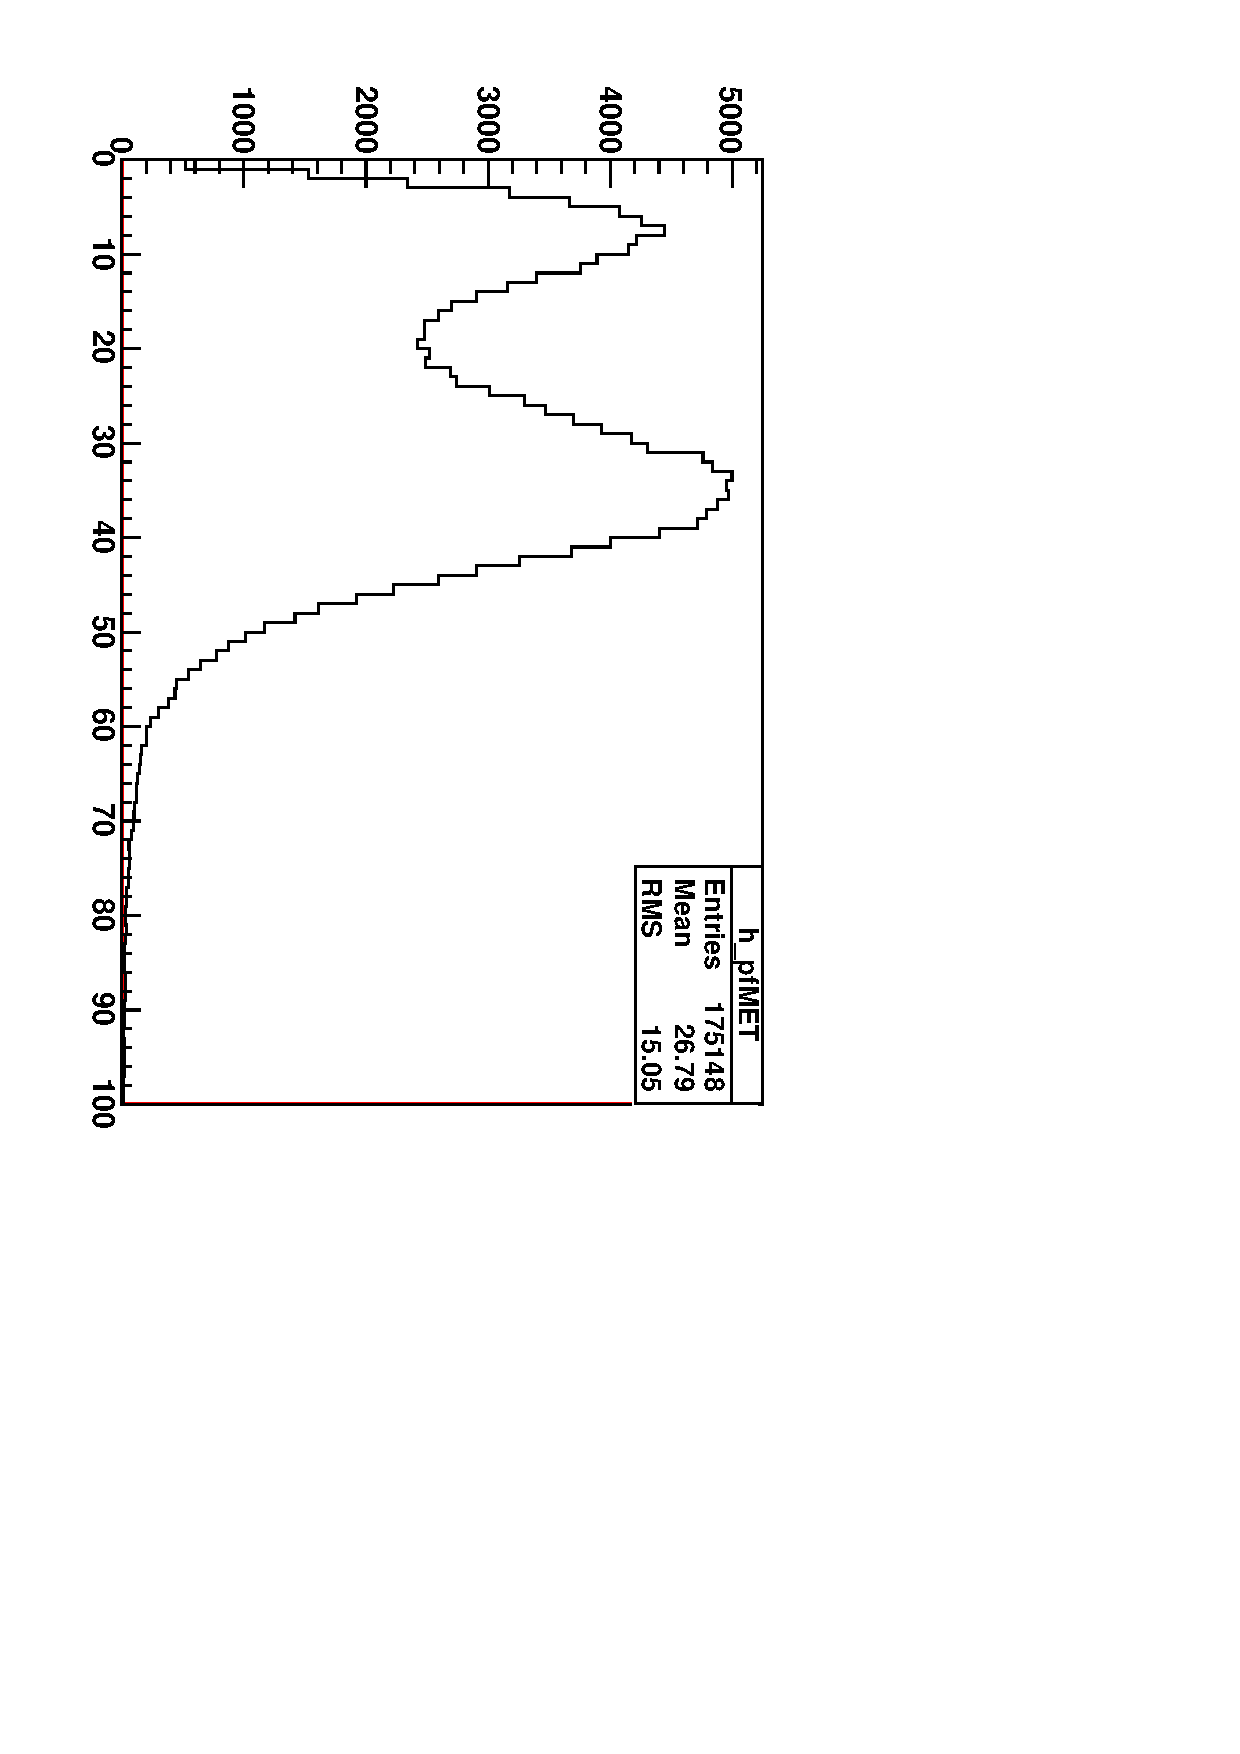
\includegraphics[width=0.5\textwidth]{pfmet}
  \caption{Particle Flow \ETm distribution for selected events.}
  \label{asym840:pfmet}
\end{figure}

The number of selected events that pass the event selection are shown in
\TableRef{asym36:selectedevents}.

\begin{table}[htb]
 \begin{center}
 \begin{tabular}{lcc}
 $|\eta|$ range & Selected Positrons & Selected Electrons\\
 \hline
 $0.0<| \eta |<0.2$ & 108235 &  90860 \\
 $0.2<| \eta |<0.4$ & 112870 &  93996 \\
 $0.4<| \eta |<0.6$ & 114148 &  94721 \\
 $0.6<| \eta |<0.8$ & 117099 &  95295 \\
 $0.8<| \eta |<1.0$ & 116956 &  94580 \\
 $1.0<| \eta |<1.2$ & 113336 &  90755 \\
 $1.2<| \eta |<1.4$ & 115265 &  91572 \\
 $1.6<| \eta |<1.8$ &  92137 &  70205 \\
 $1.8<| \eta |<2.0$ & 105596 &  80921 \\
 $2.0<| \eta |<2.2$ & 112419 &  86240 \\
 $2.2<| \eta |<2.4$ & 121224 & 102111 \\
 \end{tabular}
 \caption{Number of events passing the event selection for lepton momentum cut
 of \unit{\PT>35}{\GeV}.}
\label{asym840:selectedevents}
\end{center}
\end{table}

The exected composition of the selected events, derived from MC simulation
samples, is show in \TableRef{asym840:selectedcomp}. 

\begin{table}[htb]
\begin{center}
\begin{tabular}{lr}
& \unit{\PT>35}{\GeV}\\ \hline
$W\rightarrow e\nu$  & 76.2$\%$\\
QCD Background       & 16.0$\%$\\
EWK Total Background & 7.8$\%$ \\
~ EWK DYtautau      & 0.2$\%$  \\
~ EWK DYee          & 6.4$\%$  \\
~ EWK Wtaunu        & 0.8$\%$ \\
~ EWK ttbar         & 0.4$\%$ \\
\end{tabular}
\caption{Composition of selected events for lepton momentum cut of
  \unit{\PT>35}{\GeV}. Numbers are evaluated using simulation.}
 \label{asym840:selectedcomp}
\end{center}
\end{table}

\section{Signal Yield Extraction}
\todo[inline]{Summary of signal yield extraction method}

\subsection{QCD \ETm Shape}
\todo[inline]{background MET shape explanation. talk about antiselections in
some detail.}

\begin{table}[htbp]
  \begin{center}
    \leavevmode
    \begin{tabular}{lcc} 
      \multicolumn{1}{c}{Variable} & \multicolumn{1}{c}{cut value (barrel)}& \multicolumn{1}{c}{cut value (endcap)}\\\hline
        H/E & 0.04 & 0.025 \\
        $\Delta\phi$ & $>0.06$  & $>0.04$ \\
        $\Delta\eta$ & $>0.007$ & $>0.009$\\
  $ISO_{trk} / E_T $ & 0.09 & 0.04 \\
  $ISO_{ecal}/ E_T$  & 0.07 & 0.05 \\
  $ISO_{hcal}/ E_T$  & 0.10 & 0.025\\
    \end{tabular}
    \caption{Electron anti-selection variables and corresponding cut values. $\Delta\phi$ and $\Delta\eta$ cuts are inverted.}
    \label{asym840:AScuts}
  \end{center}
\end{table}

\subsection{Signal \ETm Shape from Boson Recoil}
\todo[inline]{Signal MET shape explanation. Quite a bit can be written here
about the boson recoil.}

\subsection{EWK \ETm Shape}
\todo[inline]{EWK MET shape explanation}


\subsection{Validation of Signal Extraction Method on Simulation}
\todo[inline]{pseudo data trials}

\subsection{Fit on Real Data}
\todo[inline]{Fit applied to data and uncorrected results.}

\begin{figure}
  \begin{center}
    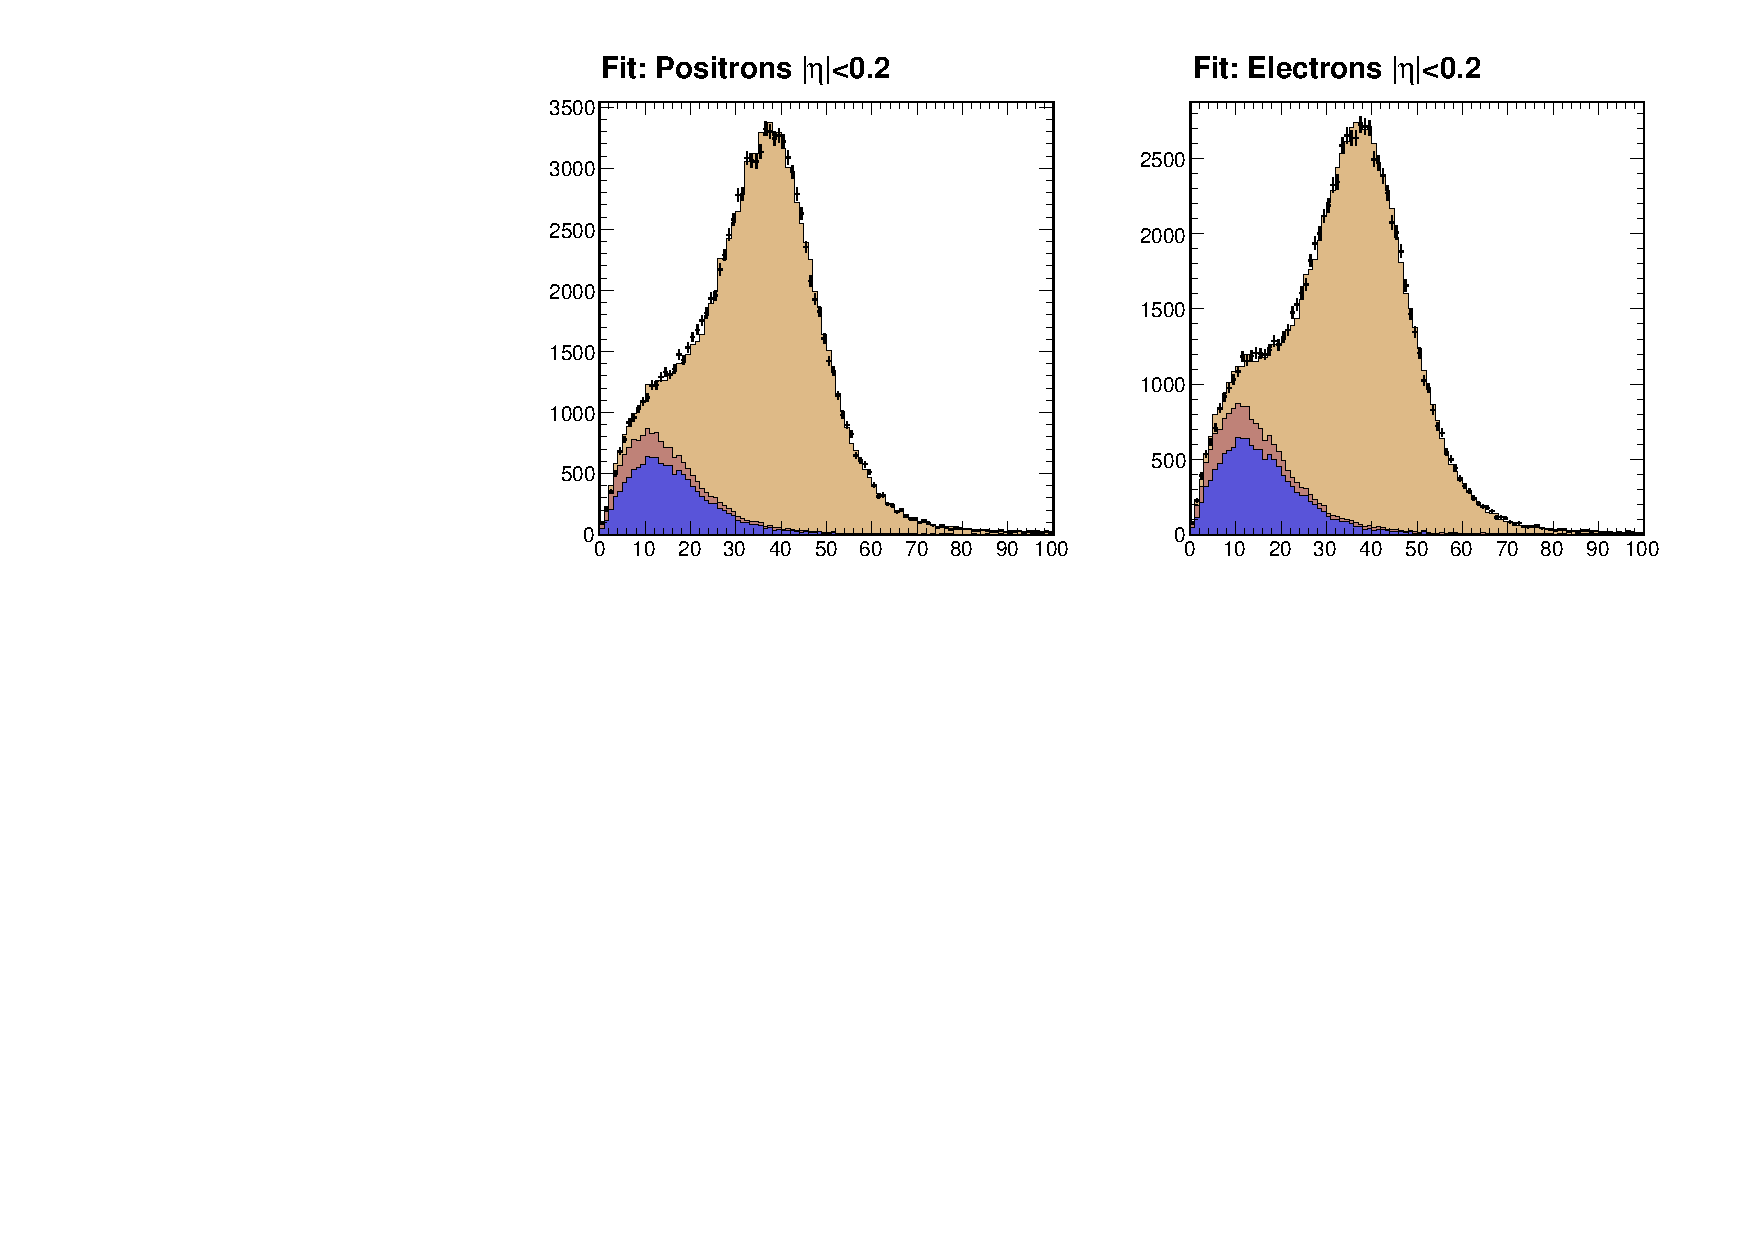
\includegraphics[width=0.95\textwidth]{data_0.pdf} \\
    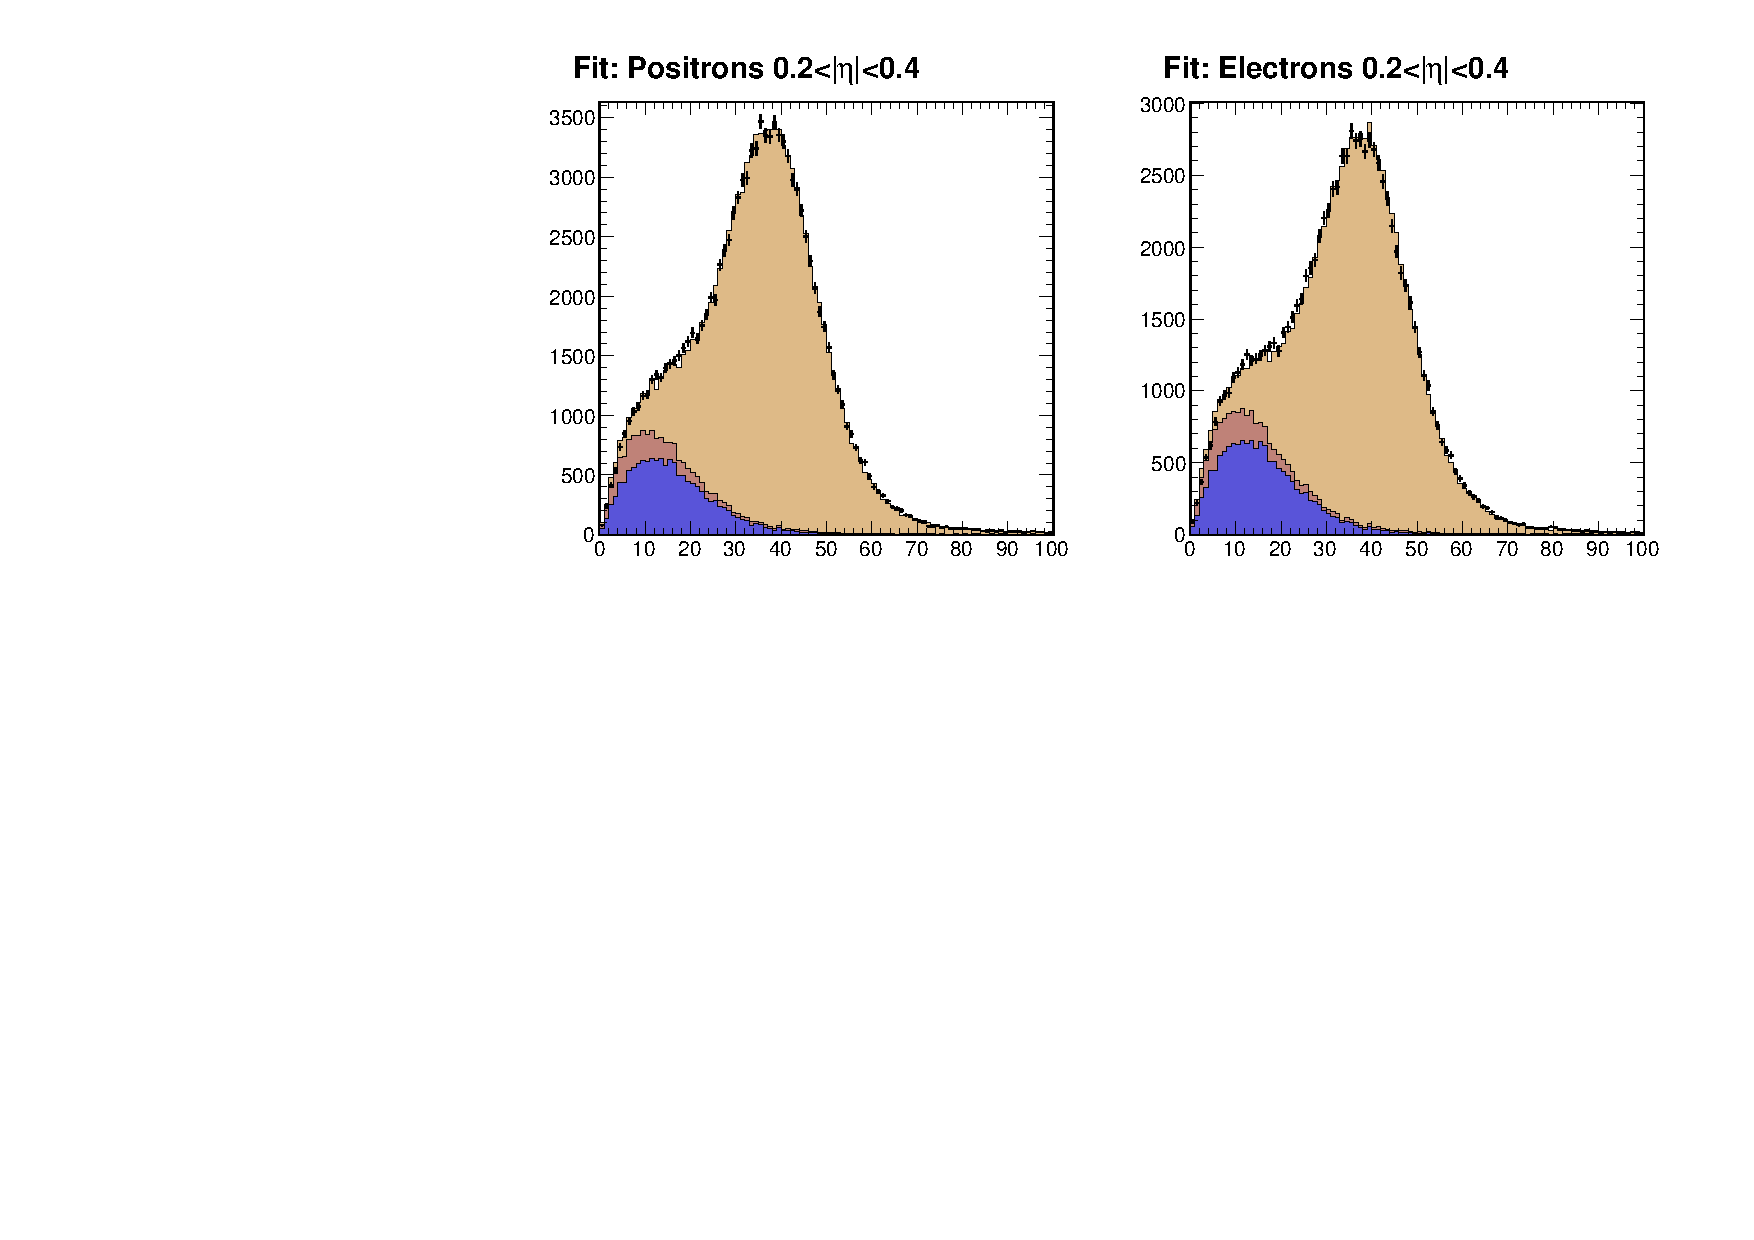
\includegraphics[width=0.95\textwidth]{data_1.pdf} \\
    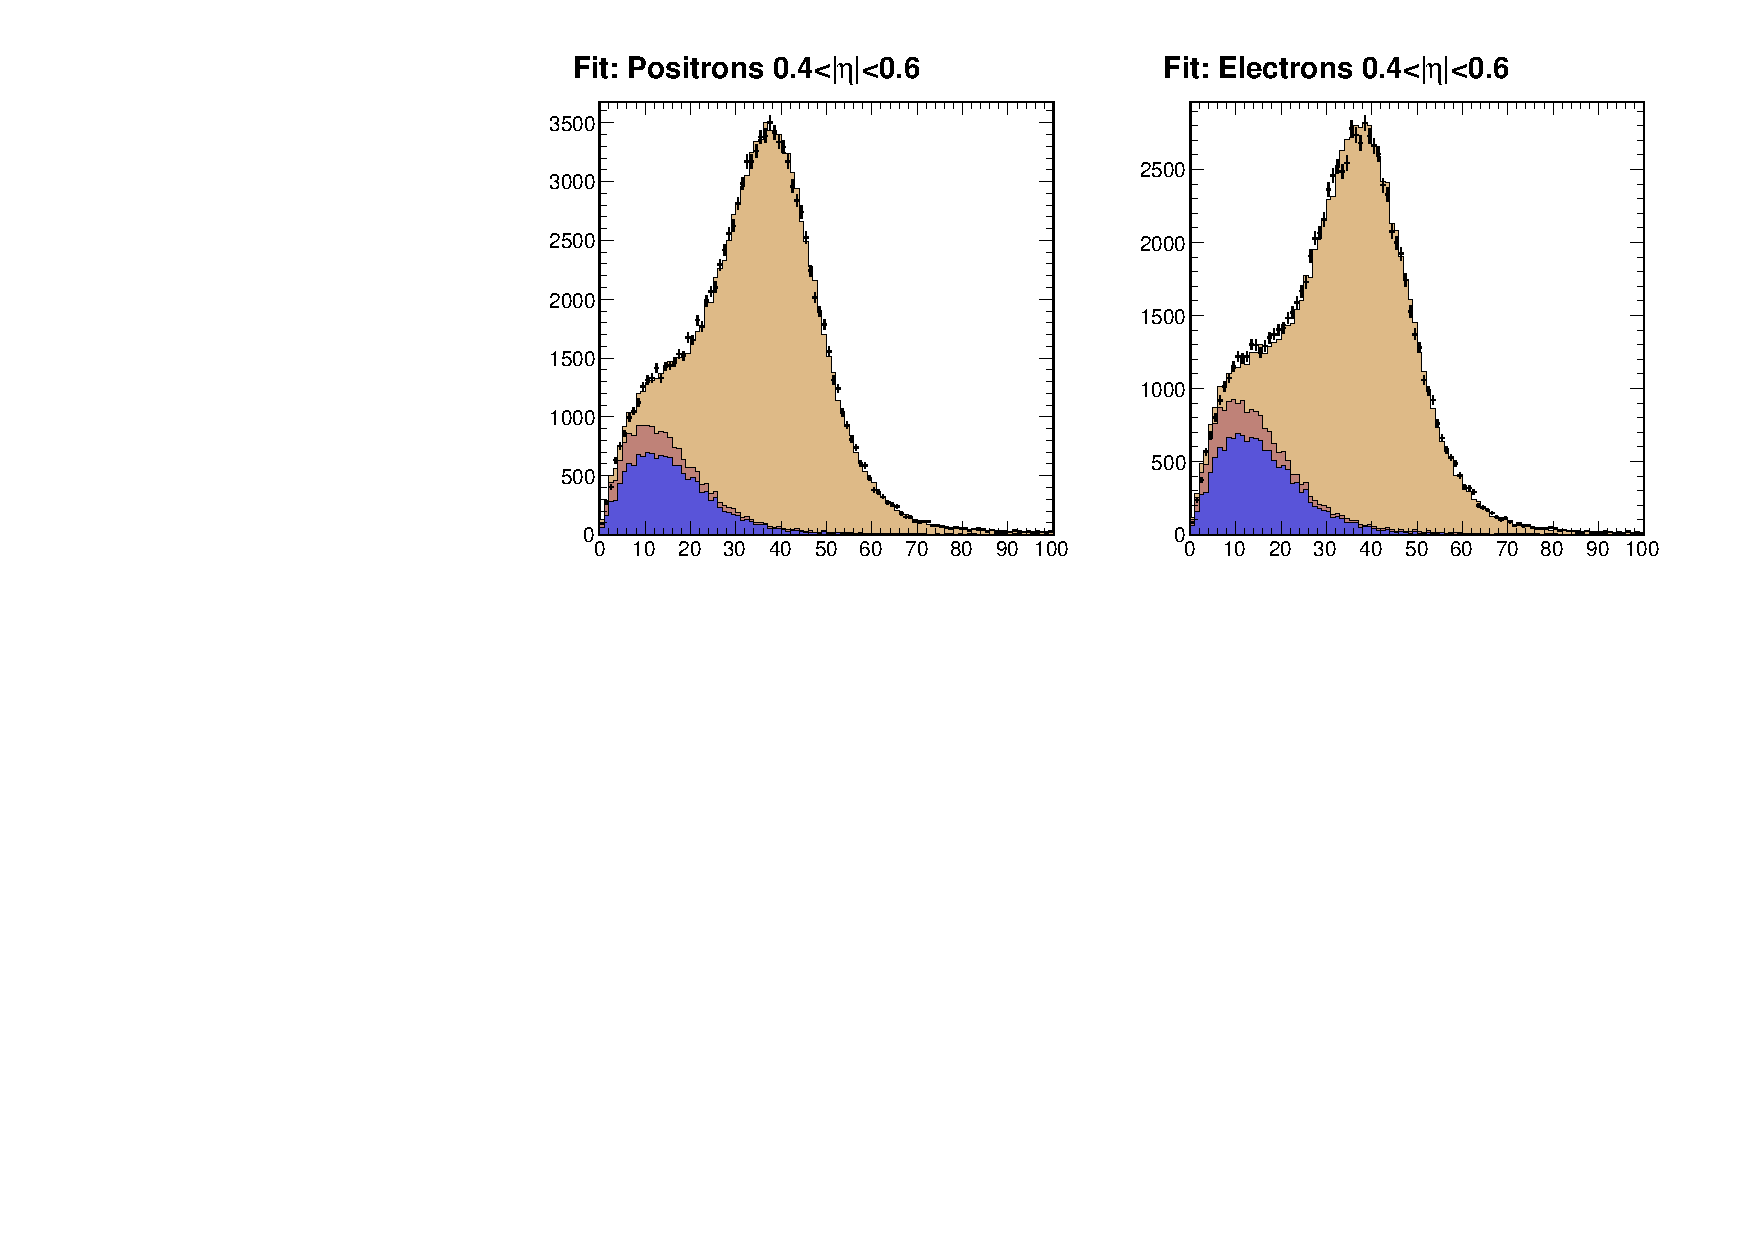
\includegraphics[width=0.95\textwidth]{data_2.pdf}
 \caption{  \label{fig:data1} The fit to \MET\ for eta bins 1,2 and 3.}
  \end{center}
\end{figure}

\begin{figure}
  \begin{center}
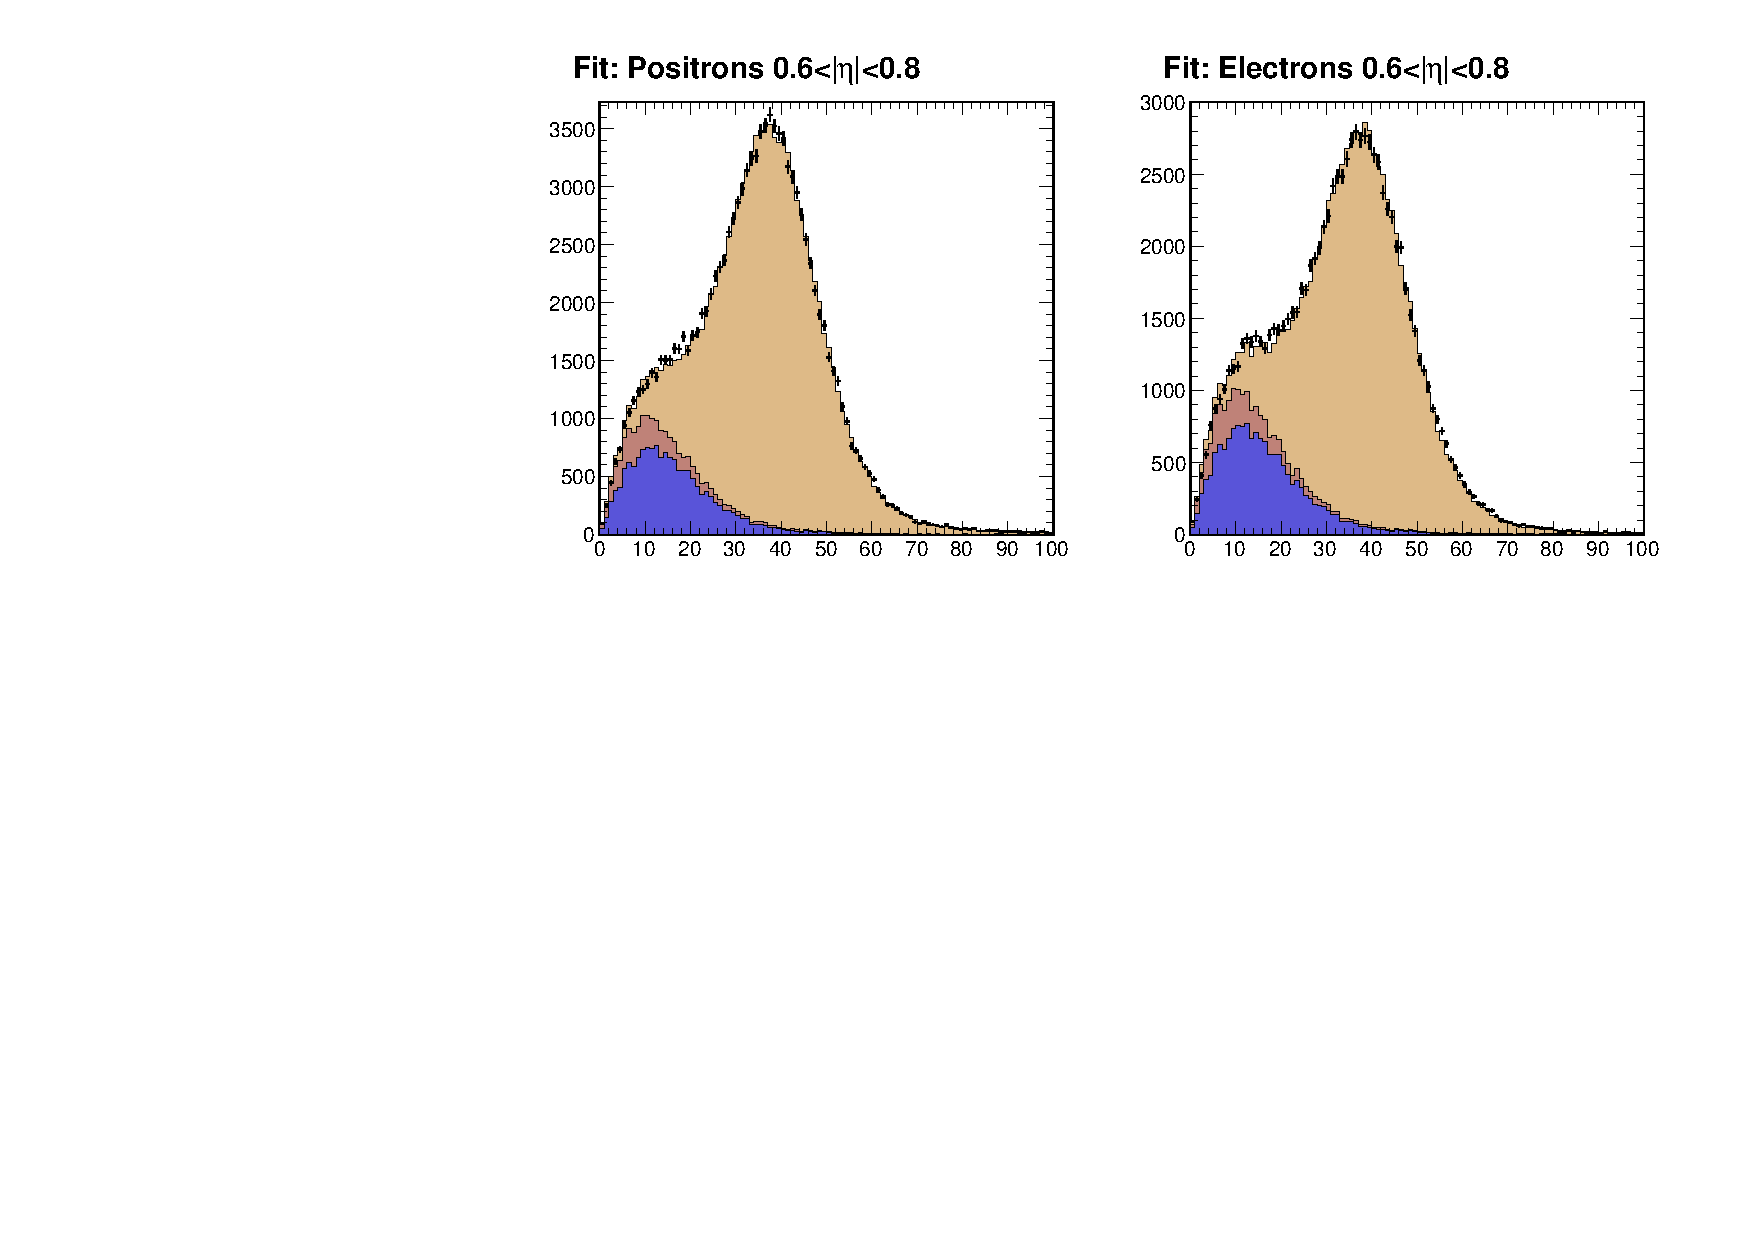
\includegraphics[width=0.95\textwidth]{data_3.pdf} \\
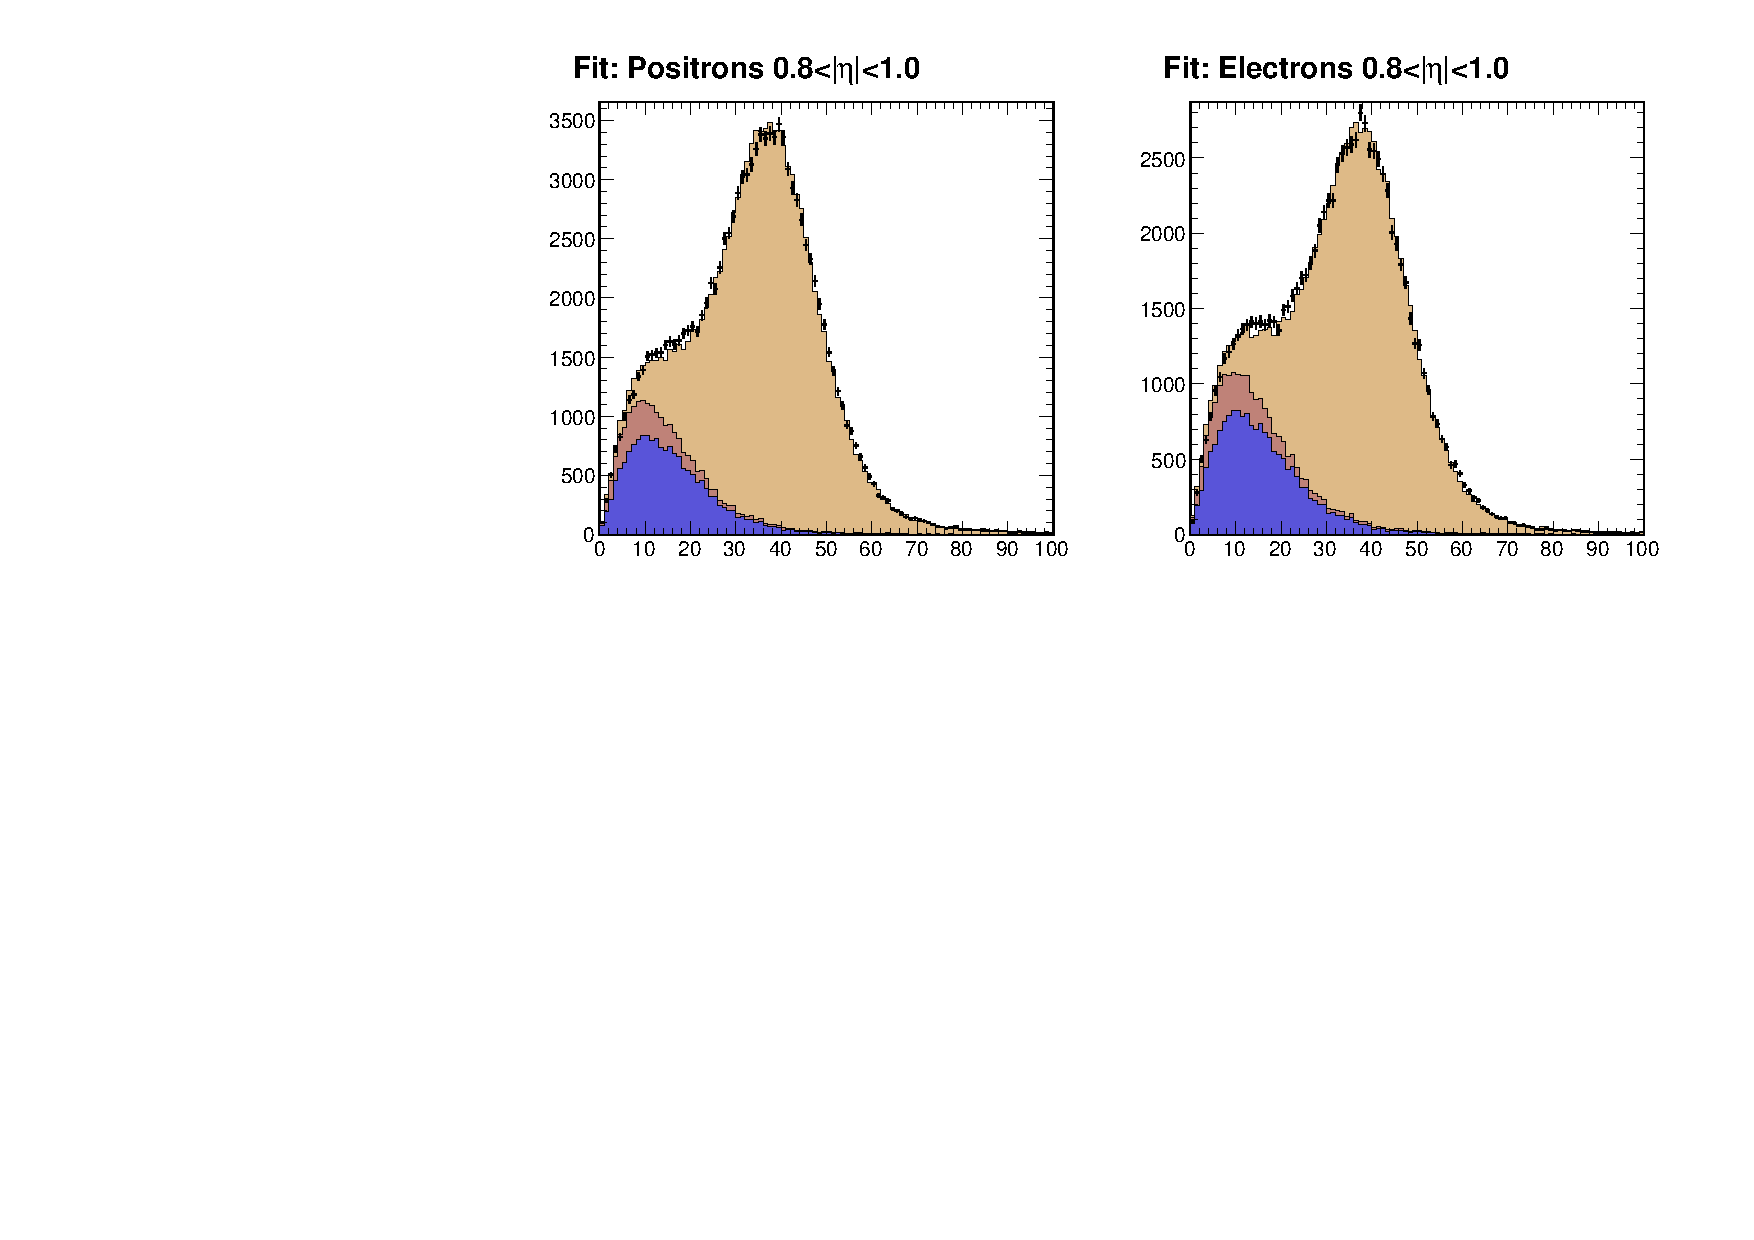
\includegraphics[width=0.95\textwidth]{data_4.pdf} \\
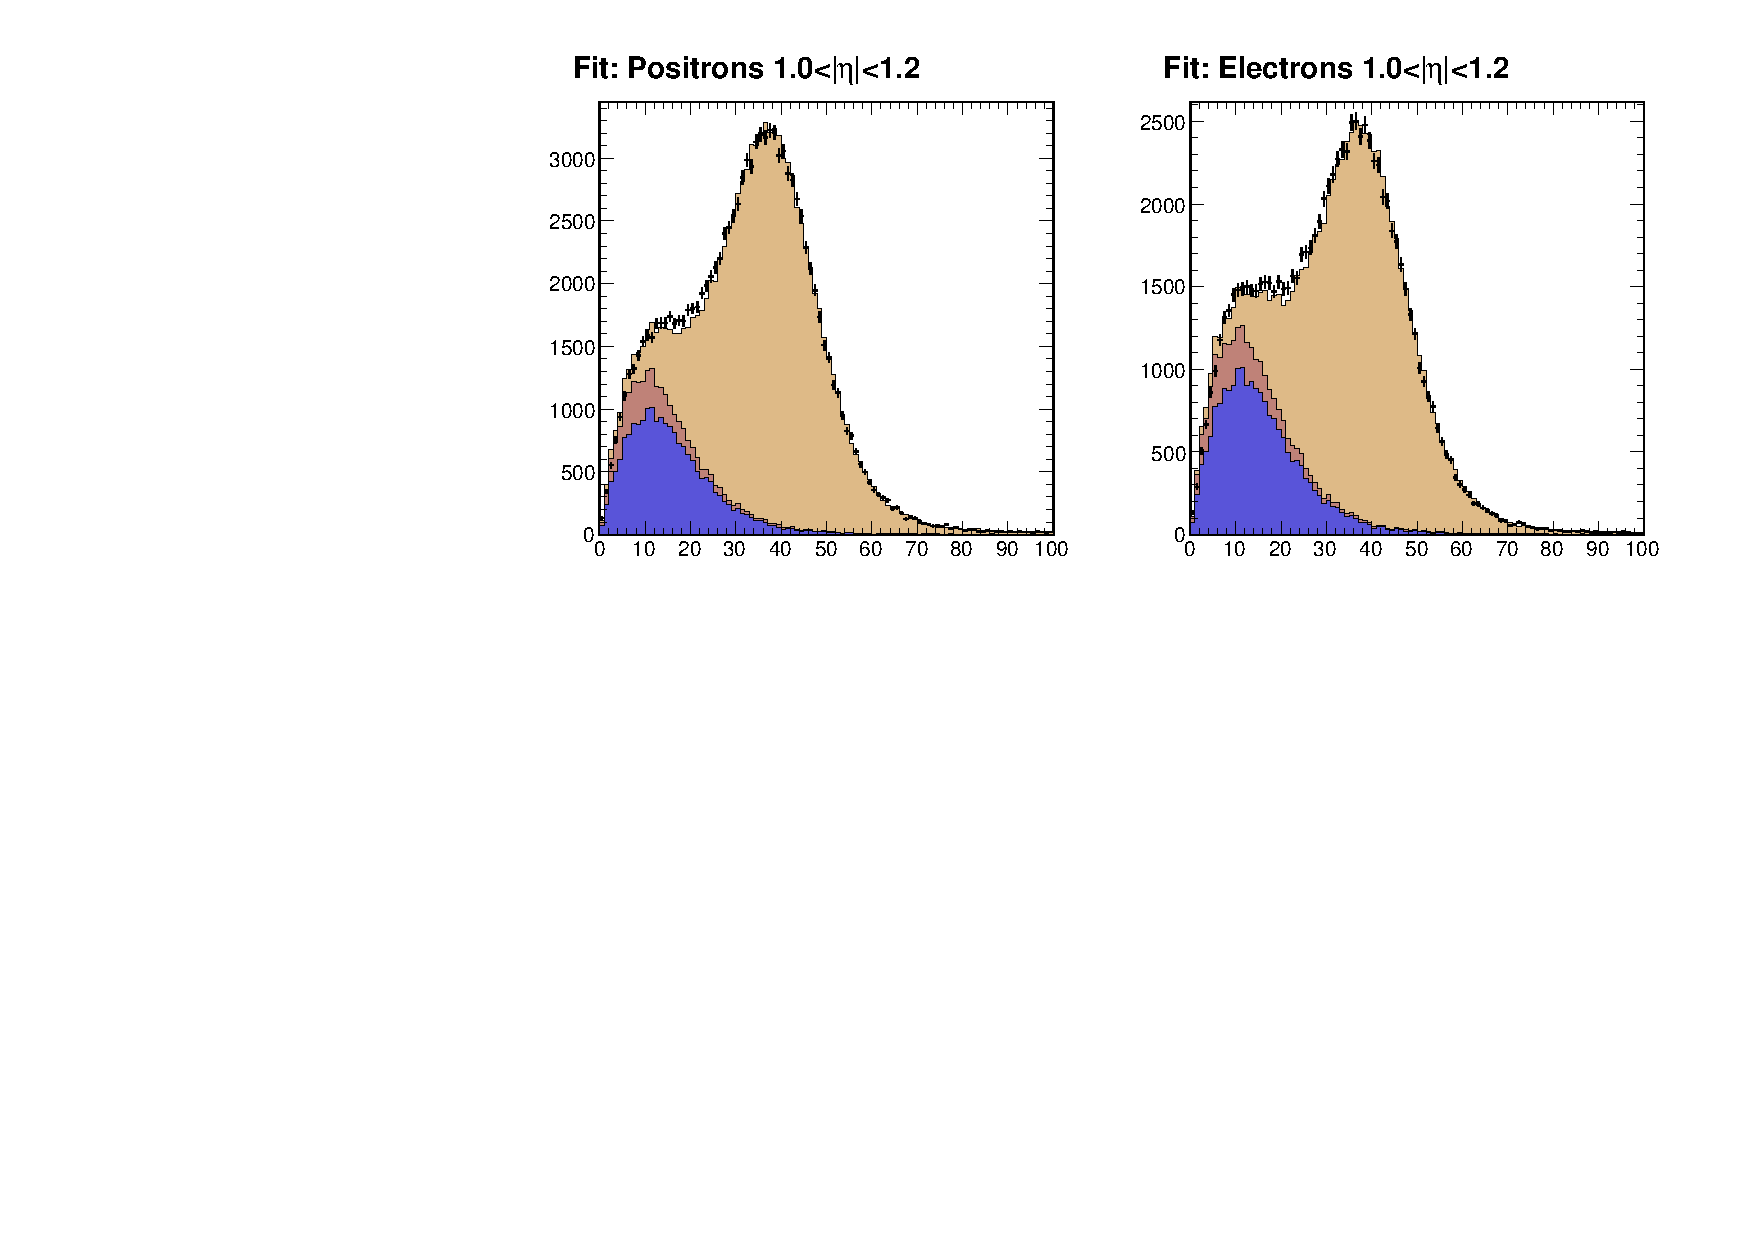
\includegraphics[width=0.95\textwidth]{data_5.pdf}
 \caption{  \label{fig:data2} The fit to \MET\ for eta bins 4,5 and 6.}
  \end{center}
\end{figure}

\begin{figure}
  \begin{center}
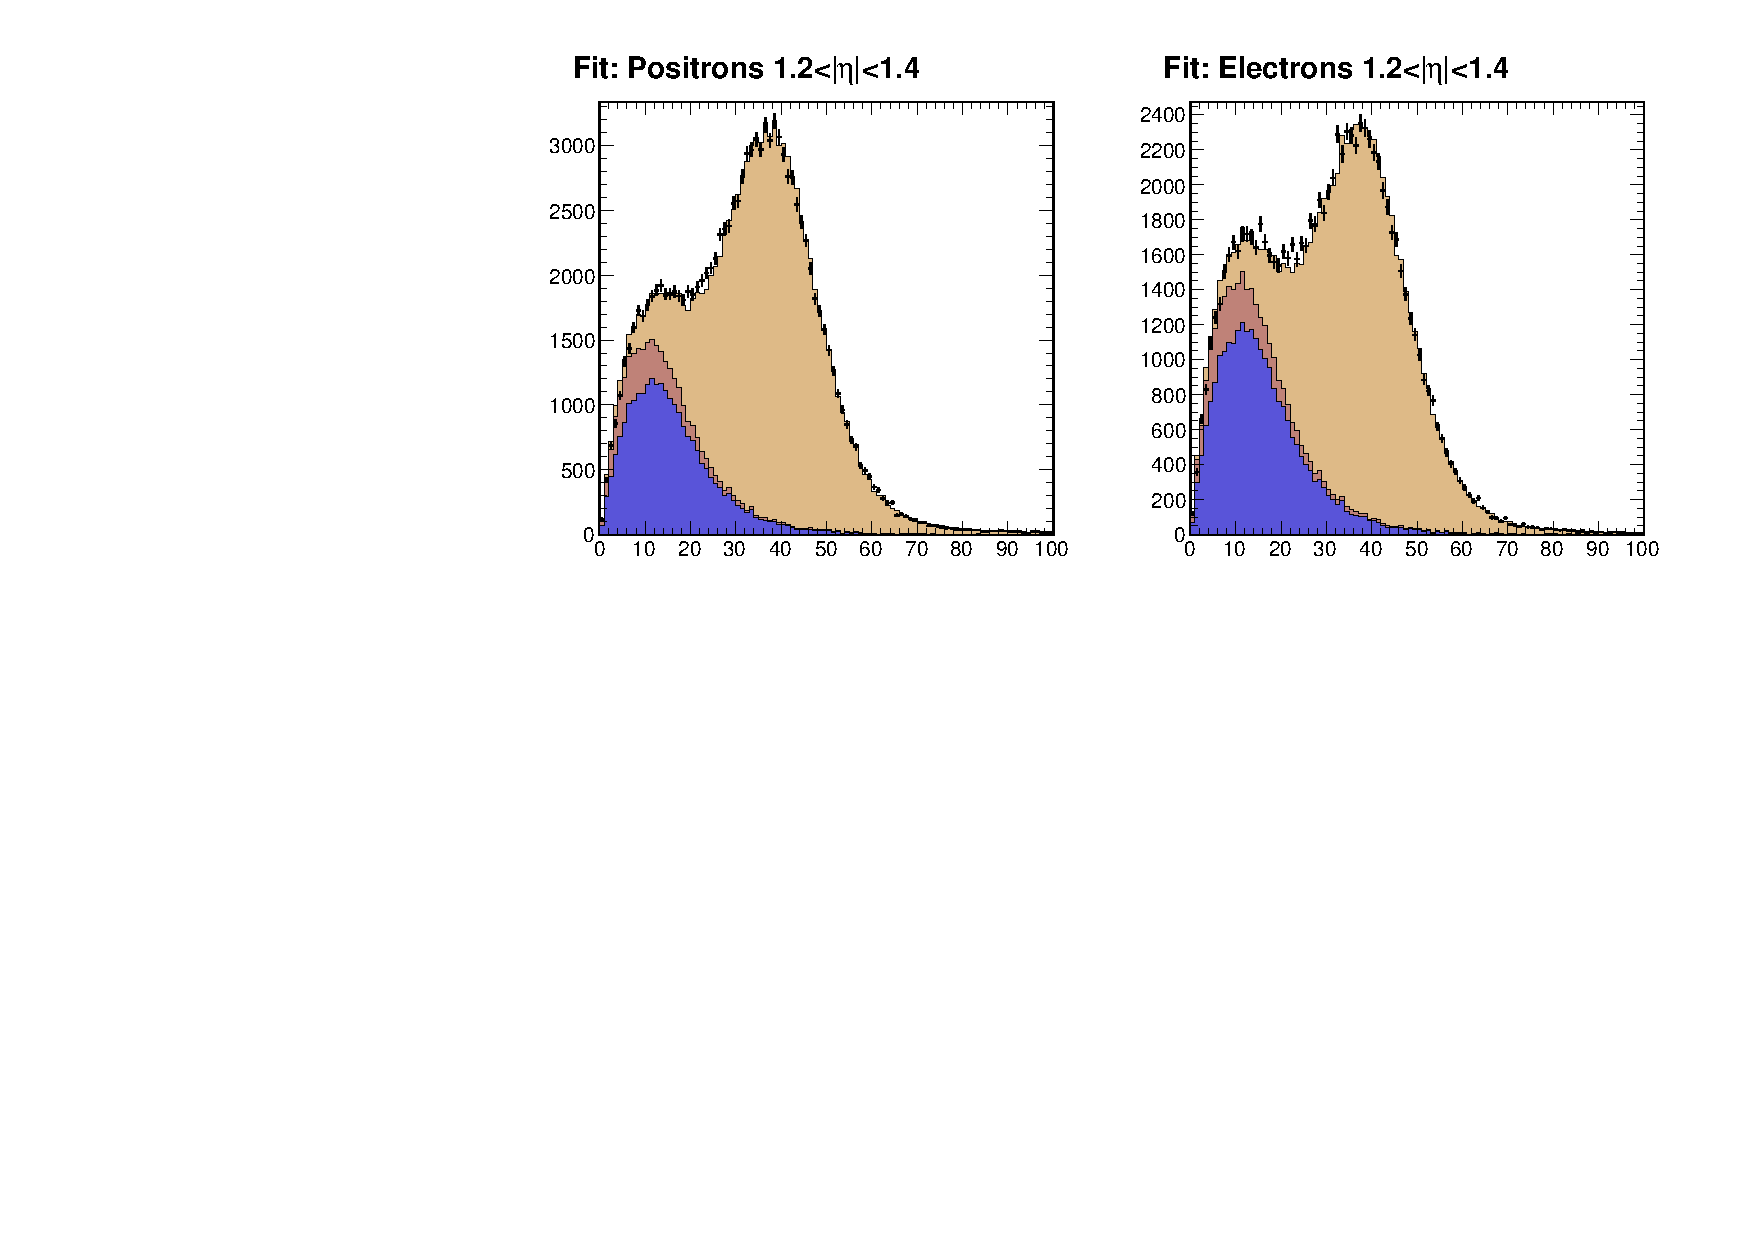
\includegraphics[width=0.95\textwidth]{data_6.pdf} \\
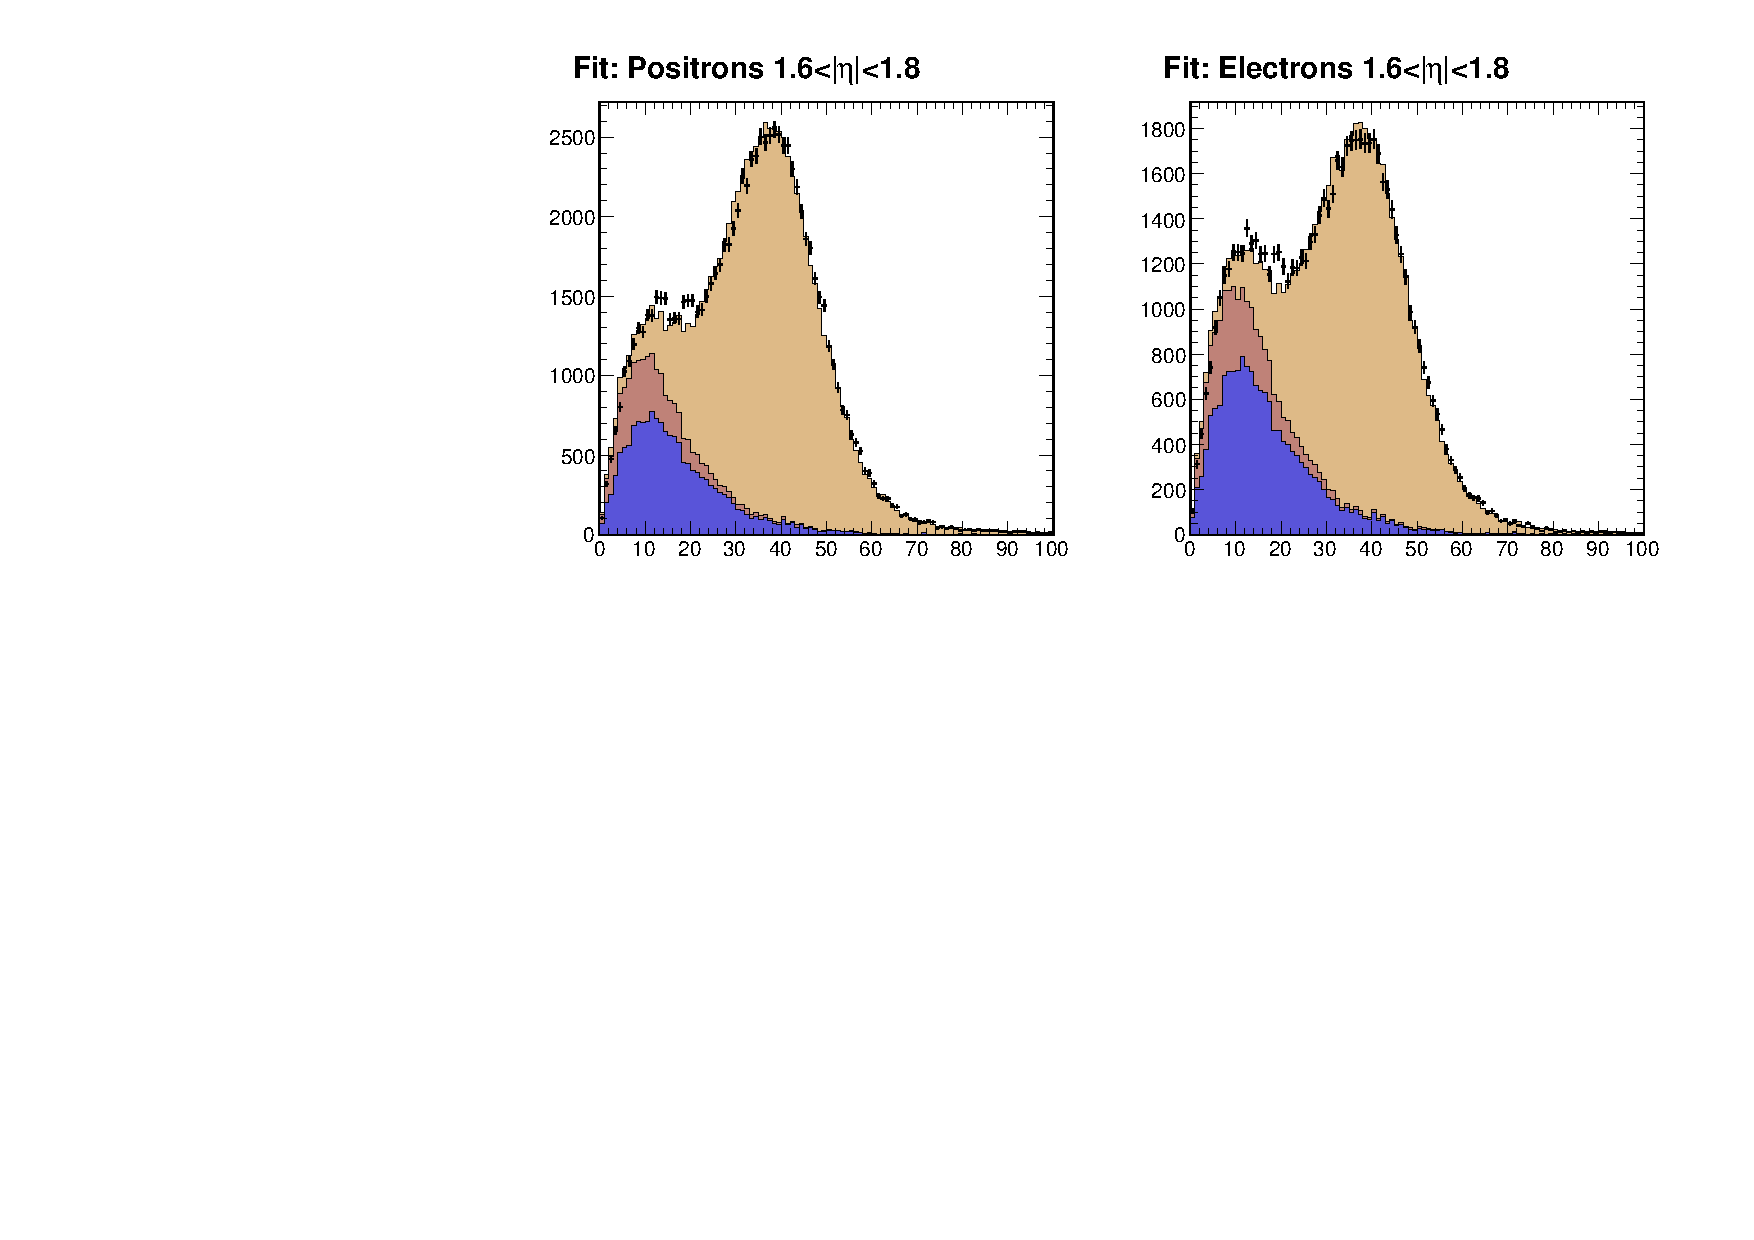
\includegraphics[width=0.95\textwidth]{data_7.pdf} \\
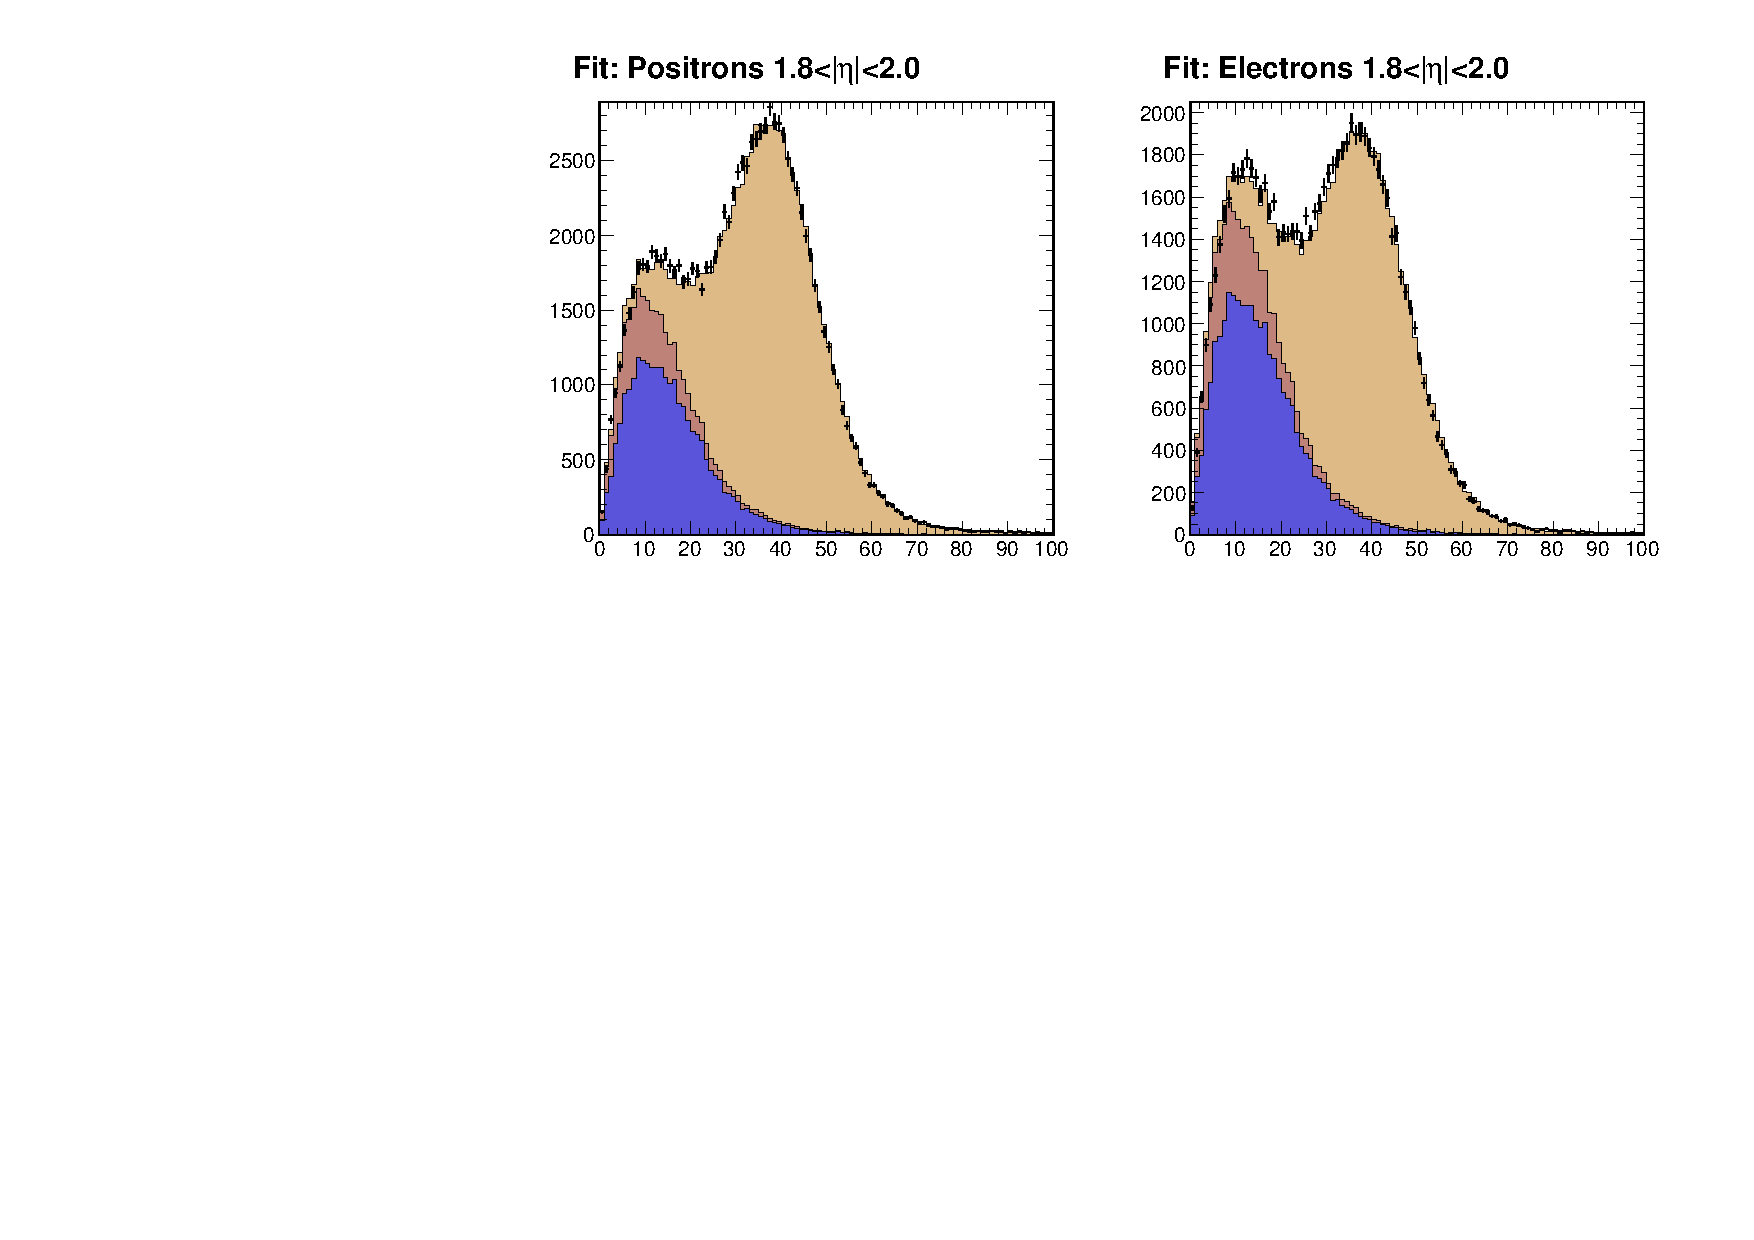
\includegraphics[width=0.95\textwidth]{data_8.pdf}
 \caption{  \label{fig:data3} The fit to \MET\ for eta bins 7,8 and 9.}
  \end{center}
\end{figure}

\begin{figure}
  \begin{center}
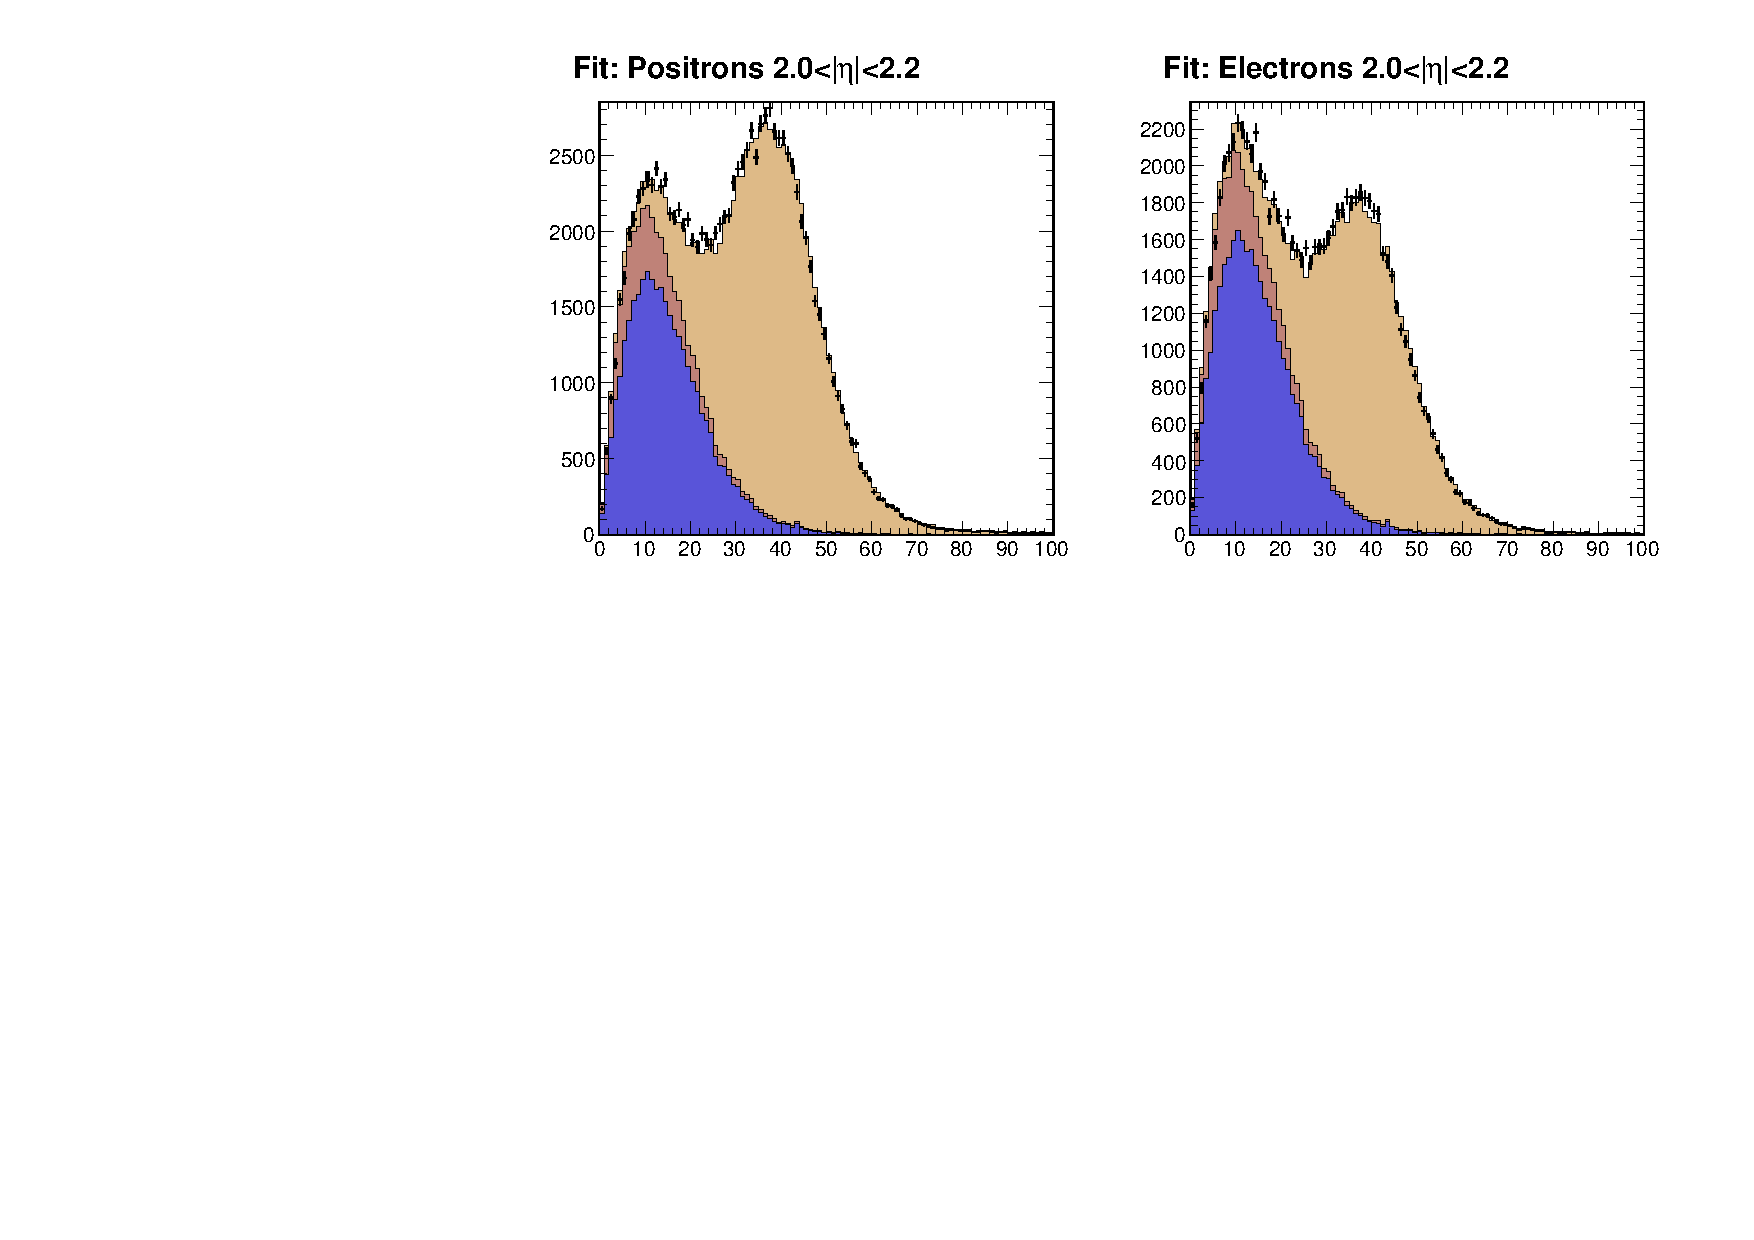
\includegraphics[width=0.95\textwidth]{data_9.pdf} \\
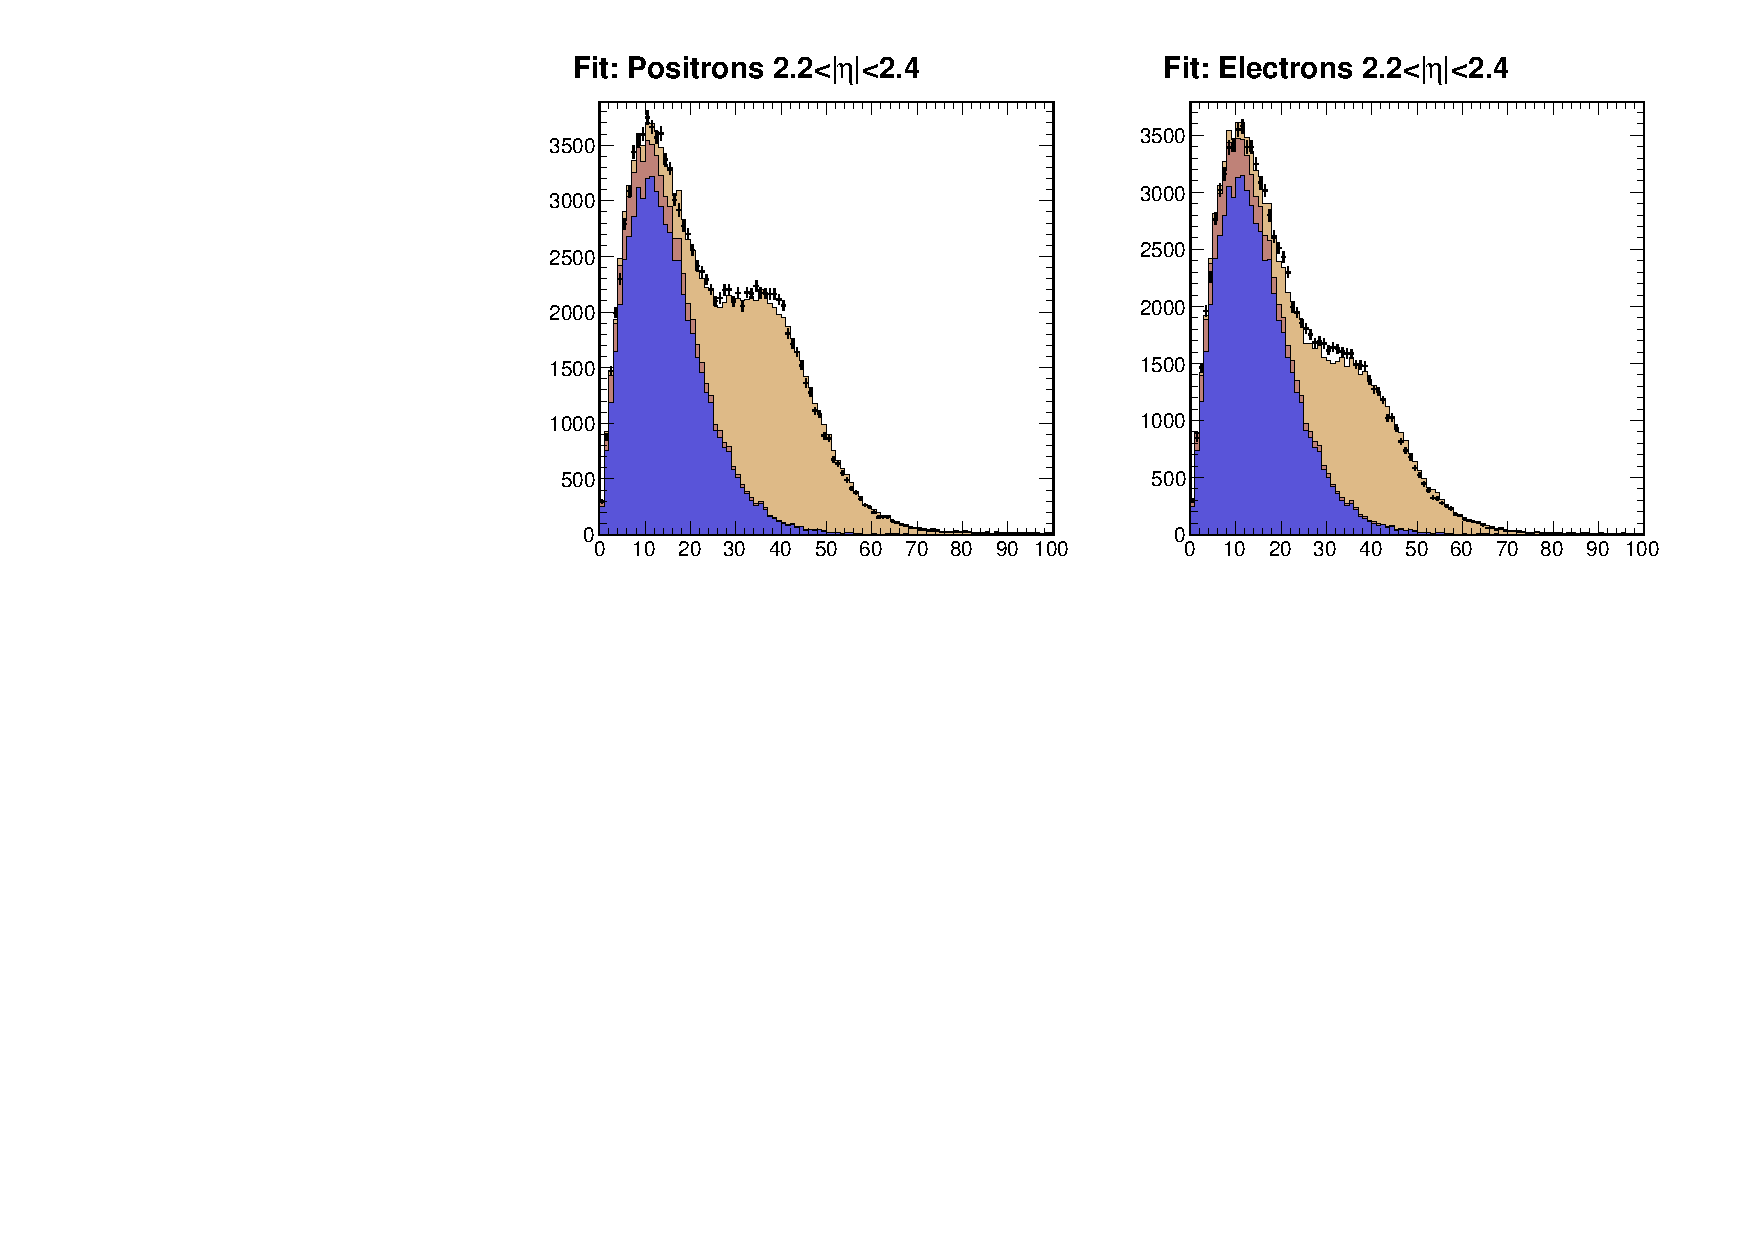
\includegraphics[width=0.95\textwidth]{data_10.pdf}
  \caption{  \label{fig:data4} The fit to \MET\ for eta bins 10 and 11.}
   \end{center}
\end{figure}

\begin{table}[htb]
 \begin{center}
 \begin{tabular}{lcrrrr}
$|\eta|$ range &  Charge &  N$_{QCD}$     & N$_{W\rightarrow e \nu}$  & N$_{W\rightarrow \tau \nu}$ & KS probability \\
               &         & fitted events & fitted events            & fitted events               & of fit \\
 \hline

$0.0<| \eta |<0.2$ &  +& $12794.5 \pm 202.6$ &$89698.3\pm330.5$&$ 1264.0\pm4.7 $&0.999 \\
                   &  -& $12926.1 \pm 194.3$ &$72369.8\pm297.6$&$ 1060.5\pm4.7 $&0.999 \\ 
$0.2<| \eta |<0.4$ &  +& $13773.9 \pm 209.6$ &$93109.0\pm337.7$&$ 1284.3\pm4.7 $&0.999 \\
                   &  -& $14071.4 \pm 199.8$ &$74215.4\pm302.0$&$ 1140.6\pm4.6 $&0.999 \\ 
$0.4<| \eta |<0.6$ &  +& $14803.9 \pm 212.9$ &$93211.7\pm338.1$&$ 1264.0\pm4.6 $&0.999 \\
                   &  -& $14554.2 \pm 203.5$ &$74360.3\pm303.4$&$ 1058.2\pm4.3 $&0.872 \\ 
$0.6<| \eta |<0.8$ &  +& $15484.5 \pm 217.0$ &$94943.5\pm341.0$&$ 1403.0\pm5.0 $&0.999 \\
                   &  -& $15523.8 \pm 206.4$ &$73764.2\pm302.2$&$ 1091.9\pm4.5 $&0.971 \\ 
$0.8<| \eta |<1.0$ &  +& $17177.5 \pm 221.7$ &$92971.3\pm338.1$&$ 1281.7\pm4.7 $&0.950 \\
                   &  -& $16871.6 \pm 210.5$ &$71476.6\pm298.3$&$ 1052.5\pm4.4 $&0.958 \\ 
$1.0<| \eta |<1.2$ &  +& $20001.2 \pm 229.9$ &$86449.0\pm329.0$&$ 1156.7\pm4.4 $&0.770 \\
                   &  -& $19930.1 \pm 218.4$ &$64643.8\pm286.6$&$ 957.0\pm4.2 $&0.676 \\ 
$1.2<| \eta |<1.4$ &  +& $24214.9 \pm 243.7$ &$83718.6\pm326.6$&$ 1115.6\pm4.4 $&0.985 \\
                   &  -& $24425.4 \pm 233.0$ &$60683.8\pm281.4$&$ 860.8\pm4.0 $&0.857 \\ 
$1.6<| \eta |<1.8$ &  +& $15759.0 \pm 228.6$ &$68726.0\pm302.3$&$ 939.0\pm4.1 $&0.480 \\
                   &  -& $16093.2 \pm 220.1$ &$47154.5\pm256.2$&$ 710.0\pm3.9 $&0.797 \\ 
$1.8<| \eta |<2.0$ &  +& $23809.6 \pm 241.7$ &$73116.7\pm305.0$&$ 908.4\pm3.8 $&0.915 \\
                   &  -& $23135.2 \pm 234.7$ &$49577.2\pm257.0$&$ 751.8\pm3.9 $&0.416 \\ 
$2.0<| \eta |<2.2$ &  +& $33773.0 \pm 261.7$ &$69872.7\pm299.1$&$ 846.4\pm3.6 $&0.581 \\
                   &  -& $32104.6 \pm 253.1$ &$45913.9\pm248.8$&$ 655.5\pm3.6 $&0.575 \\ 
$2.2<| \eta |<2.4$ &  +& $61794.8 \pm 309.3$ &$52495.9\pm269.8$&$ 607.9\pm3.1 $&0.386 \\
                   &  -& $60449.1 \pm 306.6$ &$34746.0\pm228.7$&$ 530.8\pm3.5 $&0.274 \\ 
 \end{tabular}
 \caption{\label{tab:chi2}
 Number of QCD events from the fitting procedure $\pm$ fit statistical uncertainty (Second column);
   Number of signal events  (Third column), Number of $W\rightarrow \tau \nu$ events (Fourth column),
 Kolmogorov-Smirnov probability (Fifth column).
 The quoted uncertainty for N$_{W\rightarrow e \nu}$ and N$_{W\rightarrow \tau \nu}$
 is the statistical uncertainty assigned to N$_{sig+EWK}$
 rescaled by the expected contribution of signal and $W\rightarrow \tau \nu$ in the signal+EWK template}
 \end{center}
\end{table}

\begin{table}[htb]
  \begin{center}
    \begin{tabular}{lc}
    $|\eta|$ range & $\mathcal{A}_{exp} (\times 10^{-3})$\\
    \hline
    $0.0<|\eta|<0.4$ & 106.9 $\pm$ 2.7\\
    $0.2<|\eta|<0.4$ & 112.9 $\pm$ 2.7\\
    $0.4<|\eta|<0.6$ & 112.5 $\pm$ 2.7\\
    $0.6<|\eta|<0.8$ & 125.5 $\pm$ 2.7\\
    $0.8<|\eta|<1.0$ & 130.7 $\pm$ 2.7\\
    $1.0<|\eta|<1.2$ & 144.3 $\pm$ 2.9\\
    $1.2<|\eta|<1.4$ & 159.5 $\pm$ 3.0 \\
    $1.6<|\eta|<1.8$ & 186.1 $\pm$ 3.4\\
    $1.8<|\eta|<2.0$ & 191.8 $\pm$ 3.2\\
    $2.0<|\eta|<2.2$ & 206.9 $\pm$ 3.3\\
    $2.2<|\eta|<2.4$ & 203.4 $\pm$ 4.1\\
    \end{tabular}
  \caption{\label{tab:uncorRes}Uncorrected values ($\times 10^{-3}$) of the
  charge asymmetry  for an integrated luminosity of \unit{840}{\invpb}. }
  \end{center}
\end{table}

\section{Corrections}
\todo[inline]{introduction to corrections}

\subsection{Relative Efficiency}
\todo[inline]{Relative efficiency systematic}


\begin{table}[htb]
\begin{center}
\begin{tabular}{lcrrrr}
$|\eta|$ range & Charge & $\epsilon_{GSF}$ &$\epsilon_{ID}$&$\epsilon_{HLT}$& R\\
\hline
$0.0<| \eta |<0.2$ &+& 98.5$\pm$0.2 &83.6$\pm$0.4 &97.9$\pm$0.2 &1.003$\pm$0.009\\
                   &-& 98.4$\pm$0.2 &83.5$\pm$0.5 &97.8$\pm$0.2 & \\
$0.2<| \eta |<0.4$ &+& 98.9$\pm$0.2 &82.6$\pm$0.5 &97.9$\pm$0.2 & 0.998$\pm$0.009\\
                   &-& 98.8$\pm$0.2 &82.8$\pm$0.5 &98.0$\pm$0.2 & \\
$0.4<| \eta |<0.6$ &+& 98.9$\pm$0.2&83.6$\pm$0.5 &98.1$\pm$0.2 & 0.995$\pm$0.009\\
                   &-& 99.0$\pm$0.2 &84.1$\pm$0.5 &97.9$\pm$0.2 & \\
$0.6<| \eta |<0.8$ &+& 98.7$\pm$0.2 &83.7$\pm$0.5 &98.4$\pm$0.2 & 0.999$\pm$0.009\\
                   &-& 98.7$\pm$0.2 &84.0$\pm$0.5&98.2$\pm$0.2 & \\
$0.8<| \eta |<1.0$ &+& 98.6$\pm$0.2 &84.3$\pm$0.5 &97.3$\pm$0.2 & 0.998$\pm$0.009\\
                   &-& 98.3$\pm$0.2 &84.4$\pm$0.5 &97.7$\pm$0.2 & \\
$1.0<| \eta |<1.2$ &+& 98.2$\pm$0.2 &82.6$\pm$0.5 &97.6$\pm$0.2 & 1.010$\pm$0.010\\
                   &-& 98.2$\pm$0.2 &81.7$\pm$0.5 &97.7$\pm$0.2 & \\
$1.2<| \eta |<1.4$ &+& 97.4$\pm$0.2 &79.4$\pm$0.5 &97.3$\pm$0.2 & 1.005$\pm$0.011\\
                   &-& 97.5$\pm$0.2 &78.8$\pm$0.6 &97.5$\pm$0.2 & \\
$1.6<| \eta |<1.8$ &+& 97.3$\pm$0.3 &62.3$\pm$0.7 &97.1$\pm$0.3 & 1.032$\pm$0.019\\
                   &-& 96.9$\pm$0.3 &61.2$\pm$0.7 &96.2$\pm$0.4 & \\
$1.8<| \eta |<2.0$ &+& 97.3$\pm$0.3 &62.1$\pm$0.8 &97.6$\pm$0.3 & 0.976$\pm$0.018\\
                   &-& 97.4$\pm$0.3 &63.7$\pm$0.8 &97.4$\pm$0.3 & \\
$2.0<| \eta |<2.2$ &+& 97.5$\pm$0.3 &58.6$\pm$0.9 &98.5$\pm$0.3 & 0.966$\pm$0.021\\
                   &-& 97.3$\pm$0.3 &60.7$\pm$0.8 &98.6$\pm$0.3 & \\
$2.2<| \eta |<2.4$ &+& 95.9$\pm$0.4 &55.1$\pm$1.0 &97.5$\pm$0.4 & 0.967$\pm$0.026\\
                   &-& 96.5$\pm$0.4 &56.3$\pm$1.0 &98.0$\pm$0.4 & \\

\hline
$0.0<| \eta |<1.4$ &+& 98.42$\pm$0.07 &82.9$\pm$0.2 &97.82$\pm$0.08 & 0.999$\pm$0.004\\
                   &-& 98.51$\pm$0.07 &82.9$\pm$0.2 &97.82$\pm$0.08 & \\
$1.6<| \eta |<2.4$ &+& 97.12$\pm$0.15 &60.1$\pm$0.4 &97.63$\pm$0.17 & 0.987$\pm$0.010\\
                   &-& 97.12$\pm$0.15 &61.0$\pm$0.4 &97.42$\pm$0.17 & \\
\hline
$0.0<| \eta |<2.4$ &+& 98.09$\pm$0.06 &77.41$\pm$0.17 &97.76$\pm$0.07 & 0.999$\pm$0.003\\
                   &-& 98.16$\pm$0.06 &77.49$\pm$0.17 &97.73$\pm$0.07 & \\
\end{tabular}
\end{center}
\caption{\label{tab:efficiency} GSF tracking, identification and HLT efficiency as a function of charge.}
\end{table}

\subsection{Charge Misassignment}
\todo[inline]{Misassignment of charge systermtic}
\begin{equation}
R_{ij}=\omega_i \times(1-\omega_j) + \omega_j \times(1-\omega_i)
\end{equation}

\begin{table}[htb]
  \begin{center}
\begin{tabular}{lr}
$\eta$ range        & $\omega \times 10^{-4}$    \\
\hline
$0.0<| \eta |<0.2$  & $ 1 \pm 1 $    \\ 
$0.2<| \eta |<0.4$  & $ 1 \pm 1 $    \\
$0.4<| \eta |<0.6$  & $ 1 \pm 1 $    \\
$0.6<| \eta |<0.8$  & $ 2 \pm 1 $    \\
$0.8<| \eta |<1.0$  & $ 4 \pm 2 $    \\ 
$1.0<| \eta |<1.2$  & $ 3 \pm 2 $    \\
$1.2<| \eta |<1.4$  & $ 3 \pm 2 $    \\
$1.6<| \eta |<1.8$  & $17 \pm 4 $    \\
$1.8<| \eta |<2.0$  & $12 \pm 4 $    \\
$2.0<| \eta |<2.2$  & $26 \pm 7 $    \\
$2.2<| \eta |<2.4$  & $ 7 \pm 7 $    \\
\end{tabular}
\caption{\label{tab:mischarge}Charge mismeasurement rate.}
\end{center}
\end{table}


\subsection{Lepton Energy Scale and Resolution}
\todo[inline]{Lepton energy scale and resolution systematic}



\begin{table}[htb]
  \begin{center}
    \begin{tabular}{ccccccc}
$\eta$ bin & $\sigma_{DATA}$ &  $\sigma_{MC}$ & $\sigma_{corr}$ & $k_{DATA}$ &  $k_{MC}$ & $k_{corr}$ \\
&GeV &GeV &GeV & & & \\
\hline
0.0$<|\eta|<$0.2 &1.08$\pm$ 0.03 & 0.83$\pm$ 0.03 & 0.70$\pm$ 0.06 & 1.0007$\pm$ 0.0003 & 1.0012$\pm$ 0.0003 & 0.9995$\pm$ 0.0004 \\ 
0.2$<|\eta|<$0.4 &1.01$\pm$ 0.03 & 0.85$\pm$ 0.02 & 0.54$\pm$ 0.07 & 1.0036$\pm$ 0.0003 & 1.0020$\pm$ 0.0003 & 1.0016$\pm$ 0.0004 \\ 
0.4$<|\eta|<$0.6 &1.16$\pm$ 0.03 & 0.95$\pm$ 0.02 & 0.67$\pm$ 0.06 & 1.0019$\pm$ 0.0003 & 1.0006$\pm$ 0.0003 & 1.0013$\pm$ 0.0004 \\ 
0.6$<|\eta|<$0.8 &1.16$\pm$ 0.03 & 0.98$\pm$ 0.02 & 0.61$\pm$ 0.07 & 1.0039$\pm$ 0.0003 & 1.0008$\pm$ 0.0003 & 1.0031$\pm$ 0.0004 \\ 
0.8$<|\eta|<$1.0 &1.28$\pm$ 0.03 & 1.13$\pm$ 0.02 & 0.61$\pm$ 0.08 & 1.0003$\pm$ 0.0004 & 0.9987$\pm$ 0.0003 & 1.0016$\pm$ 0.0005 \\ 
1.0$<|\eta|<$1.2 &1.68$\pm$ 0.03 & 1.42$\pm$ 0.02 & 0.90$\pm$ 0.07 & 0.9906$\pm$ 0.0004 & 0.9941$\pm$ 0.0003 & 0.9964$\pm$ 0.0005 \\ 
1.2$<|\eta|<$1.4 &2.02$\pm$ 0.03 & 1.62$\pm$ 0.02 & 1.21$\pm$ 0.06 & 0.9859$\pm$ 0.0005 & 0.9962$\pm$ 0.0004 & 0.9896$\pm$ 0.0006 \\ 
1.6$<|\eta|<$1.8 &2.78$\pm$ 0.04 & 2.26$\pm$ 0.03 & 1.62$\pm$ 0.08 & 0.9977$\pm$ 0.0007 & 0.9797$\pm$ 0.0005 & 1.0184$\pm$ 0.0009 \\ 
1.8$<|\eta|<$2.0 &2.38$\pm$ 0.04 & 1.83$\pm$ 0.03 & 1.53$\pm$ 0.07 & 0.9976$\pm$ 0.0006 & 0.9768$\pm$ 0.0005 & 1.0213$\pm$ 0.0008 \\ 
2.0$<|\eta|<$2.2 &2.16$\pm$ 0.04 & 1.49$\pm$ 0.03 & 1.56$\pm$ 0.06 & 0.9922$\pm$ 0.0006 & 0.9837$\pm$ 0.0005 & 1.0087$\pm$ 0.0008 \\ 
2.2$<|\eta|<$2.4 &2.21$\pm$ 0.04 & 1.39$\pm$ 0.04 & 1.72$\pm$ 0.06 & 0.9510$\pm$ 0.0008 & 0.9881$\pm$ 0.0005 & 0.9625$\pm$ 0.0009 \\ 

    \end{tabular}
    \caption{\label{tab:ResCorr}Scale and residual smearing factor obtained with $Z\rightarrow ee$ sample}
  \end{center}
\end{table}

\begin{figure}[htb]
  \begin{center}
\includegraphics*[width=0.45\textwidth]{ENSmeChargeSep.png}
\includegraphics*[width=0.45\textwidth]{ENKfactChargeSep.png}
 \caption{\label{Scale_sep} $\sigma_{corr}$(left) and $k_{corr}$(right) for electrons and positrons.}
\end{center}
\end{figure}

\begin{table}[htb]
  \begin{center}
    \begin{tabular}{cccccc}
$\eta$ range & Correction  & Stat.   &PDF  Syst. &  FSR Syst. & Scale Syst.\\
          & factor & Error & Error   & Error  & Error  \\
     \hline
 $0.0<|\eta|<0.2$ & -1.1 & 0.1 & 0.3  &0.1 & 0.0\\
 $0.2<|\eta|<0.4$ &  0.2 & 0.1 & 0.6  &0.0 & 0.0\\
 $0.4<|\eta|<0.6$ & -0.4 & 0.1 & 0.3  &0.0 & 0.0\\
 $0.6<|\eta|<0.8$ & -0.9 & 0.1 & 0.3  &0.0 & 0.0\\
 $0.8<|\eta|<1.0$ & -0.9 & 0.1 & 0.6  &0.0 & 0.0\\
 $1.0<|\eta|<1.2$ & -1.4 & 0.1 & 1.0  &0.0 & 0.0\\
 $1.2<|\eta|<1.4$ & -3.5 & 0.1 & 0.8  &0.0 & 0.1\\
 $1.6<|\eta|<1.8$ & -2.5 & 0.1 & 0.8  &0.0 & 0.0\\
 $1.8<|\eta|<2.0$ & -4.4 & 0.1 & 1.6  &0.0 & 0.0\\
 $2.0<|\eta|<2.2$ & -0.2 & 0.1 & 2.6  &0.0 & 0.1\\
 $2.2<|\eta|<2.4$ & -3.5 & 0.1 & 2.4  &0.0 & 0.2\\
    \end{tabular}
    \caption{\label{tab:acc}Bias in the charge asymmetry introduced by the the electron energy scale and resolution.
 All values are in units $\times 10^{-3}$}
  \end{center}
\end{table}

\begin{table}[htb]
  \begin{center}
    \begin{tabular}{l | c c c c c c c c c c c}
& \scriptsize{$\left[0.0,0.2\right]$}
& \scriptsize{$\left[0.2,0.4\right]$}
& \scriptsize{$\left[0.4,0.6\right]$}
& \scriptsize{$\left[0.6,0.8\right]$}
& \scriptsize{$\left[0.8,1.0\right]$}
& \scriptsize{$\left[1.0,1.2\right]$}
& \scriptsize{$\left[1.2,1.4\right]$}
& \scriptsize{$\left[1.6,1.8\right]$}
& \scriptsize{$\left[1.8,2.0\right]$}
& \scriptsize{$\left[2.0,2.2\right]$}
& \scriptsize{$\left[2.2,2.4\right]$} \\ \hline

\scriptsize{$\left[0.0,0.2\right]$} &0.10 & 0.06 & 0.07 & 0.07 & 0.14 & 0.20 & 0.15 & 0.18 & 0.43 & 0.61 & 0.58 \\
\scriptsize{$\left[0.2,0.4\right]$} &0.06 & 0.42 & 0.13 & 0.08 & 0.18 & 0.26 & 0.17 & 0.17 & 0.45 & 1.02 & 0.66 \\
\scriptsize{$\left[0.4,0.6\right]$} &0.07 & 0.13 & 0.09 & 0.07 & 0.13 & 0.17 & 0.13 & 0.15 & 0.33 & 0.57 & 0.52 \\
\scriptsize{$\left[0.6,0.8\right]$} &0.07 & 0.08 & 0.07 & 0.06 & 0.12 & 0.18 & 0.13 & 0.15 & 0.32 & 0.51 & 0.52 \\
\scriptsize{$\left[0.8,1.0\right]$} &0.14 & 0.18 & 0.13 & 0.12 & 0.31 & 0.43 & 0.29 & 0.34 & 0.76 & 1.21 & 1.13 \\
\scriptsize{$\left[1.0,1.2\right]$} &0.20 & 0.26 & 0.17 & 0.18 & 0.43 & 1.02 & 0.60 & 0.61 & 1.25 & 2.30 & 2.16 \\
\scriptsize{$\left[1.2,1.4\right]$} &0.15 & 0.17 & 0.13 & 0.13 & 0.29 & 0.60 & 0.60 & 0.49 & 0.89 & 1.74 & 1.70 \\
\scriptsize{$\left[1.6,1.8\right]$} &0.18 & 0.17 & 0.15 & 0.15 & 0.34 & 0.61 & 0.49 & 0.57 & 1.00 & 1.71 & 1.64 \\
\scriptsize{$\left[1.8,2.0\right]$} &0.43 & 0.45 & 0.33 & 0.32 & 0.76 & 1.25 & 0.89 & 1.00 & 2.61 & 3.56 & 3.30 \\
\scriptsize{$\left[2.0,2.2\right]$} &0.61 & 1.02 & 0.57 & 0.51 & 1.21 & 2.30 & 1.74 & 1.71 & 3.56 & 6.79 & 5.88 \\
\scriptsize{$\left[2.2,2.4\right]$} &0.58 & 0.66 & 0.52 & 0.52 & 1.13 & 2.16 & 1.70 & 1.64 & 3.30 & 5.88 & 5.95 \\
    \end{tabular}
    \caption{\label{tab:covMatrix}Error Correlation Matrix ($\times 10^{-6}$).}
  \end{center}
\end{table}



\subsection{Correction Factors}
\todo[inline]{summary of corrections to measurment}

\begin{table}[htb]
  \begin{center}
    \begin{tabular}{ccccc}
$\eta$ range & $\mathcal{A}_M$ & Rel. Eff & Energy & $\mathcal{A}_C$ \\
& & MisCharge & Resolution &  \\
& & Correction  & Correction & \\
\hline
 $0.0<|\eta|<0.4$ & 106.9 &-1.5$\pm$ 4.5 & -1.1$\pm$0.3 & 104.3\\ 
 $0.2<|\eta|<0.4$ & 112.9 &+1.0$\pm$ 4.4 &  0.2$\pm$0.6 & 114.1\\ 
 $0.4<|\eta|<0.6$ & 112.5 &+2.5$\pm$ 4.4 & -0.4$\pm$0.3 & 114.6\\
 $0.6<|\eta|<0.8$ & 125.5 &+0.5$\pm$ 4.4 & -0.9$\pm$0.3 & 125.1\\ 
 $0.8<|\eta|<1.0$ & 130.7 &+0.2$\pm$ 4.4 & -0.9$\pm$0.6 & 130.0\\ 
 $1.0<|\eta|<1.2$ & 144.3 &-4.8$\pm$ 4.9 & -1.4$\pm$1.0 & 138.1\\ 
 $1.2<|\eta|<1.4$ & 159.5 &-2.3$\pm$ 5.4 & -3.5$\pm$0.8 & 153.7\\ 
 $1.6<|\eta|<1.8$ & 186.1 &-14.9$\pm$ 9.2 & -2.5$\pm$0.8 & 168.7\\
 $1.8<|\eta|<2.0$ & 191.8 &+12.0$\pm$ 8.7 & -4.4$\pm$1.6 & 199.5\\
 $2.0<|\eta|<2.2$ & 206.9 &+17.4$\pm$10.1&  -0.2$\pm$2.6 & 224.1\\
 $2.2<|\eta|<2.4$ & 203.4 &+16.1$\pm$12.5 & -3.5$\pm$2.4 & 216.0\\

    \end{tabular}
    \caption{\label{tab:CorrectionFactors}Correction factors ($\times 10~{-3}$) applied to the measured asymmetry}
  \end{center}
\end{table}


\section{Systematic Uncertainties}
\todo[inline]{Systematic uncertainties for 840 measurement.}
sample text sample text sample text sample text sample text sample text sample
text sample text sample text sample text sample text sample text sample text
sample text sample text sample text sample text sample text sample text sample
text sample text sample text sample text sample text sample text sample text

\subsection{Signal Extraction Method}
\todo[inline]{Systematic uncertainties for signal extraction method.}
sample text sample text sample text sample text sample text sample text sample
text sample text sample text sample text sample text sample text sample text
sample text sample text sample text sample text sample text sample text sample
text sample text sample text sample text sample text sample text sample text

\subsubsection{QCD \ETm Shape}
\todo[inline]{Systematic uncertainties for qcd met shape.}
sample text sample text sample text sample text sample text sample text sample
text sample text sample text sample text sample text sample text sample text
sample text sample text sample text sample text sample text sample text sample
text sample text sample text sample text sample text sample text sample text
sample text sample text sample text sample text sample text sample text sample
text sample text sample text sample text sample text sample text sample text


\begin{table}[htb]
\begin{center}
\begin{tabular}{cr}
$|\eta|$ range  & $\sigma(\mathcal{A}) \times 10^{-3}$\\
\hline
$0.0<|\eta|<0.2$ & 1.0\\
$0.2<|\eta|<0.4$ & 1.9\\
$0.4<|\eta|<0.6$ & 2.2\\
$0.6<|\eta|<0.8$ & 1.8\\
$0.8<|\eta|<1.0$ & 0.5\\
$1.0<|\eta|<1.2$ & 1.5\\
$1.2<|\eta|<1.4$ & 1.4\\
$1.6<|\eta|<1.8$ & 2.5\\
$1.8<|\eta|<2.0$ & 1.3\\
$2.0<|\eta|<2.2$ & 0.6\\
$2.2<|\eta|<2.4$ & 1.6\\
\end{tabular}
\caption{Maximum distance between the asymmetry measured with many different antiselections
and the asymmetry measured with the chosen antiselection in MC pseudo data and real data for each eta bin.}
\label{tab:systQCD}
\end{center}
\end{table}

\subsubsection{Signal \ETm Shape from Boson Recoil}
\todo[inline]{Systematic uncertainties for signal met shape.}
sample text sample text sample text sample text sample text sample text sample
text sample text sample text sample text sample text sample text sample text
sample text sample text sample text sample text sample text sample text sample
text sample text sample text sample text sample text sample text sample text
sample text sample text sample text sample text sample text sample text sample
text sample text sample text sample text sample text sample text sample text

\begin{table}[htb]
\begin{center}
\begin{tabular}{crrr}
$|\eta|$  & \multicolumn{3}{c}{$\sigma(\mathcal{A}) \times 10^{-3}$}\\
range     & Recoil Corr.& PDF & Combined \\
\hline
$0.0<|\eta|<0.2$ &  0.2 &  1.5  & 1.5 \\
$0.2<|\eta|<0.4$ &  0.4 &  1.6  & 1.7 \\
$0.4<|\eta|<0.6$ &  0.6 &  1.3  & 1.4 \\
$0.6<|\eta|<0.8$ &  0.8 &  1.5  & 1.7 \\
$0.8<|\eta|<1.0$ &  0.9 &  1.6  & 1.8 \\
$1.0<|\eta|<1.2$ &  0.8 &  1.7  & 1.9 \\
$1.2<|\eta|<1.4$ &  1.5 &  1.6  & 2.3 \\
$1.6<|\eta|<1.8$ &  0.7 &  1.7  & 1.9 \\
$1.8<|\eta|<2.0$ &  0.4 &  1.5  & 1.6 \\
$2.0<|\eta|<2.2$ &  1.1 &  1.5  & 1.9 \\
$2.2<|\eta|<2.4$ &  0.9 &  2.3  & 2.4 \\
\end{tabular}
\caption{\label{tab:systSIG}Systematic uncertainty due to the Signal \MET shape
used in the signal extraction method assigned to each eta bin.}
\end{center}
\end{table}

\subsubsection{EWK \ETm Shape}
\todo[inline]{Systematic uncertainties for EWK met shape.}
sample text sample text sample text sample text sample text sample text sample
sample text sample text sample text sample text sample text sample text sample
sample text sample text sample text sample text sample text sample text sample
sample text sample text sample text sample text sample text sample text sample
text sample text sample text sample text sample text sample text sample text
text sample text sample text sample text sample text sample text sample text
text sample text sample text sample text sample text sample text sample text
text sample text sample text sample text sample text sample text sample text

\begin{table}[htb]
\begin{center}
\begin{tabular}{cr}
\hline
$|\eta|$ range & $\sigma(\mathcal{A}) \times 10^{-3}$\\
\hline
\hline
$0.0<|\eta|<0.2$ & 0.0\\
$0.2<|\eta|<0.4$ & 0.0\\
$0.4<|\eta|<0.6$ & 0.0\\
$0.6<|\eta|<0.8$ & 0.0\\
$0.8<|\eta|<1.0$ & 0.0\\
$1.0<|\eta|<1.2$ & 0.0\\
$1.2<|\eta|<1.4$ & 0.0\\
$1.6<|\eta|<1.8$ & 0.0\\
$1.8<|\eta|<2.0$ & 0.0\\
$2.0<|\eta|<2.2$ & 0.0\\
$2.2<|\eta|<2.4$ & 0.0\\
\hline
\end{tabular}
\caption{\label{tab:systEWK}Systematic uncertainty due to the electroweak \MET shape used in the signal extraction method assigned to each eta bin.}
\end{center}
\end{table}


\begin{table}[tb]
   \begin{center}
      \begin{tabular}{l|ccccccccccc}

& \scriptsize{$\left[0.0,0.2\right]$}
& \scriptsize{$\left[0.2,0.4\right]$}
& \scriptsize{$\left[0.4,0.6\right]$}
& \scriptsize{$\left[0.6,0.8\right]$}
& \scriptsize{$\left[0.8,1.0\right]$}
& \scriptsize{$\left[1.0,1.2\right]$}
& \scriptsize{$\left[1.2,1.4\right]$}
& \scriptsize{$\left[1.6,1.8\right]$}
& \scriptsize{$\left[1.8,2.0\right]$}
& \scriptsize{$\left[2.0,2.2\right]$}
& \scriptsize{$\left[2.2,2.4\right]$} \\ \hline

\scriptsize{$\left[0.0,0.2\right]$}& 3.33& 2.54& 2.17& 2.45& 2.60& 2.73& 2.72& 2.73& 2.33& 2.51& 3.65 \\
\scriptsize{$\left[0.2,0.4\right]$}& 2.54& 6.42& 2.47& 2.78& 2.95& 3.07& 3.19& 3.06& 2.55& 2.90& 4.07 \\
\scriptsize{$\left[0.4,0.6\right]$}& 2.17& 2.47& 7.14& 2.53& 2.67& 2.74& 3.03& 2.73& 2.18& 2.71& 3.58 \\
\scriptsize{$\left[0.6,0.8\right]$}& 2.45& 2.78& 2.53& 6.17& 3.14& 3.21& 3.62& 3.15& 2.51& 3.17& 4.19 \\
\scriptsize{$\left[0.8,1.0\right]$}& 2.60& 2.95& 2.67& 3.14& 3.63& 3.45& 3.92& 3.37& 2.68& 3.41& 4.50 \\
\scriptsize{$\left[1.0,1.2\right]$}& 2.73& 3.07& 2.74& 3.21& 3.45& 5.79& 3.93& 3.47& 2.80& 3.45& 4.64 \\
\scriptsize{$\left[1.2,1.4\right]$}& 2.72& 3.19& 3.03& 3.62& 3.92& 3.93& 6.78& 3.79& 2.86& 4.07& 5.04 \\
\scriptsize{$\left[1.6,1.8\right]$}& 2.73& 3.06& 2.73& 3.15& 3.37& 3.47& 3.79& 9.67& 2.78& 3.36& 4.56 \\
\scriptsize{$\left[1.8,2.0\right]$}& 2.33& 2.55& 2.18& 2.51& 2.68& 2.80& 2.86& 2.78& 4.04& 2.60& 3.73 \\
\scriptsize{$\left[2.0,2.2\right]$}& 2.51& 2.90& 2.71& 3.17& 3.41& 3.45& 4.07& 3.36& 2.60& 3.86& 4.46 \\
\scriptsize{$\left[2.2,2.4\right]$}& 3.65& 4.07& 3.58& 4.19& 4.50& 4.64& 5.04& 4.56& 3.73& 4.46& 8.67 \\

      \end{tabular}
    \end{center}
  \caption{\label{tab_corr_fit}Error correlation matrix for the fitting procedure. All the values are given in units $\times 10^{-6}$ }
\end{table}

\subsection{Systematic Uncertainty Summary}
\todo[inline]{Summary of systematic uncertainties for 840 measurement.}
sample text sample text sample text sample text sample text sample text sample
text sample text sample text sample text sample text sample text sample text
sample text sample text sample text sample text sample text sample text sample
text sample text sample text sample text sample text sample text sample text
sample text sample text sample text sample text sample text sample text sample
text sample text sample text sample text sample text sample text sample text
sample text sample text sample text sample text sample text sample text sample
text sample text sample text sample text sample text sample text sample text
sample text sample text sample text sample text sample text sample text sample
text sample text sample text sample text sample text sample text sample text

\begin{table}[tb]
 \begin{center}
   \begin{tabular}{lcccc}
      &Signal & Energy & Charge &  Efficiency \\
     & Yield & Scale and Res. & MisId. & Ratio \\ \hline
$0.0<|\eta|<0.2$ & 1.8 & 0.6 & 0.0 &  4.5 \\
$0.2<|\eta|<0.4$ & 2.5 & 0.6 & 0.0 &  4.4 \\
$0.4<|\eta|<0.6$ & 2.7 & 0.3 & 0.0 &  4.4 \\
$0.6<|\eta|<0.8$ & 2.5 & 0.3 & 0.0 &  4.4 \\
$0.8<|\eta|<1.0$ & 1.9 & 0.6 & 0.1 &  4.4 \\
$1.0<|\eta|<1.2$ & 2.4 & 1.0 & 0.1 &  4.9 \\
$1.2<|\eta|<1.4$ & 2.6 & 0.8 & 0.1 &  5.4 \\
$1.6<|\eta|<1.8$ & 3.1 & 0.8 & 0.1 &  9.2 \\
$1.8<|\eta|<2.0$ & 2.0 & 1.6 & 0.2 &  8.7 \\
$2.0<|\eta|<2.2$ & 2.0 & 2.6 & 0.3 & 10.0 \\
$2.2<|\eta|<2.4$ & 2.9 & 2.4 & 0.3 & 12.5 \\
    \end{tabular}
  \end{center}
 \caption{\label{tab:summarysyst}Summary of the systematic uncertainties. All values are in units $\times 10^{-3}$. }
\end{table}
                  

\begin{table}[tb]
   \begin{center}
      \begin{tabular}{l|ccccccccccc}
& \scriptsize{$\left[0.0,0.2\right]$}
& \scriptsize{$\left[0.2,0.4\right]$}
& \scriptsize{$\left[0.4,0.6\right]$}
& \scriptsize{$\left[0.6,0.8\right]$}
& \scriptsize{$\left[0.8,1.0\right]$}
& \scriptsize{$\left[1.0,1.2\right]$}
& \scriptsize{$\left[1.2,1.4\right]$}
& \scriptsize{$\left[1.6,1.8\right]$}
& \scriptsize{$\left[1.8,2.0\right]$}
& \scriptsize{$\left[2.0,2.2\right]$}
& \scriptsize{$\left[2.2,2.4\right]$} \\ \hline

\scriptsize{$\left[0.0,0.2\right]$} & 23.7 & 2.6 & 2.2 & 2.5 & 2.7 & 2.9 & 2.9 & 2.9 & 2.8 & 3.1 & 4.2 \\
\scriptsize{$\left[0.2,0.4\right]$} & 2.6 & 26.2 & 2.6 & 2.9 & 3.1 & 3.3 & 3.4 & 3.2 & 3.0 & 3.9 & 4.7 \\
\scriptsize{$\left[0.4,0.6\right]$} & 2.2 & 2.6 & 26.6 & 2.6 & 2.8 & 2.9 & 3.2 & 2.9 & 2.5 & 3.3 & 4.1 \\
\scriptsize{$\left[0.6,0.8\right]$} & 2.5 & 2.9 & 2.6 & 25.6 & 3.3 & 3.4 & 3.7 & 3.3 & 2.8 & 3.7 & 4.7 \\
\scriptsize{$\left[0.8,1.0\right]$} & 2.7 & 3.1 & 2.8 & 3.3 & 23.3 & 3.9 & 4.2 & 3.7 & 3.4 & 4.6 & 5.6 \\
\scriptsize{$\left[1.0,1.2\right]$} & 2.9 & 3.3 & 2.9 & 3.4 & 3.9 & 30.8 & 4.5 & 4.1 & 4.0 & 5.7 & 6.8 \\
\scriptsize{$\left[1.2,1.4\right]$} & 2.9 & 3.4 & 3.2 & 3.7 & 4.2 & 4.5 & 36.5 & 4.3 & 3.7 & 5.8 & 6.7 \\
\scriptsize{$\left[1.6,1.8\right]$} & 2.9 & 3.2 & 2.9 & 3.3 & 3.7 & 4.1 & 4.3 & 94.9 & 3.8 & 5.1 & 6.2 \\
\scriptsize{$\left[1.8,2.0\right]$} & 2.8 & 3.0 & 2.5 & 2.8 & 3.4 & 4.0 & 3.7 & 3.8 & 82.4 & 6.2 & 7.0 \\
\scriptsize{$\left[2.0,2.2\right]$} & 3.1 & 3.9 & 3.3 & 3.7 & 4.6 & 5.7 & 5.8 & 5.1 & 6.2 & 110.7 & 10.3 \\
\scriptsize{$\left[2.2,2.4\right]$} & 4.2 & 4.7 & 4.1 & 4.7 & 5.6 & 6.8 & 6.7 & 6.2 & 7.0 & 10.3 & 171.0 \\

    \end{tabular}
    \end{center}
  \caption{\label{tab_corr_tot}Correlation matrix for all the systematic errors.
                               All the values are given in units $\times 10^{-6}$ }
\end{table}



\section{Results}

\todo[inline]{Summarise results of the 840pb result.}

sample text sample text sample text sample text sample text sample text sample
text sample text sample text sample text sample text sample text sample text
sample text sample text sample text sample text sample text sample text sample
text sample text sample text sample text sample text sample text sample text
sample text sample text sample text sample text sample text sample text sample
text sample text sample text sample text sample text sample text sample text
sample text sample text sample text sample text sample text sample text sample
text sample text sample text sample text sample text sample text sample text
sample text sample text sample text sample text sample text sample text sample
text sample text sample text sample text sample text sample text sample text
sample text sample text sample text sample text sample text sample text sample
text sample text sample text sample text sample text sample text sample text
sample text sample text sample text sample text sample text sample text sample
text sample text sample text sample text sample text sample text sample text
sample text sample text sample text sample text sample text sample text sample
text sample text sample text sample text sample text sample text sample text
sample text sample text sample text sample text sample text sample text sample
text sample text sample text sample text sample text sample text sample text
sample text sample text sample text sample text sample text sample text sample
text sample text sample text sample text sample text sample text sample text
sample text sample text sample text sample text sample text sample text sample
text sample text sample text sample text sample text sample text sample text

\begin{figure}[htb]
  \begin{center}
\includegraphics*[width=0.80\textwidth]{Asym_35}
  \caption{\label{fig:asym35} Measured electron charge asymmetry with predictions from CTEQ10, HERAPDF15, MSTW08NNLO and NNPDF2.2}
  \end{center}
\end{figure}

\begin{table}[htb]
\begin{center}
\begin{tabular}{lccccc}
$|\eta|$ range  & Data & CTEQ & HERAPDF & MSTW & NNPDF \\ \hline
  $0.0<|\eta|<0.2$ &104$\pm$3$\pm$5 &$109^{+5}_{-5}$ &$106^{+4}_{-8}$ & $83^{+3}_{-5}$& 107$\pm$5\\
  $0.2<|\eta|<0.4$ &114$\pm$3$\pm$5 &$114^{+5}_{-5}$ &$110^{+4}_{-8}$ & $85^{+3}_{-5}$& 110$\pm$5\\
  $0.4<|\eta|<0.6$ &115$\pm$3$\pm$5 &$119^{+5}_{-5}$ &$115^{+4}_{-8}$ & $92^{+3}_{-5}$& 116$\pm$5\\
  $0.6<|\eta|<0.8$ &125$\pm$3$\pm$5 &$126^{+5}_{-5}$ &$122^{+4}_{-8}$ & $98^{+3}_{-5}$& 123$\pm$5\\
  $0.8<|\eta|<1.0$ &130$\pm$3$\pm$5 &$138^{+5}_{-6}$ &$132^{+4}_{-8}$ & $108^{+4}_{-5}$& 134$\pm$5\\
  $1.0<|\eta|<1.2$ &138$\pm$3$\pm$6 &$146^{+6}_{-6}$ &$140^{+5}_{-8}$ & $120^{+4}_{-5}$&145$\pm$5 \\
  $1.2<|\eta|<1.4$ &154$\pm$3$\pm$6 &$164^{+6}_{-7}$ &$153^{+5}_{-7}$ & $136^{+5}_{-5}$&158$\pm$5 \\
  $1.6<|\eta|<1.8$ &169$\pm$3$\pm$10 &$195^{+8}_{-9}$ &$181^{+5}_{-5}$ & $168^{+5}_{-5}$&190$\pm$4 \\
  $1.8<|\eta|<2.0$ &200$\pm$3$\pm$9 &$207^{+8}_{-10}$ &$196^{+4}_{-3}$ & $184^{+6}_{-5}$&206$\pm$4 \\
  $2.0<|\eta|<2.2$ &224$\pm$3$\pm$11 &$224^{+8}_{-11}$ &$211^{+5}_{-3}$ & $198^{+6}_{-5}$&219$\pm$4 \\
  $2.2<|\eta|<2.4$ &216$\pm$4$\pm$13 &$241^{+8}_{-12}$ &$225^{+9}_{-4}$ & $214^{+6}_{-5}$&231$\pm$5 \\
\end{tabular}
\caption{Measured electron charge asymmetry with predictions from CTEQ6.6 and MSTW PDFs.  36 Uncertainties on measured asymmetry are statistical and systematic respectivly and the Uncertainties on predictions are due to the uncertainties on the PDFs}
\label{tab:results}
\end{center}
\end{table}

\todo[inline]{Compare 840 result to theory.}

sample text sample text sample text sample text sample text sample text sample
text sample text sample text sample text sample text sample text sample text
sample text sample text sample text sample text sample text sample text sample
text sample text sample text sample text sample text sample text sample text
sample text sample text sample text sample text sample text sample text sample
text sample text sample text sample text sample text sample text sample text
sample text sample text sample text sample text sample text sample text sample
text sample text sample text sample text sample text sample text sample text
sample text sample text sample text sample text sample text sample text sample
text sample text sample text sample text sample text sample text sample text
sample text sample text sample text sample text sample text sample text sample
text sample text sample text sample text sample text sample text sample text
sample text sample text sample text sample text sample text sample text sample
text sample text sample text sample text sample text sample text sample text
sample text sample text sample text sample text sample text sample text sample
text sample text sample text sample text sample text sample text sample text
sample text sample text sample text sample text sample text sample text sample
text sample text sample text sample text sample text sample text sample text
sample text sample text sample text sample text sample text sample text sample
text sample text sample text sample text sample text sample text sample text

In \FigureRef{fig:resFitRatio} the ratio between the experimental results and the four theory predictions is shown.

\begin{figure}[htb]
  \begin{center}
\includegraphics*[width=0.80\textwidth]{plotCarino}
  \caption{\label{fig:resFitRatio} Ratio between the measured charge asymmetry and the predictions from CTEQ(top-left), HERAPDF(top-right), MSTW(bottom-left), NNPDF(bottom-right). The error bars include both the uncertainties on the experimental results and the uncertanties on theoretical predictions.}
  \end{center}
\end{figure}


  \chapter{Conclusion}
\label{chap:conclusion}

The electron charge asymmetry in inclusive \PW production has been measured
using an initial data sample corresponding to an integrated luminosity of
\unit{36}{\invpb} of data and updated with a larger data sample corresponding to
an integrated luminosity of \unit{840}{\invpb}.

The measurement has been performed with a template fitting method to the \ETm
spectrum of events selected using a simple cut based electron selection.
The backgrounds have been modelled using control regions obtained with an
inverted selection for the QCD contribution, as well as Monte Carlo simulations
for the better understood background contributions.
The signal has been modelled using a MC simulation corrected with a data-driven
boson recoil method.
The measurement was presented in bins of pseudorapidity. In the first
measurement 5 bins were used and in the updated measurement the additional
statistics available allowed the results to be presented in 11 bins.
The results have been compared directly to predictions based on several PDF
models. 

The measurement of the electron charge asymmetry with
\unit{36}{\invpb} of CMS data\cite{baisini2010electron} was combined with a
similar measurement in the muon channel\cite{majumder2010muon} and published
together\cite{asym36}.  The combined electron and muon asymmetry measurement is
shown in \FigureRef{fig:combined}. The electron and muon measurements are in
good agreement with each other.

\begin{figure}[htbp]
  \begin{center}
  \includegraphics*[width=0.8\textwidth]{combined}
  \caption[Comparison of the measured lepton charge asymmetry in the muon and
electron channels] { Comparison of the measured lepton charge asymmetry in the
muon and electron channels with $\Pt>\unit{25}{\GeV}$ and $\PT>\unit{30}{\GeV}$.
The bin width is shown by the filled bars\cite{asym36}.}
  \label{fig:combined}
  \end{center}
\end{figure}

In addition to the CMS measurements, similar charge asymmetry measurements were
made with the LHCb and the ATLAS experiments. The combined results, in the muon
channels, over a combined pseudorapidity range of $0.0 < |\eta | < 4.0$, are
shown in \FigureRef{fig:ex_combined}.
\begin{figure}[htbp]
  \begin{center}
  \includegraphics*[width=0.8\textwidth]{atlas_cms_lhcb}
  \caption[Combined measurements of the lepton charge asymmetry by the ATLAS,
CMS and LHCb experiments with $\Pt>\unit{20}{\GeV}$.] {Combined measurements of
the lepton charge asymmetry by the ATLAS, CMS and LHCb experiments with
$\Pt>\unit{20}{\GeV}$. From \cite{ATLAS-CONF-2011-129}.}
  \label{fig:ex_combined}
  \end{center}
\end{figure}

The precise measurement of the asymmetry in inclusive \PW production at the LHC
provides constraints for parton distribution functions \cite{asym840}.  For
example, the NNPDF collaboration \cite{Lionetti:2011pw} have studied the impact
of the 2010 LHC \PW lepton charge asymmetry data on their PDF sets\cite{Ball:2011gg}.
\FigureRef{fig:effect} shows a comparison of the up and down quark and
anti-quark distributions before and after the combined LHC data have been
added\cite{Ball:2011gg}.  The lepton asymmetry measurements reduce the PDF
uncertainties of the light quarks. This was the first use of LHC data in
the production of PDF sets. 

\begin{figure}[htbp]
  \begin{center}
  \includegraphics*[width=0.95\textwidth]{nnpdf_better}
  \caption[Comparison of the light quark and anti-quark distributions from the
NNPDF2.1 NLO PDF set and the same distribution after reweighting to account for
the LHC lepton charge asymmetry measurements with \unit{36}{\invpb} of data.]
{Comparison of the light quark and anti-quark distributions from the NNPDF2.1
NLO PDF set and the same distribution after reweighting to account for the
combined LHC lepton charge asymmetry measurements with \unit{36}{\invpb} of
data.  The parton densities are normalised to the NNPDF2.1 central value.  From
\cite{Ball:2011gg}. } \label{fig:effect}
  \end{center}
\end{figure}

The updated measurement of the electron charge asymmetry with an integrated
luminosity of \unit{840}{\invpb} has also been used by PDF collaborations to
examine the behaviour of their PDFs.  The results continued to show some
disagreement with the predictions generated using PDFs from the MSTW
collaboration.  The MSTW collaboration examined this in more
detail\cite{martin2013extended}, and saw that by extending their parametrisation
using Chebyshev polynomials, the agreement with the CMS asymmetry data can be
significantly improved as shown in \FigureRef{fig:mstwimprovement}.

\begin{figure}[htbp]
  \begin{center}
  \includegraphics*[width=0.95\textwidth]{viewer}
  \caption[The CMS electron charge asymmetry results with the MSTW08 prediction
and two predictions with different PDF parametrisation. The agreement between
prediction and data is improved with the new parametrisation.] {The CMS
electron charge asymmetry results with the MSTW08 prediction and two predictions
with different PDF parametrisation. The agreement between prediction and data
is improved with the new parametrisation.  From \cite{martin2013extended}.  }
\label{fig:mstwimprovement}
  \end{center}
\end{figure}

The measurements of the electron charge asymmetry are important inputs in to
the global fits that are used to constrain the PDFs. Improved knowledge on PDFs
has an impact on almost all measurements and searches that are performed at high
energy hadron colliders.


\end{mainmatter}

%% Produce the appendices
\begin{appendices}
  %\input{chapters/End.tex}
\end{appendices}

%% Produce the un-numbered back matter (e.g. colophon,
%% bibliography, tables of figures etc., index...)
% \begin{backmatter}
% \input{backmatter}
% \bibliographystyle{plain}
% \bibliography{thesis}
% \end{backmatter}

\end{document}
